\documentclass[11pt,DIV=15,BCOR=20mm,bibliography=totoc]{scrbook}

% Import von Paketen und Optionen die das gesamte Dokument betreffen
% sind in myPreamble.sty ausgelagert.
\usepackage{myPreamble}

\makeglossaries

\begin{document}
% --- TITELSEITE ---
\begin{titlepage}

	% Fehler "destination with the same identifier" unterdrücken...
  \setcounter{page}{-1}

	% Titelseite
	\begin{figure}[h]
		\begin{minipage}[b]{62mm}
			
\includegraphics[width=62mm]{images/unilogo}
		\end{minipage}
		\hspace{4cm}
		%\begin{minipage}[b]{59mm}
		%	\includegraphics[width=59mm]{images/minlogo}
		%\end{minipage}
	\end{figure}

	\vfill
	
	\begin{center}
		% Diplomarbeit 
		\noindent { \huge
			Master's Thesis \\
		}
		\vspace{14mm}
		% Titel
		\noindent \textbf{\huge
		  Diffusion based Tabular Data Synthesis
		}
		\vspace{60mm}	
	\end{center}
	
	\vfill
	
	\noindent \textbf{Sven Groen} \\
	\noindent \rule{\textwidth}{0.4mm} 
	\noindent{\textrm{Sven.Groen@studium.uni-hamburg.de}} \\
	\noindent{\textrm{Studiengang IT Management und Consulting}} \\
	\noindent{\textrm{Matr.-Nr. 7388105}} \\
	\begin{tabbing}
	\hspace{8em} \=  \kill
	Erstgutachter: \> Dr. Fabian Panse \\
	Zweitgutachter: \> Professor Dr. Wolfram Wingerath \\
	~ \\
	Abgabe: 23.06.2023
	\end{tabbing}

\end{titlepage}



% VERZEICHNISSE (Inhaltsverzeichnis, Abkürzungen)
% Vorspann einleiten --> Seitennummerierung römisch
\frontmatter

% --- Inhaltsverzeichnis --- 
\tableofcontents
\cleardoublepage

% Glossar Einträge:

\newglossaryentry{model}{
    name={Model},
    description={A model in machine learning or deep learning is a mathematical representation that captures the relationship between inputs and outputs in data.
    It is used to make predictions about new, unseen data by applying mathematical operations to the inputs.
    Deep learning models are a subset of parametric models in which the parameters are represented as weights in a neural network and are changed during training to reduce the discrepancy between expected and actual outcomes.
    Machine learning models include but are not limited to decision trees, logistic regression, random forests, and linear regression.
    Convolutional neural networks (CNNs), recurrent neural networks (RNNs), and autoencoders are a few examples of deep learning models \cite{parsons2021WhatMachineLearning}},
    plural={models}
}

\newglossaryentry{lvm}{
    name={Latent variable model},
    description={
        Latent variable models are a type of probabilistic model that use latent or hidden variables to explain the observed data. 
        They model the relationship between the observed data and the latent variables through a set of conditional probability distributions.
        The goal is often to use this joint distribution to make predictions or perform inferences about the data, which typically involves marginalizing over the latent variables. 
        This means integrating over all possible values of the latent variables to obtain the probability distribution of the observed data \cite{skrondal2007LatentVariableModelling, bishop1998latent}
    },
    plural={latent variable models}
}

\newglossaryentry{mc}{
    name={Markov chain},
    description={A Markov chain, also known as a Markov process, 
    represents a probabilistic model where the likelihood of an event occurring is determined 
    exclusively by the outcome of the preceding event in a series of potential occurrences \cite{gagniuc2017MarkovChainsTheory}
    },
    plural={Markov chains}
}

\newglossaryentry{oh}{
    name={One-Hot},
    description={A One-Hot vector is a binary vector used to represent categorical data in machine learning and deep learning algorithms.
    It is characterized by having exactly one element set to 1 (the "hot" element) and all other elements set to 0. 
    Suppose a dataset contains a "color" feature with three distinct categories: red, green, and blue. 
    Using one-hot encoding, a unique one-hot vector for each color would look like the following:\\
    Red: [1, 0, 0]\\
    Green: [0, 1, 0]\\
    Blue: [0, 0, 1]
    },
    plural={One-Hot}
}

\newglossaryentry{pd}{
    name={pandas},
    description={
        Pandas \cite{mckinney-proc-scipy-2010} is an open-source Python library that provides high-performance, easy-to-use data structures, and data analysis tools. 
        It is designed to facilitate data manipulation, cleaning, analysis, and visualization in Python
    },
    plural={pandas}
}

\newglossaryentry{gdpr}{
    name={GDPR}, 
    description={The General Data Protection Regulation (GDPR) \cite{european_commission_regulation_2016} is a data privacy and security law passed by the European Union, which imposes standards and potential penalties on organizations worldwide that handle data related to people within the European Union
    },
    % first={General Data Protection Regulation (GDPR)\glsadd{gdprg}}, 
    % plural={GDPR}
}

\newglossaryentry{gdpraccr}{
    type=\acronymtype, 
    name={GDPR}, 
    description={General Data Protection Regulation},
    first={General Data Protection Regulation (GDPR)\glsadd{gdpr}}, 
    see=[Glossary:]{gdpr}
}


% Akkronyme
\newacronym{smote}{SMOTE}{Synthetic Minority Oversampling Technique}
\newacronym{vgm}{VGM}{Variational Gaussian Mixture model}
\newacronym{cnn}{CNN}{Convolutional Neural Network}
\newacronym{rnn}{RNN}{Recurrent Neural Network}
\newacronym{lstm}{LSTM}{Long Short-Term Memory}
\newacronym{gru}{GRU}{Gated Recurrent Unit}
% \newacronym{gdpr}{GDPR}{General Data Protection Regulation}
\newacronym{vae}{VAE}{Variational Autoencoders}
\newacronym{pca}{PCA}{Principal Component Analysis}
\newacronym{kl}{KL}{Kullback-Leibler}
\newacronym{gan}{GAN}{Generative Adversarial Network}
\newacronym{mlp}{MLP}{Multilayer Perceptron}
\newacronym{relu}{ReLU}{Rectified Linear Activation Unit}
\newacronym{ddpm}{DDPM}{Denoising Diffusion Probabilistic Model}
\newacronym{cdf}{CDF}{Cumulative Density Function}
\newacronym{mse}{MSE}{Mean-Squared Error}
\newacronym{pcd}{PCD}{Pairwise Correlation Difference}
\newacronym{dp}{DP}{Differential Privacy}
\newacronym{pmse}{pMSE}{propensity Mean Squared Error}
\newacronym{rmse}{RMSE}{Root Mean Squared Error}
\newacronym{gmm}{GMM}{Gaussian Mixture Model}
\newacronym{nlp}{NLP}{Natural Language Processing}
\newacronym{gpu}{GPU}{Graphics Processing Unit}
\newacronym{bgm}{BGM}{Bayesian Gaussian Mixture Model}
\newacronym{dcr}{DCR}{Distance to Closest Record}
\newacronym{cpu}{CPU}{Central Processing Unit}
\newacronym{ft}{FT}{Feature Tokenization}
\newacronym{rq}{RQ}{Research Question}
%\printglossaries[type=\acronymtype, title=Abkurzungsverzeichnis]
%\abbreviationsname[Abkürzungsverzeichnis]
\printglossary[type=main, title={Glossar}]
\printglossary[type=acronym, title={Abkürzungsverzeichnis}]

%\printglossaries

%\let\cleardoublepage\clearpage % löscht die leere seite
\cleardoublepage
% \phantomsection
% --- Figurenverzeichnis und Tabellenverzeichnis ---
\addcontentsline{toc}{chapter}{\listfigurename} % damit es in Inhaltsverzeichnis kommt
\listoffigures
%\let\cleardoublepage\clearpage % löscht die leere seite
\cleardoublepage
\addcontentsline{toc}{chapter}{\listtablename}% damit es in Inhaltsverzeichnis kommt
\listoftables
\cleardoublepage
%\let\cleardoublepage\clearpage

% Hauptteil einleiten --> Seitennummerierung wieder arabisch
\mainmatter

% --- Hauptteil ---
\chapter{Einleitung}

\section{Motivation}
\label{ch:1}

dies ist ein test \gls{tst} \gls{isp} und ein anderer \gls{isp}

\section{Eingrenzung des Themas}
\label{ch:eingrenzungThema}

%\include{kapitel2}
%\include{kapitel3}
%\include{kapitel4}
%\include{kapitel5}
%\include{kapitel6}
%\include{kapitel7}

% --- Anhang ---
\backmatter
%\renewcommand\thesection{A.\arabic{section}}
%\renewcommand\thefigure{A-\arabic{figure}}   
%\renewcommand\thetable{A-\arabic{table}}   

\chapter{Appendix} \label{ch:Appendix}


\section*{Visual Results}
\label{A:Visual_results}
\subsection[]{Correlation Difference Matrix}
\label{A:corr_matrix}

\begin{figure}[h]
	\centering
	\begin{subfigure}{0.3\textwidth}
		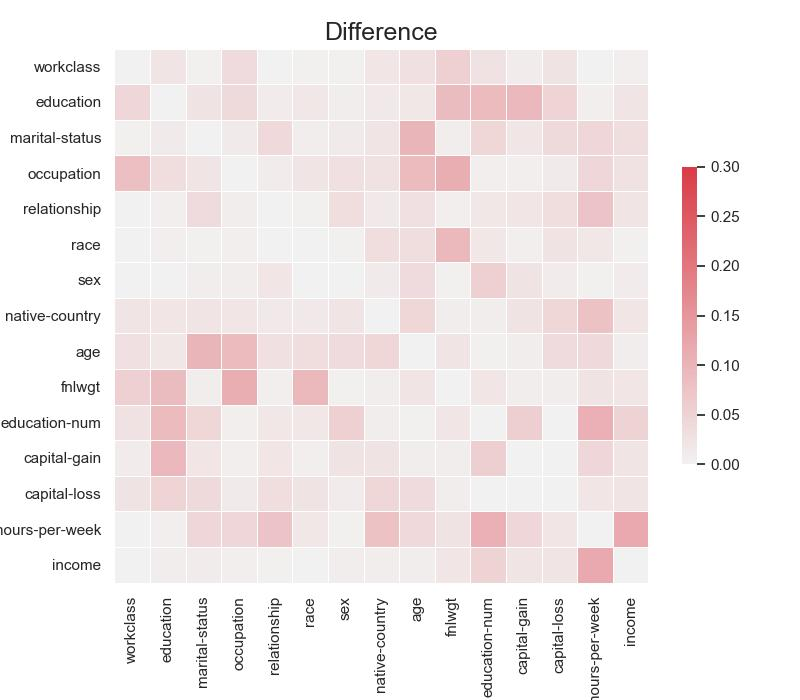
\includegraphics[width=\textwidth]{images/correlation_difference/ctabgan_simTune.jpg}
		\caption{CTABGAN$^s_q$}

	\end{subfigure}
    \begin{subfigure}{0.3\textwidth}
        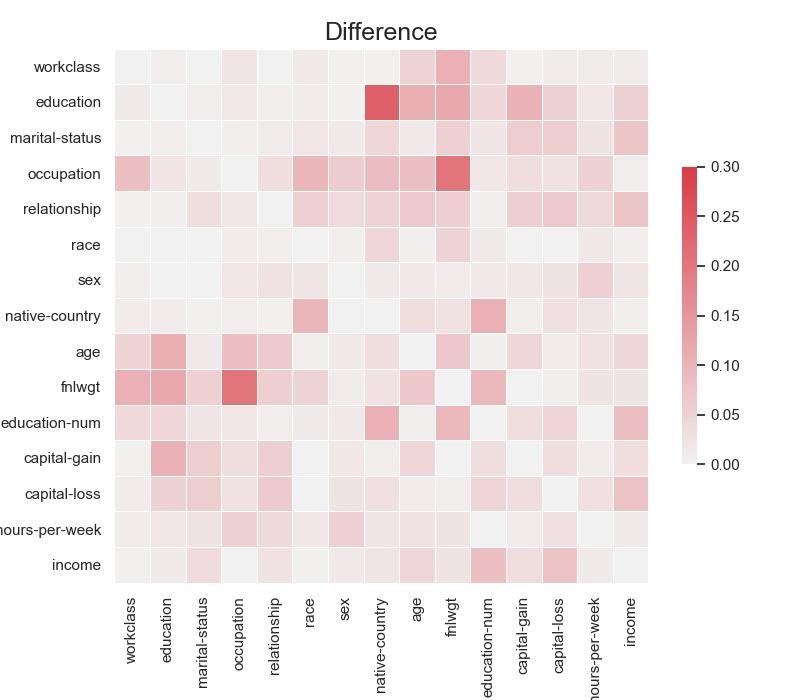
\includegraphics[width=\textwidth]{images/correlation_difference/tvae_simTune.jpg}
        \caption{TVAE$^s$}

    \end{subfigure}
	\begin{subfigure}{0.3\textwidth}
		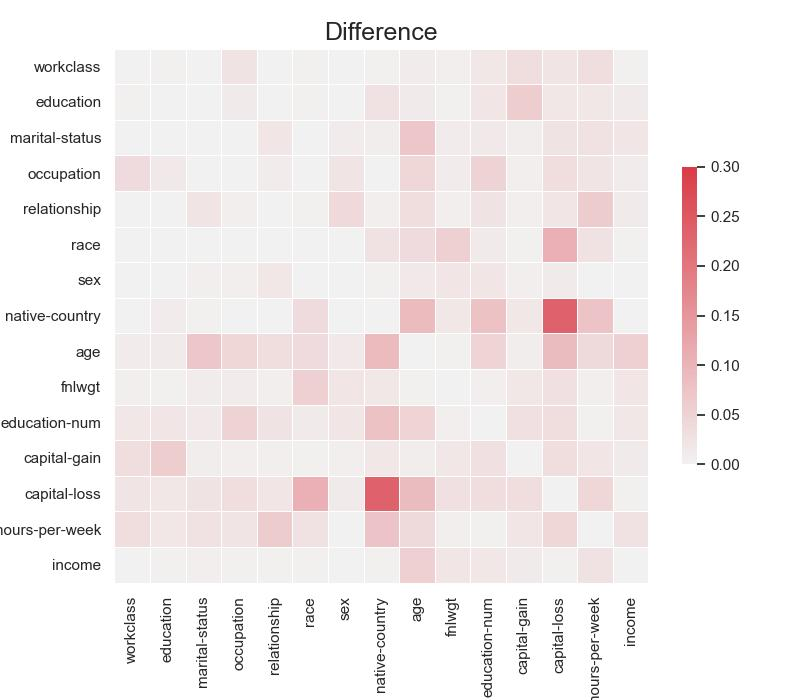
\includegraphics[width=\textwidth]{images/correlation_difference/tab-ddpm-bgm-simTune.jpg}
		\caption{TabDDPM-BGM$^{s}_q$}

	\end{subfigure}
    \begin{subfigure}{0.3\textwidth}
        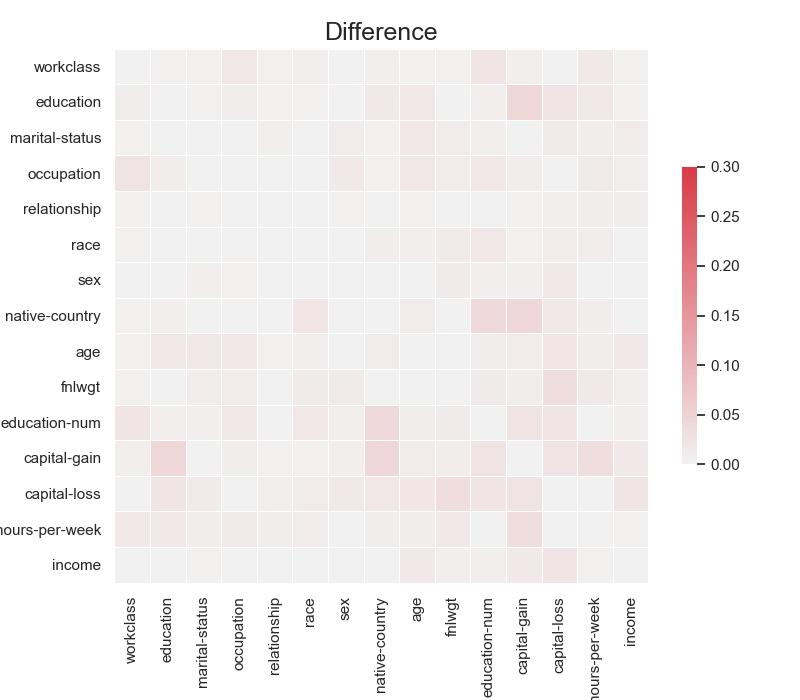
\includegraphics[width=\textwidth]{images/correlation_difference/tab-ddpm-bgm-simTune-minmax.jpg}
        \caption{TabDDPM-BGM$^{s}_m$}

    \end{subfigure}
	\begin{subfigure}{0.3\textwidth}
		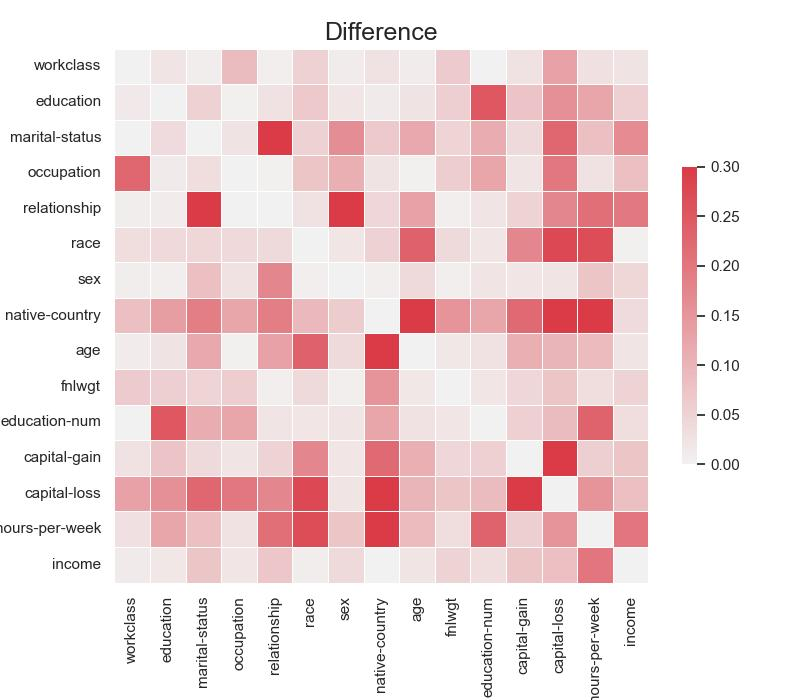
\includegraphics[width=\textwidth]{images/correlation_difference/tab-ddpm-ft-simTune.jpg}
		\caption{TabDDPM-FT$^{s}_q$}

    \end{subfigure}
    \caption{Correlation difference matrix for different model versions}

\end{figure}

\subsection[]{Principle Component Analysis}
\label{A:pca}

\begin{figure}[h]
	\centering
	\begin{subfigure}{0.3\textwidth}
		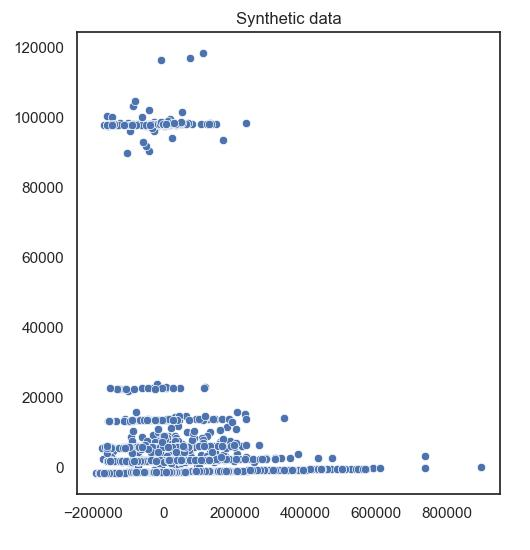
\includegraphics[width=\textwidth]{images/pca/ctabgan_simTune.jpg}
		\caption{CTABGAN$^s$}
	\end{subfigure}
    \begin{subfigure}{0.3\textwidth}
        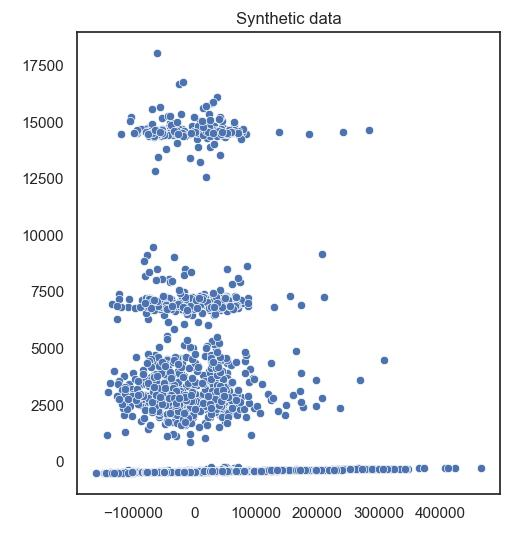
\includegraphics[width=\textwidth]{images/pca/tvae_simTune.jpg}
        \caption{TVAE$^s$}
    \end{subfigure}
	\begin{subfigure}{0.3\textwidth}
		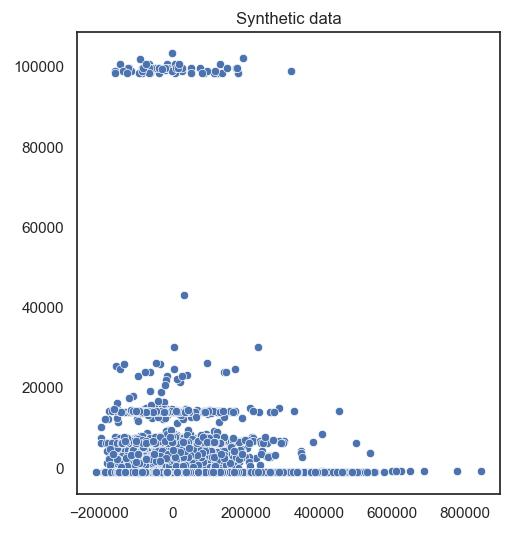
\includegraphics[width=\textwidth]{images/pca/tab-ddpm-bgm-simTune.jpg}
		\caption{TabDDPM-BGM$^{s}_q$}
	\end{subfigure}
	\begin{subfigure}{0.3\textwidth}
		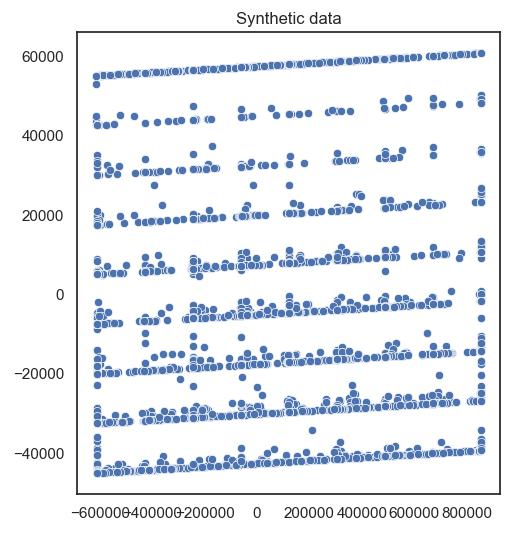
\includegraphics[width=\textwidth]{images/pca/tab-ddpm-ft-simTune.jpg}
		\caption{TabDDPM-FT$^{s}_q$}
    \end{subfigure}
	\begin{subfigure}{0.3\textwidth}
		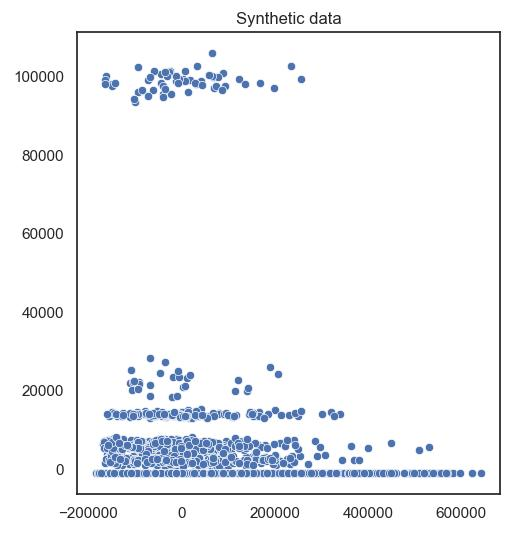
\includegraphics[width=\textwidth]{images/pca/tab-ddpm-bgm-simTune-minmax.jpg}
		\caption{TabDDPM-BGM$^{s}_m$}
		\label{fig_a:pca_TabDDPMBM}
    \end{subfigure}
    \caption{Principle Component Analysisfor different model versions}
    \label{fig_a:pca_diff}
\end{figure}

\subsection[]{Distribution Plots}
\label{A:distributions}
%----------
\newpage
\begin{landscape}
	\begin{figure}[h]
		\centering
		\hfill
		\begin{subfigure}{0.3\linewidth}
			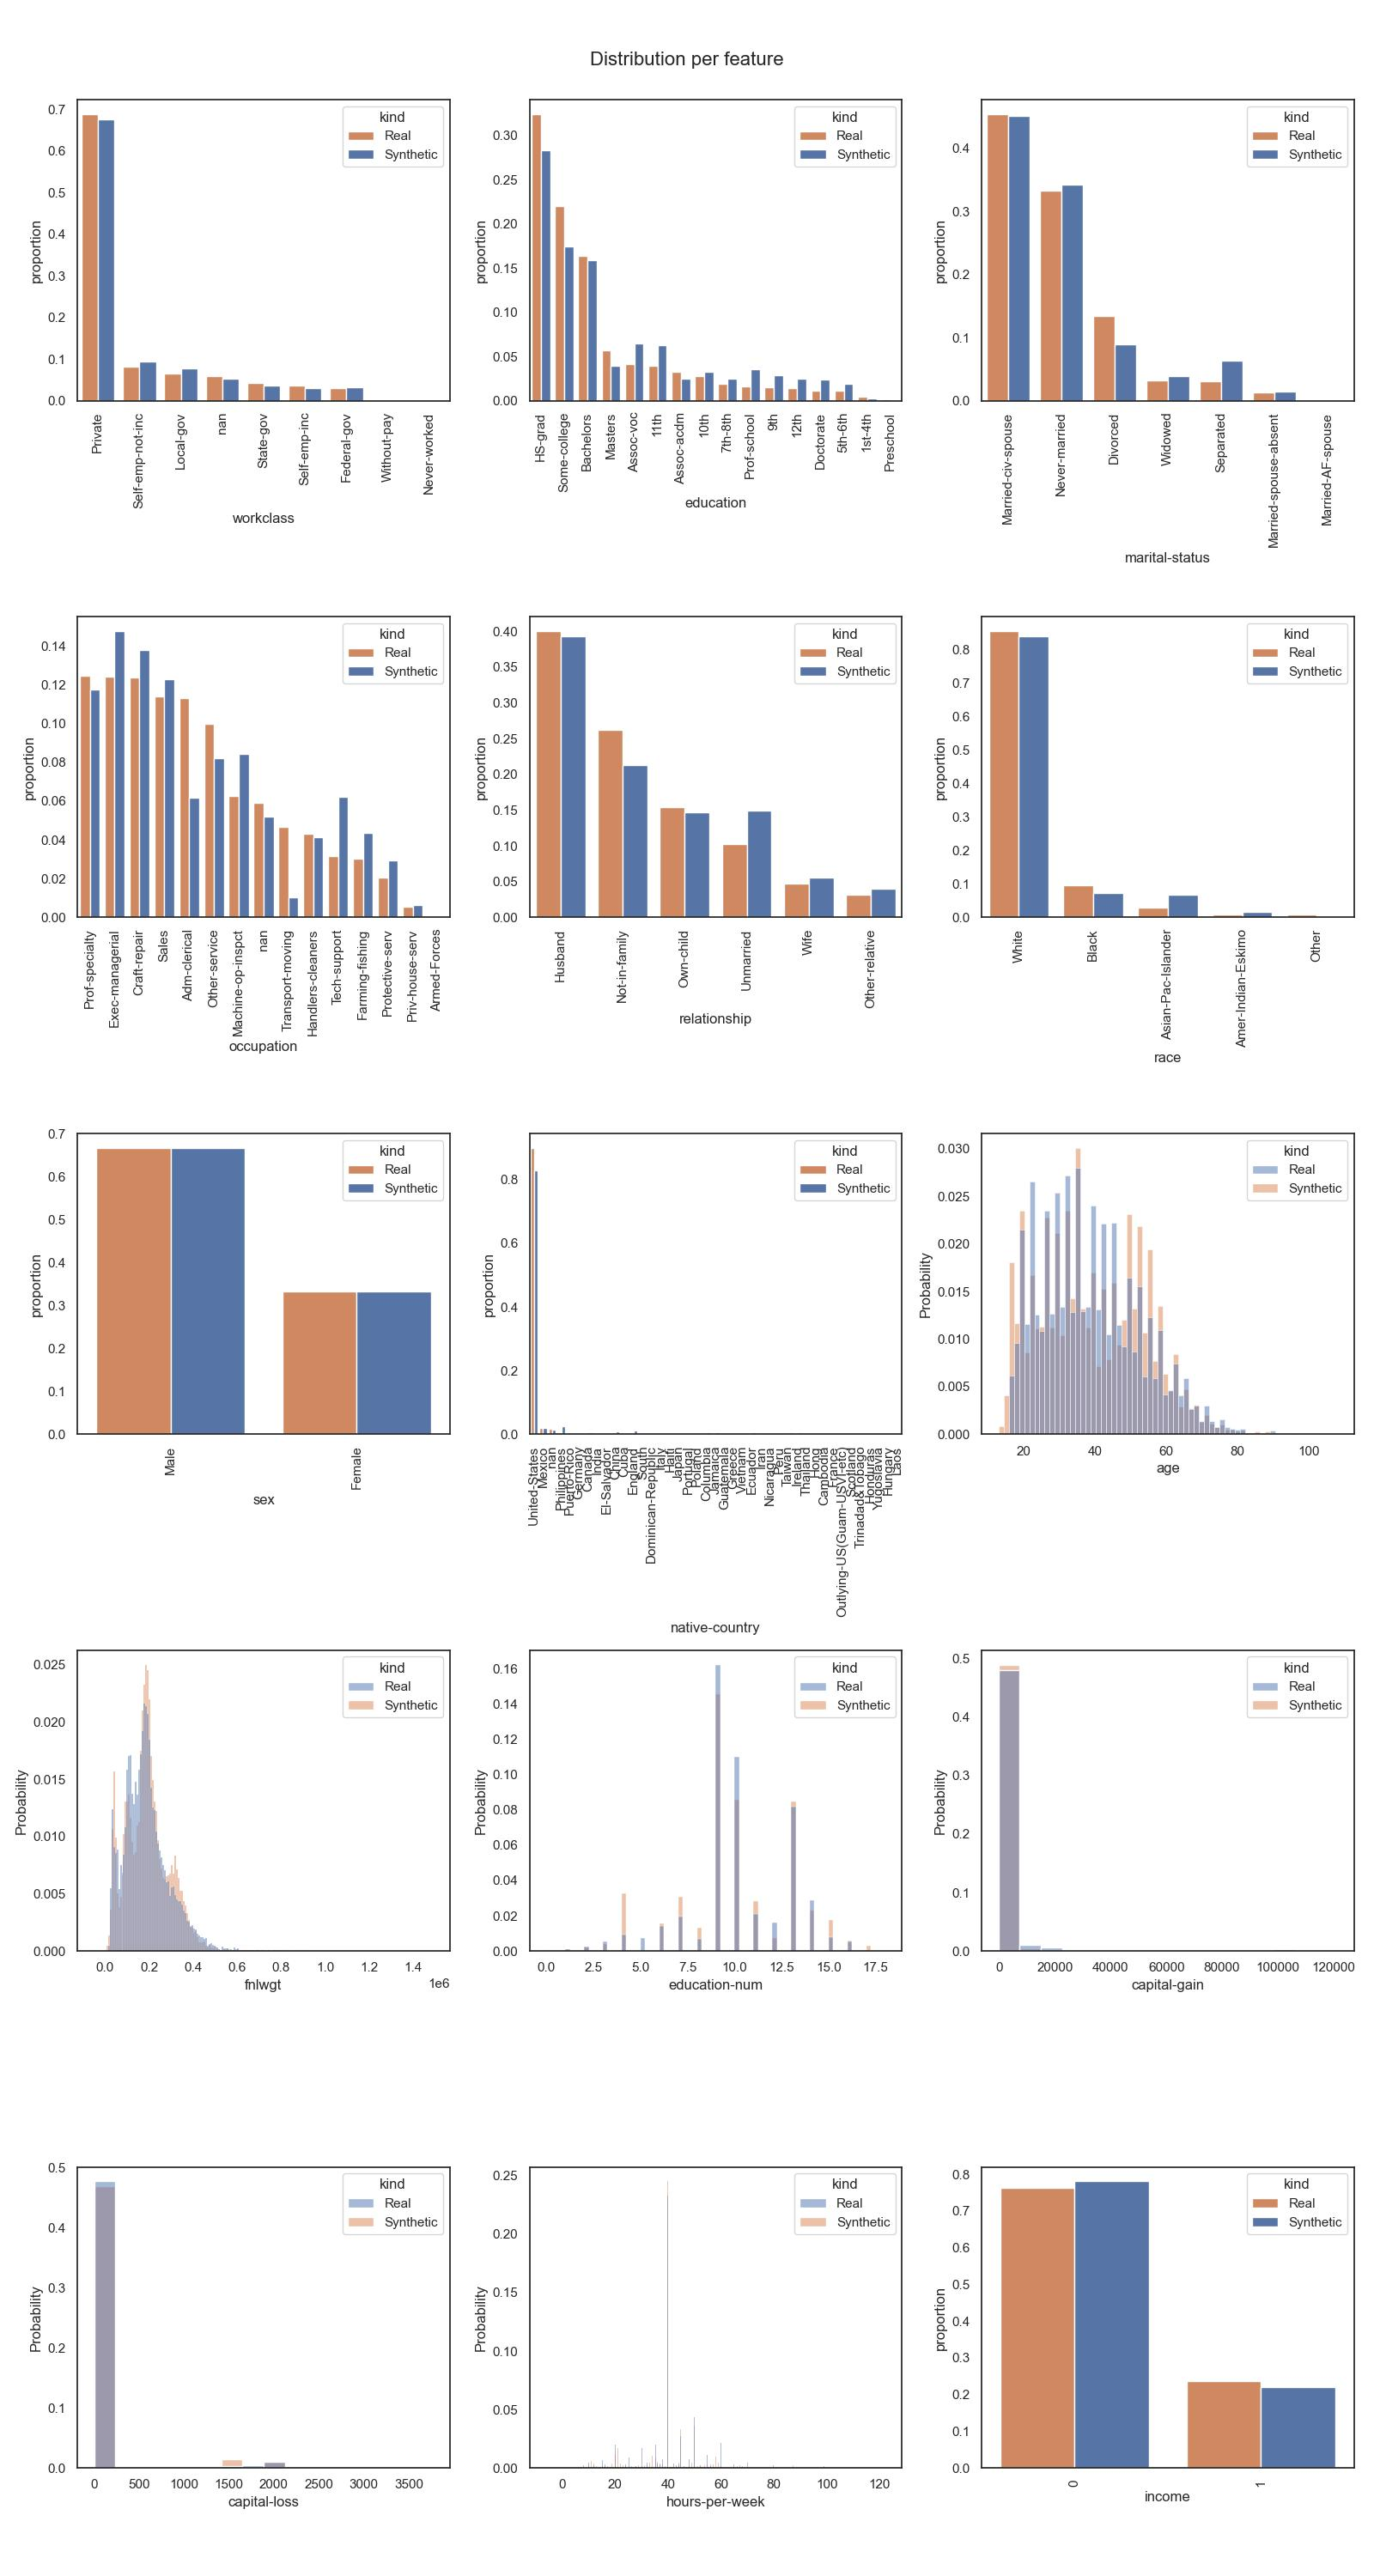
\includegraphics[height=\textheight,width=\linewidth,keepaspectratio]{images/distributions_full/ctabgan.jpg}
			\caption{CTABGAN$^{ml}$}
		\end{subfigure}
		\hfill
		\begin{subfigure}{0.3\linewidth}
			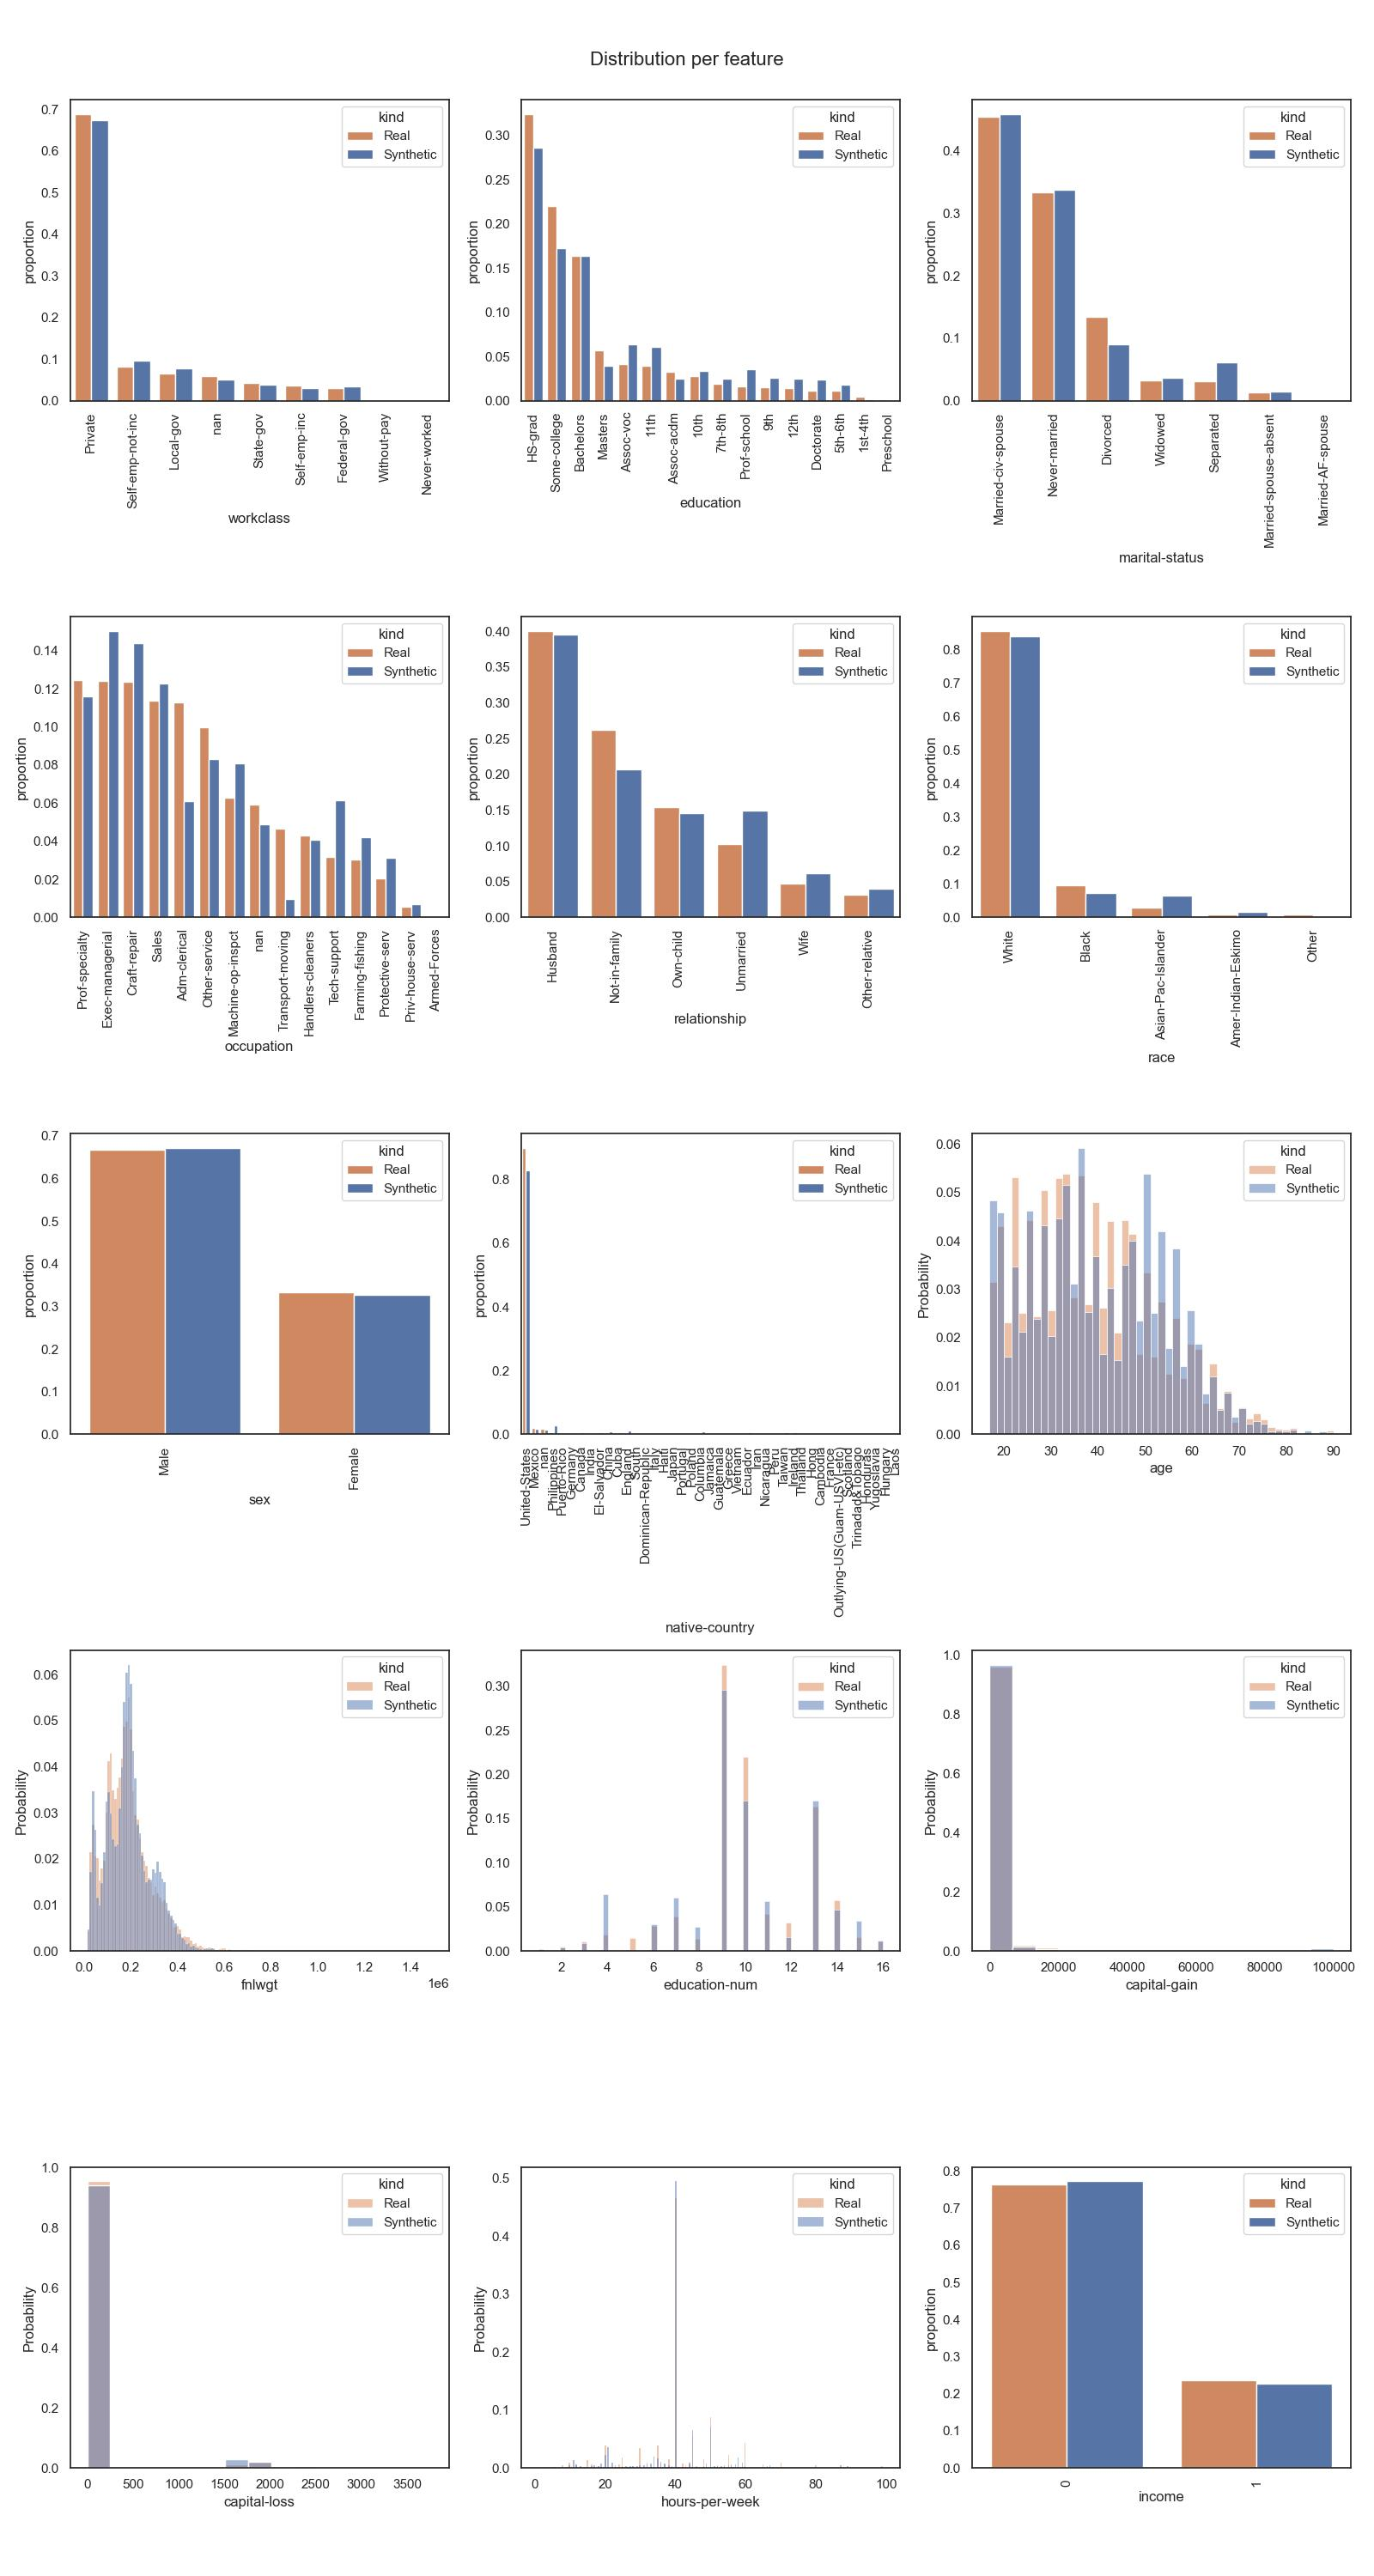
\includegraphics[height=\textheight,width=\linewidth,keepaspectratio]{images/distributions_full/ctabgan_simTune.jpg}
			\caption{CTABGAN$^s$}
		\end{subfigure}	
		\hfill
		\begin{subfigure}{0.3\linewidth}
			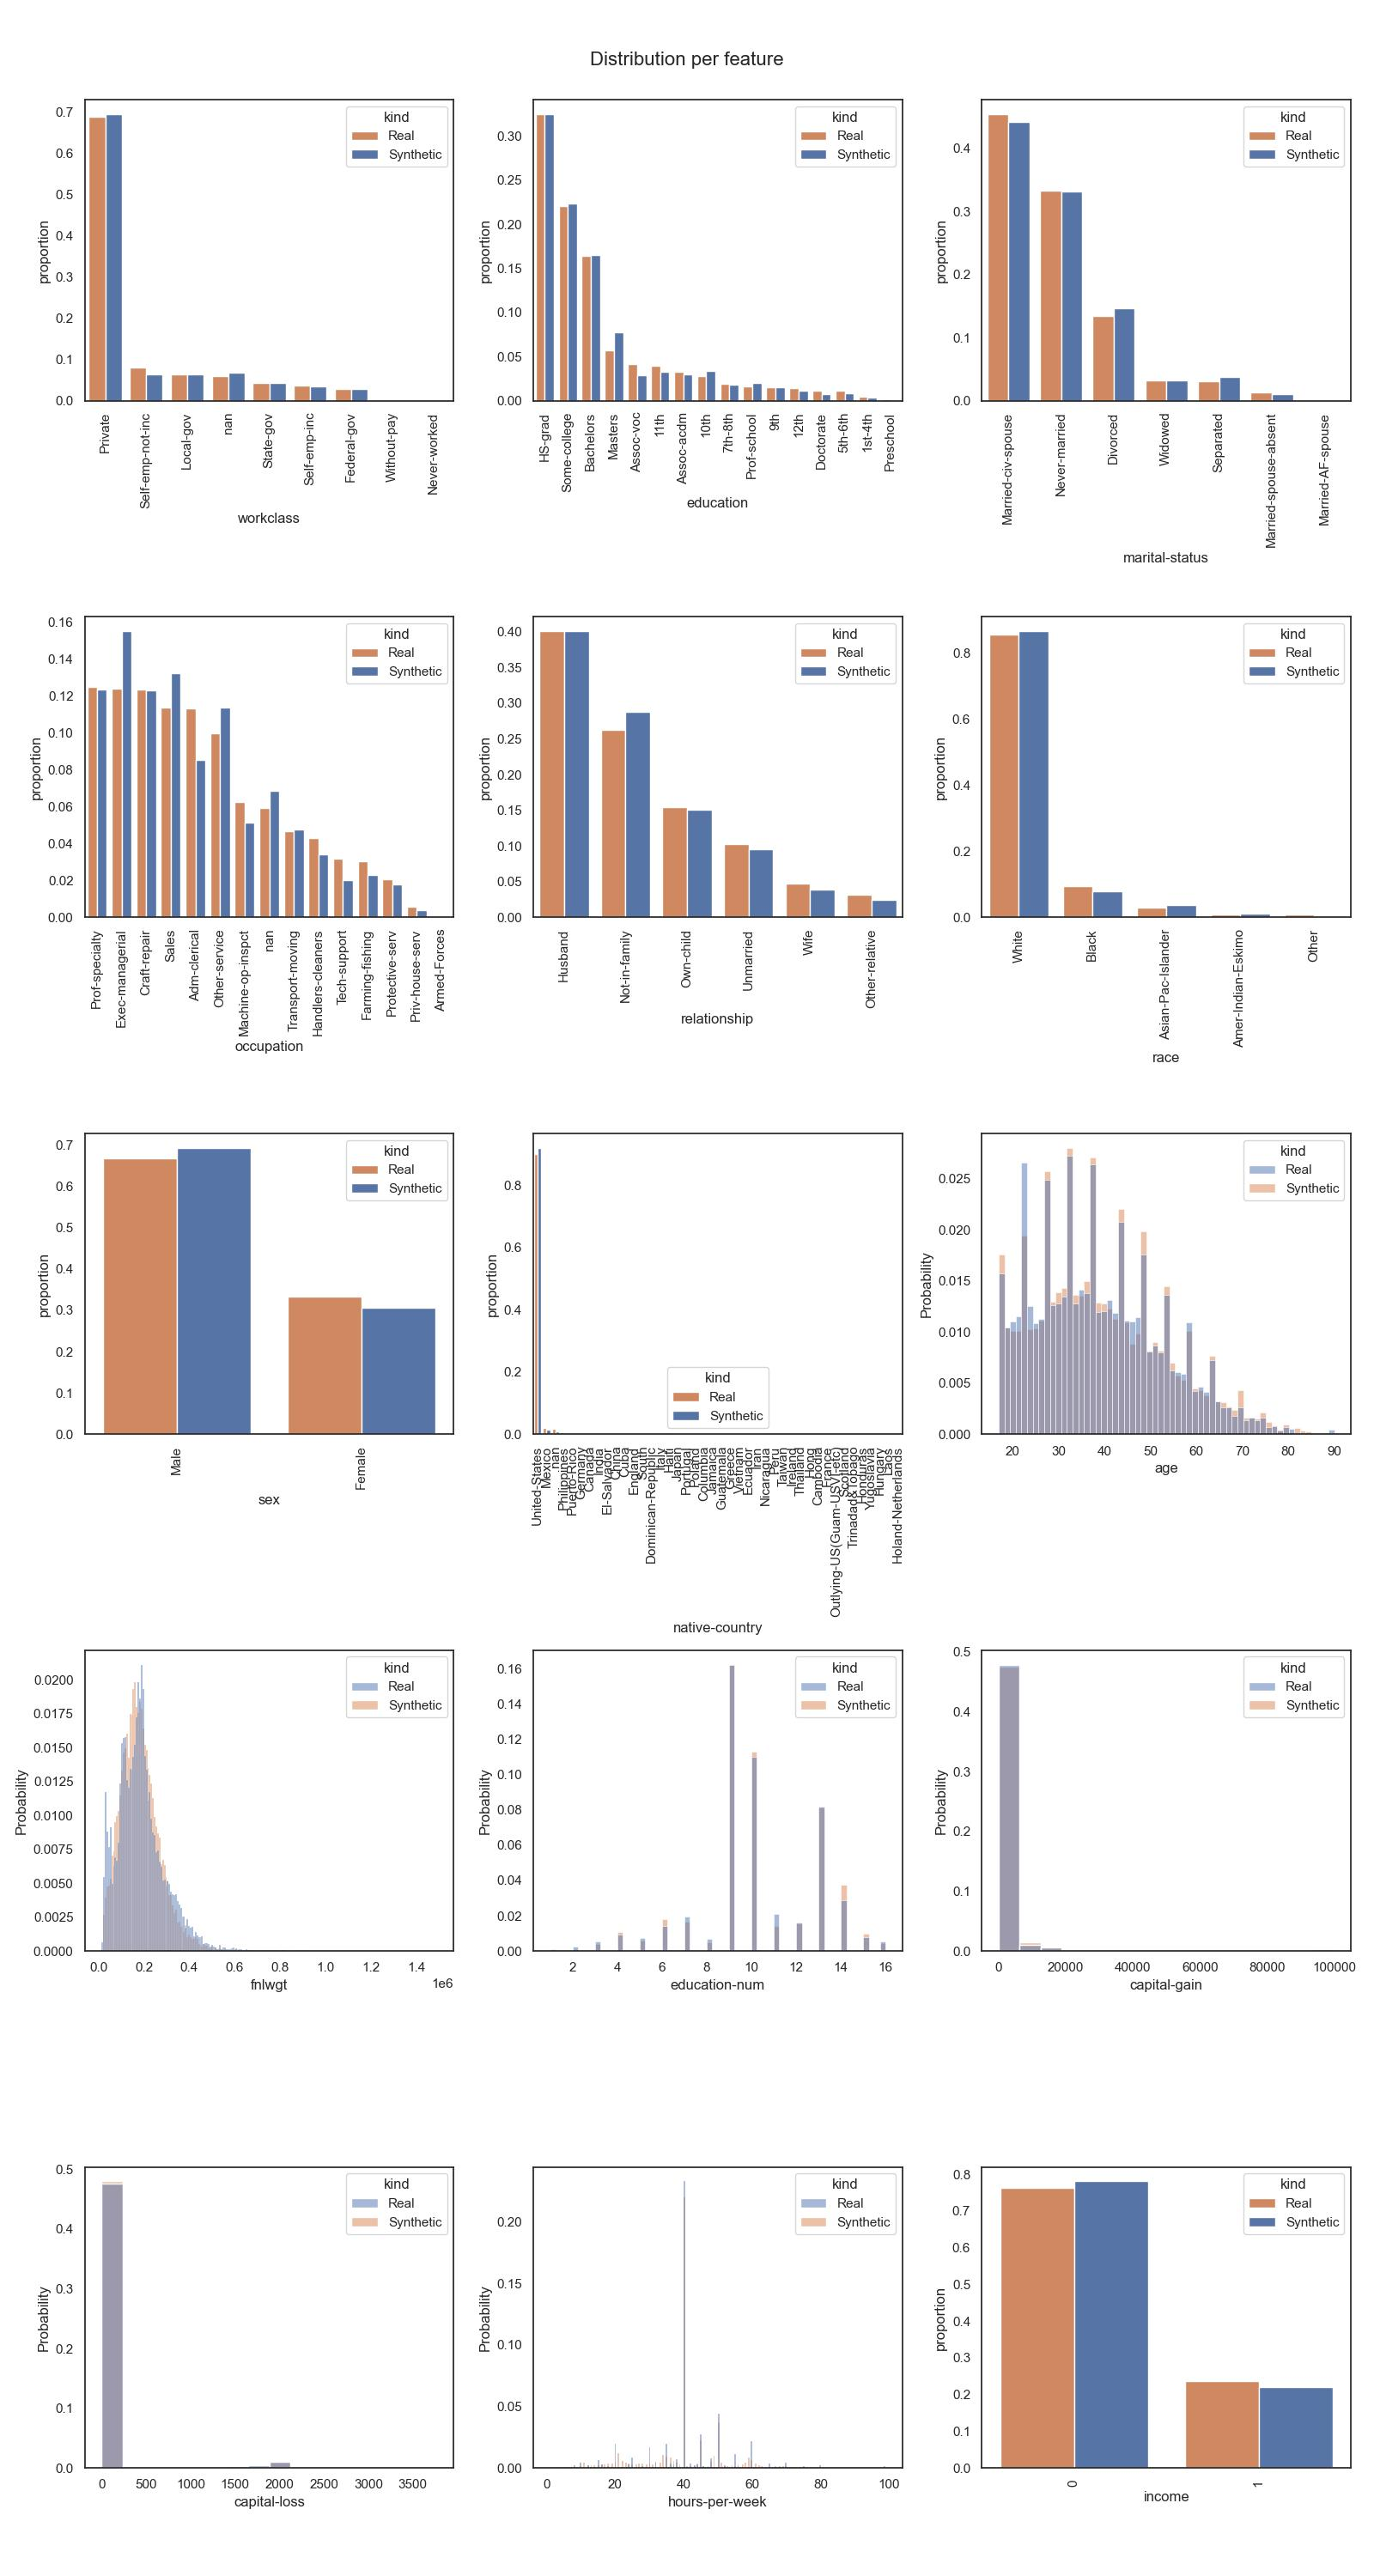
\includegraphics[height=\textheight,width=\linewidth,keepaspectratio]{images/distributions_full/ctabgan+.jpg}
			\caption{CTABGAN+$^{ml}$}
		\end{subfigure}
		\hfill
		\caption{Distribution plots for CTABGAN$^{ml}$, CTABGAN$^s$ and CTABGAN+$^{ml}$}
		\label{fig_a:dist_1}
	\end{figure}
\end{landscape}
%----------
\newpage
\begin{landscape}
	\begin{figure}[h]
		\centering
		\hfill
		\begin{subfigure}{0.3\linewidth}
			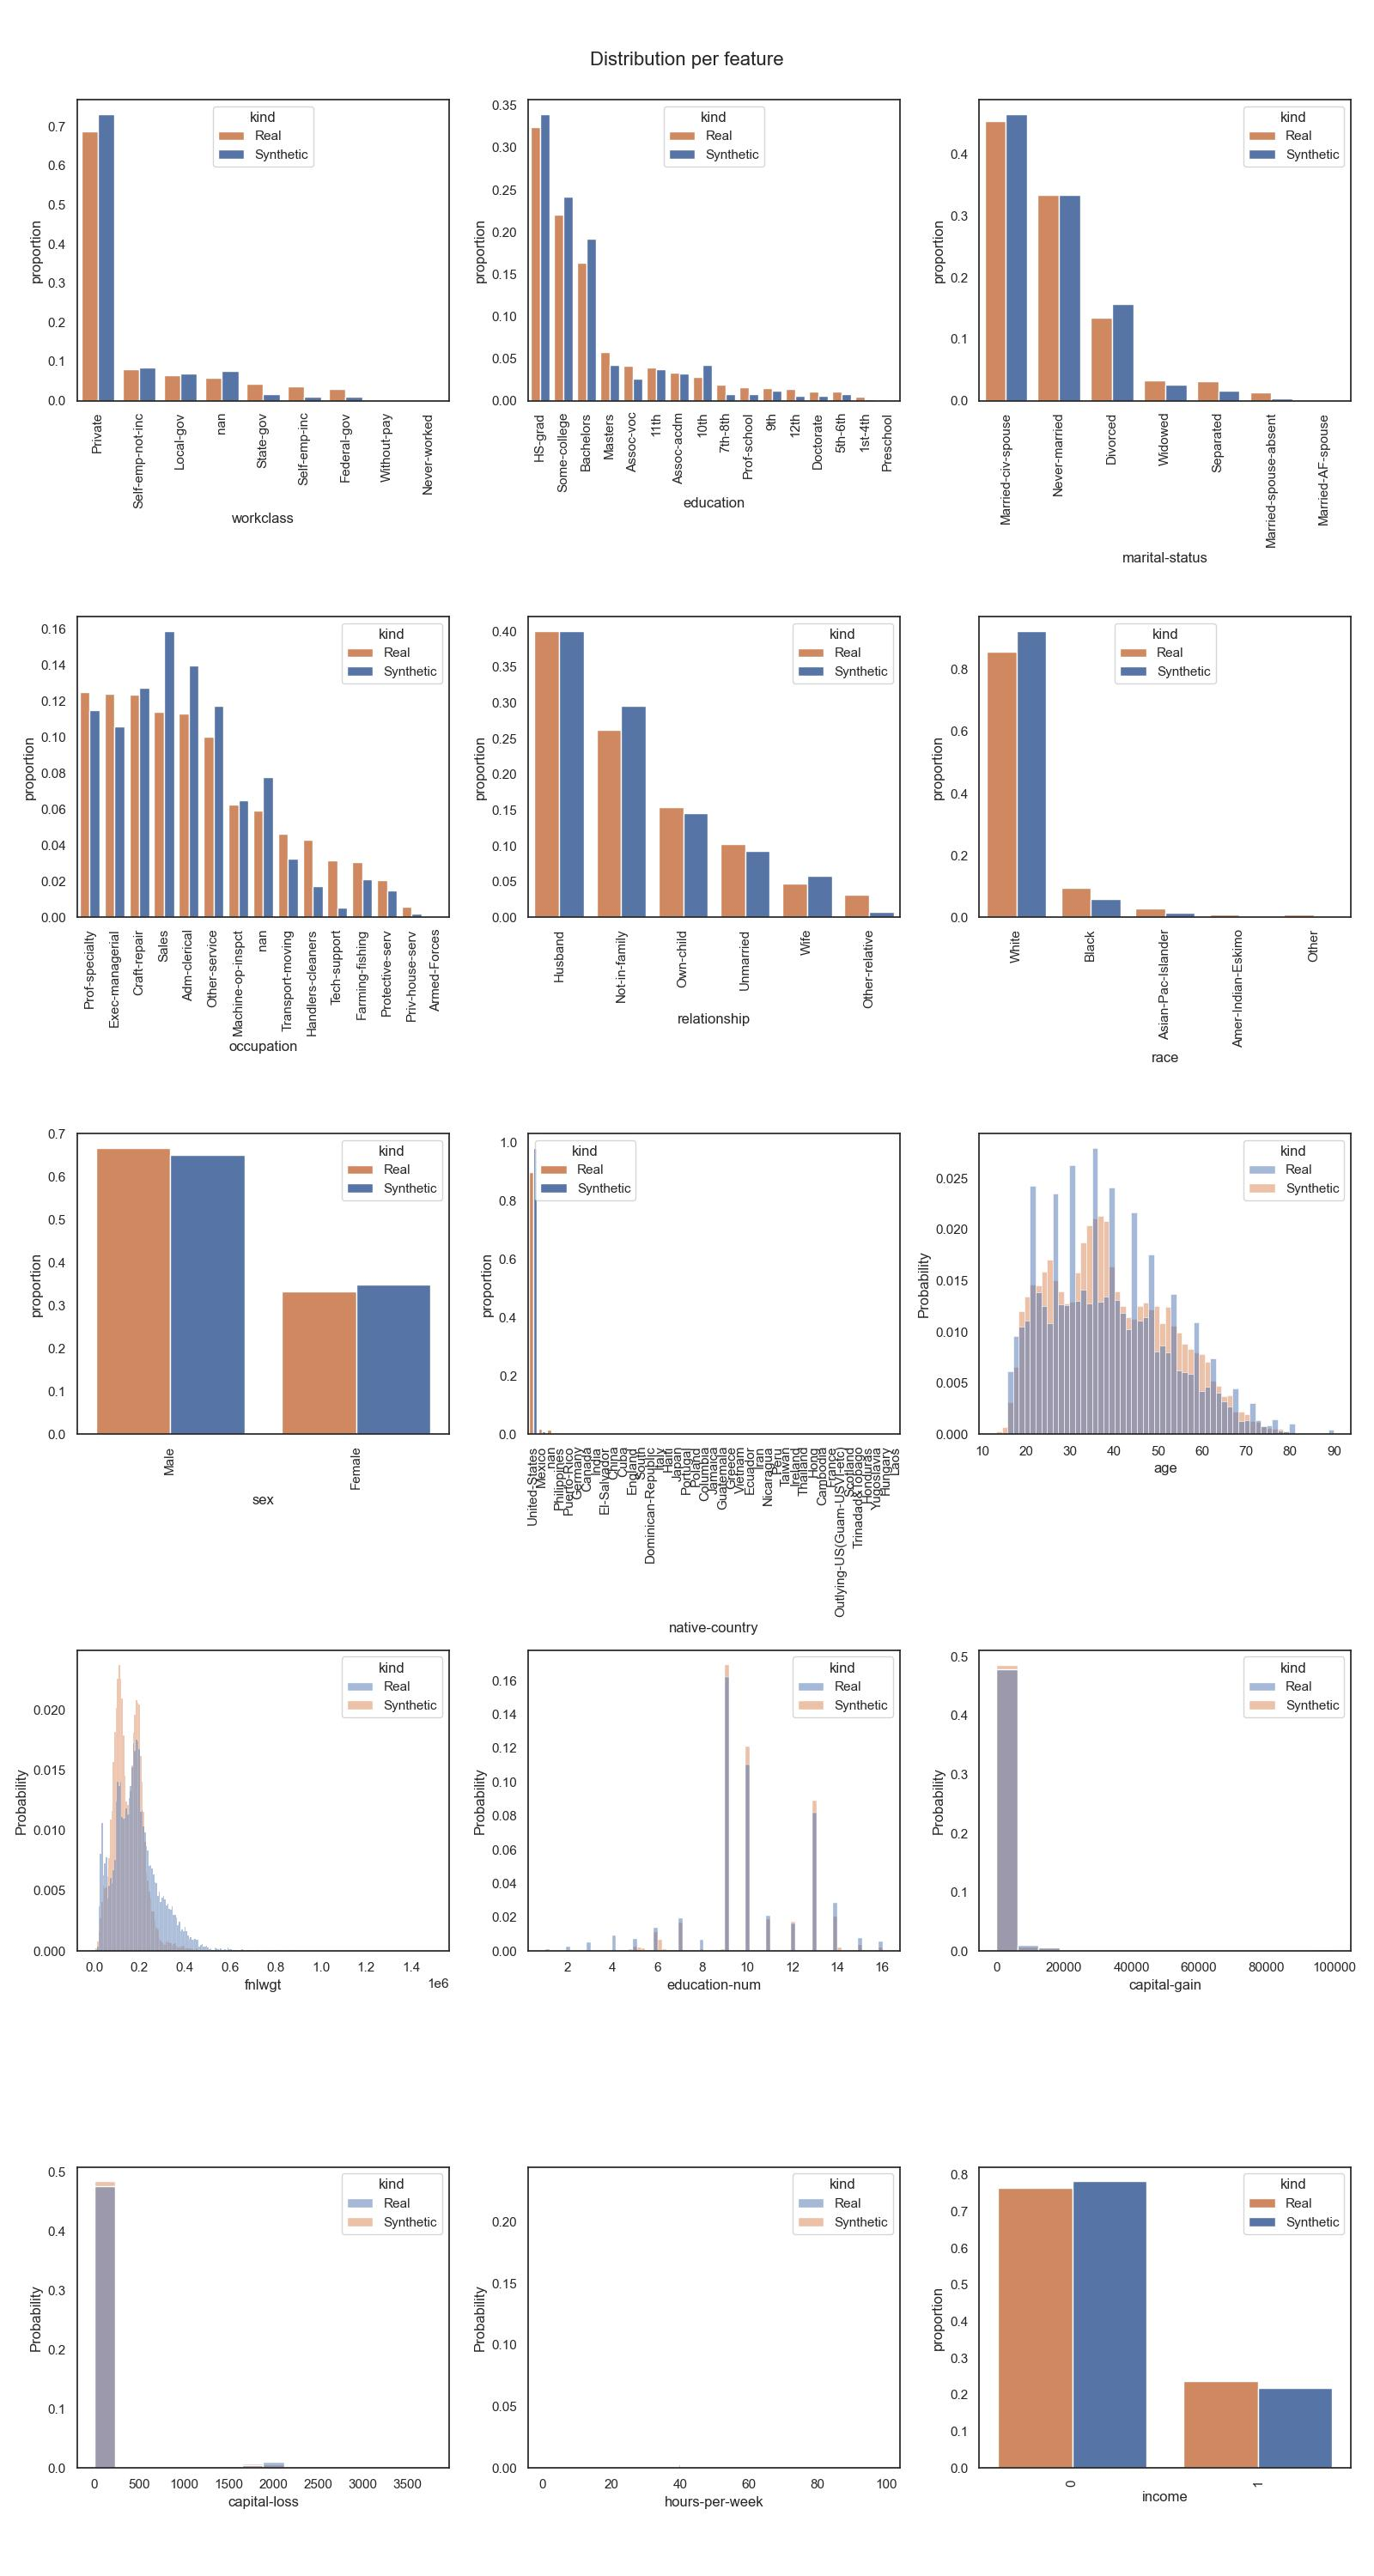
\includegraphics[height=\textheight,width=\linewidth,keepaspectratio]{images/distributions_full/tvae.jpg}
			\caption{TVAE$^{ml}$}
		\end{subfigure}		
		\hfill
		\begin{subfigure}{0.3\linewidth}
			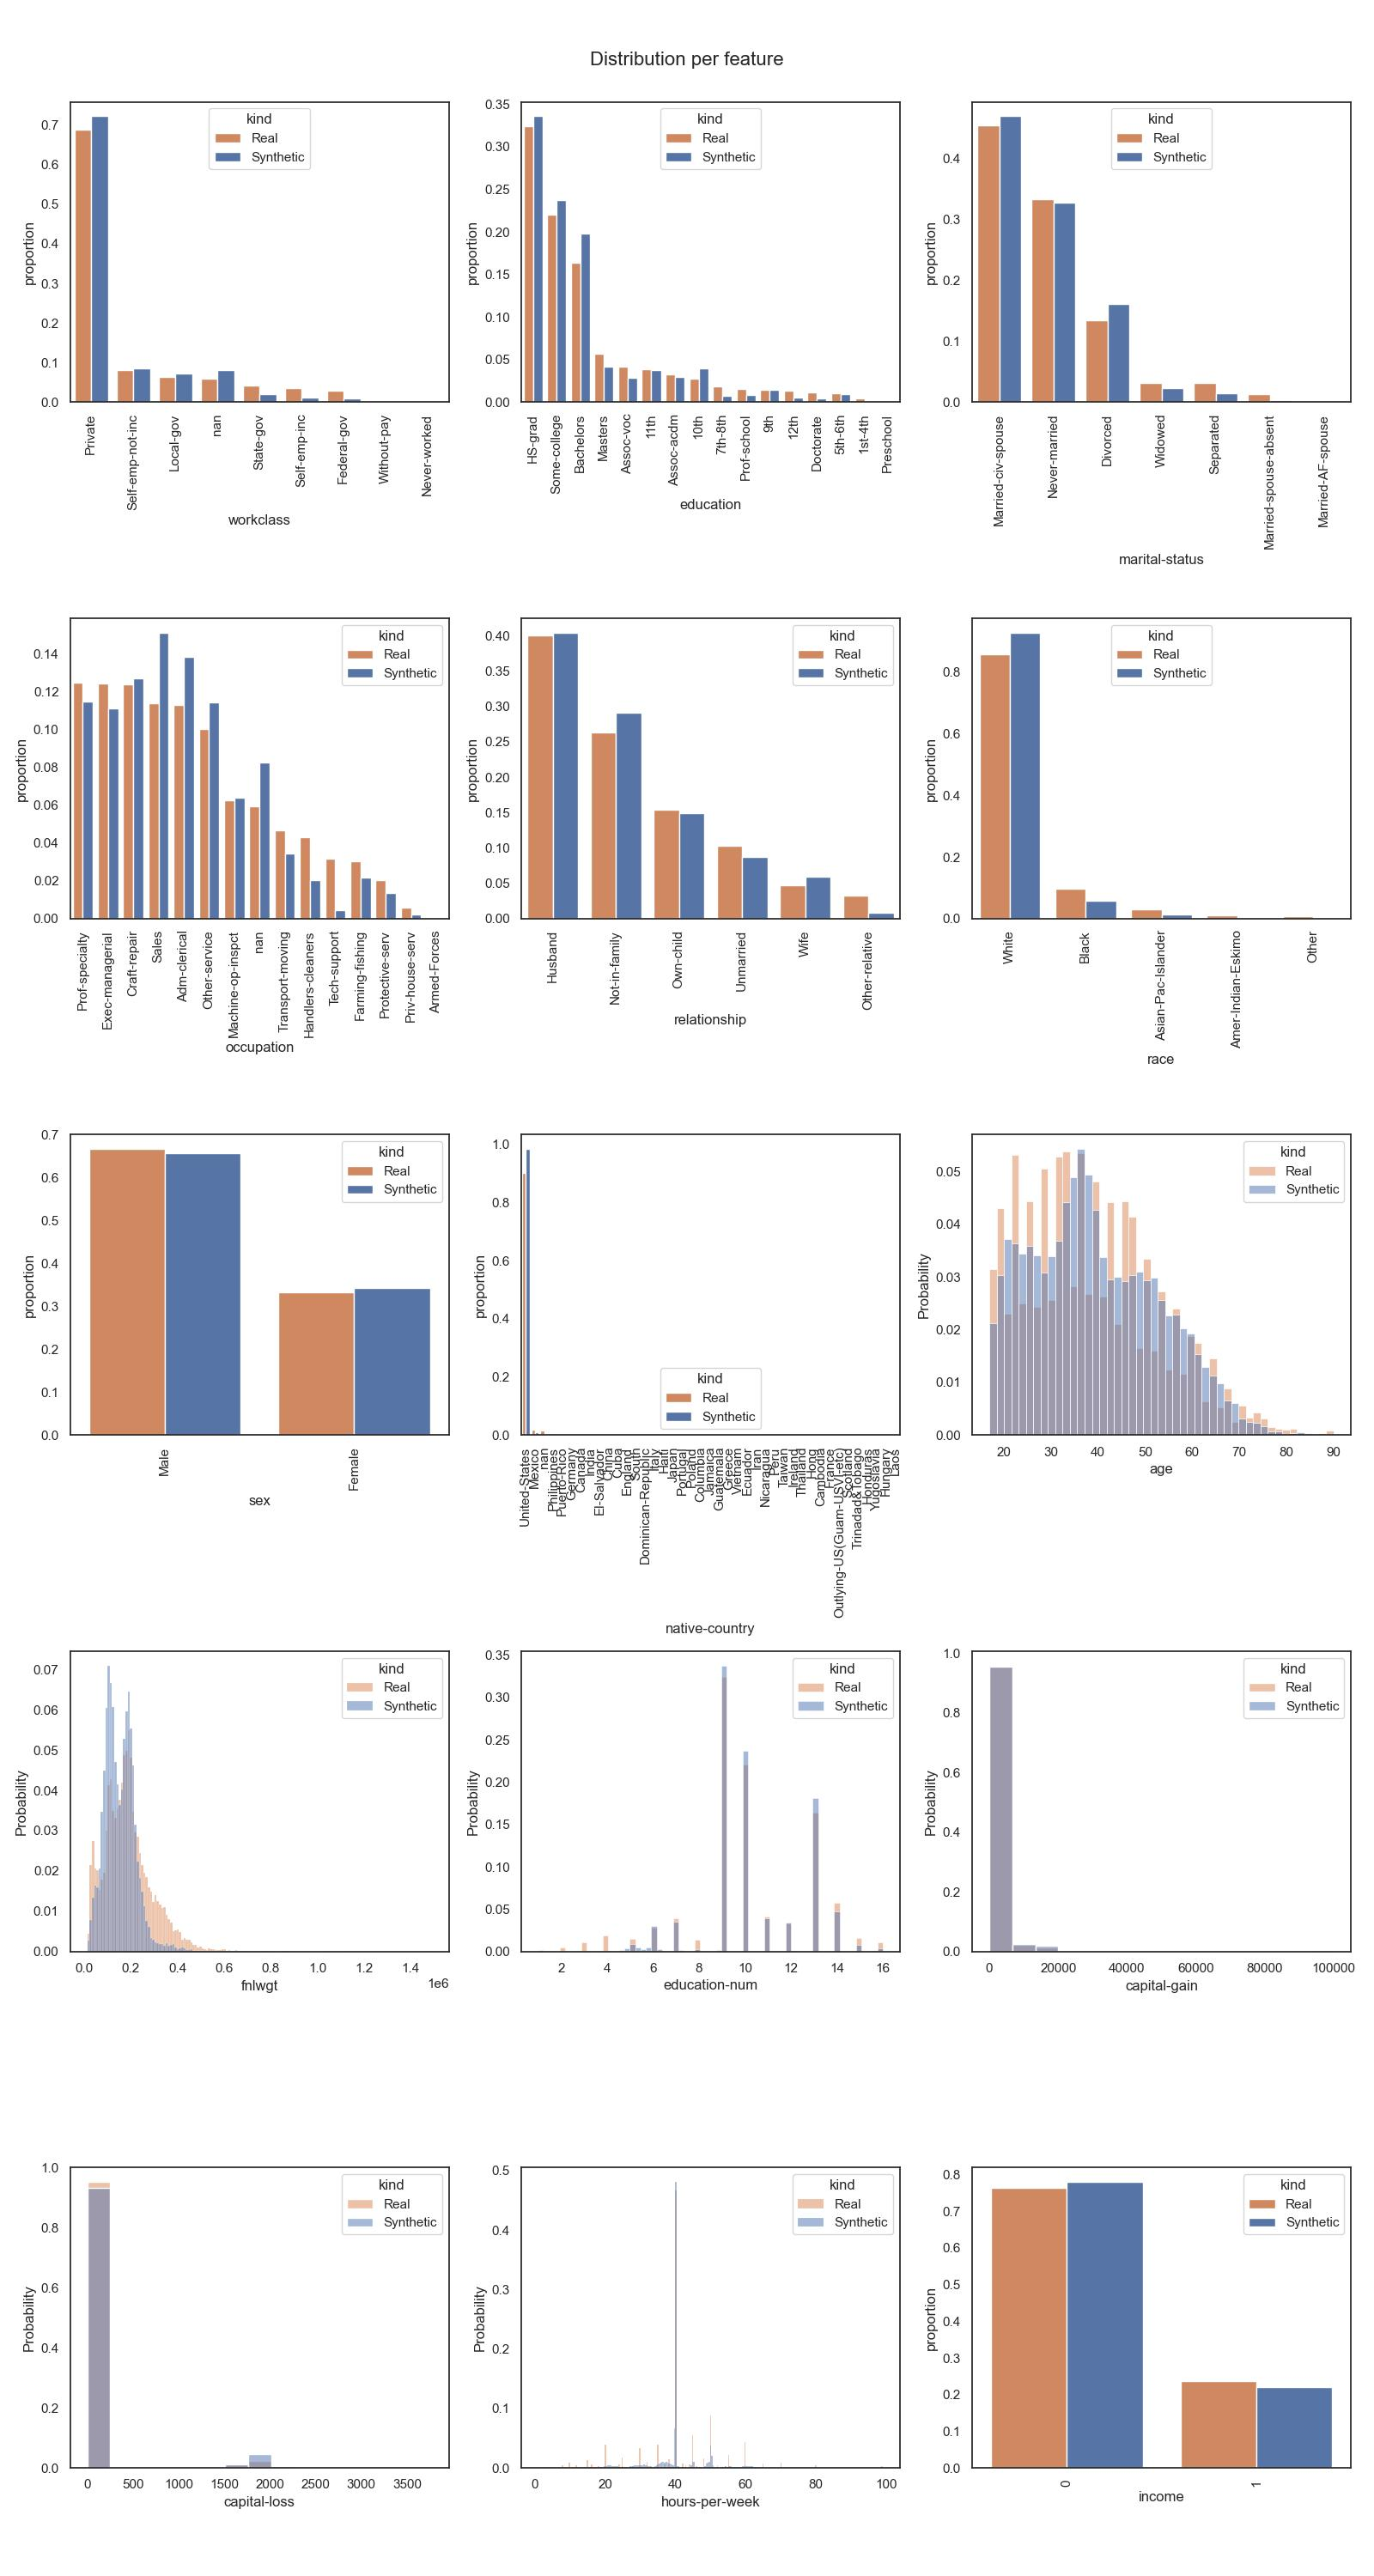
\includegraphics[height=\textheight,width=\linewidth,keepaspectratio]{images/distributions_full/tvae_simTune.jpg}
			\caption{TVAE$^s$}
		\end{subfigure}
		\hfill
		\begin{subfigure}{0.3\linewidth}
			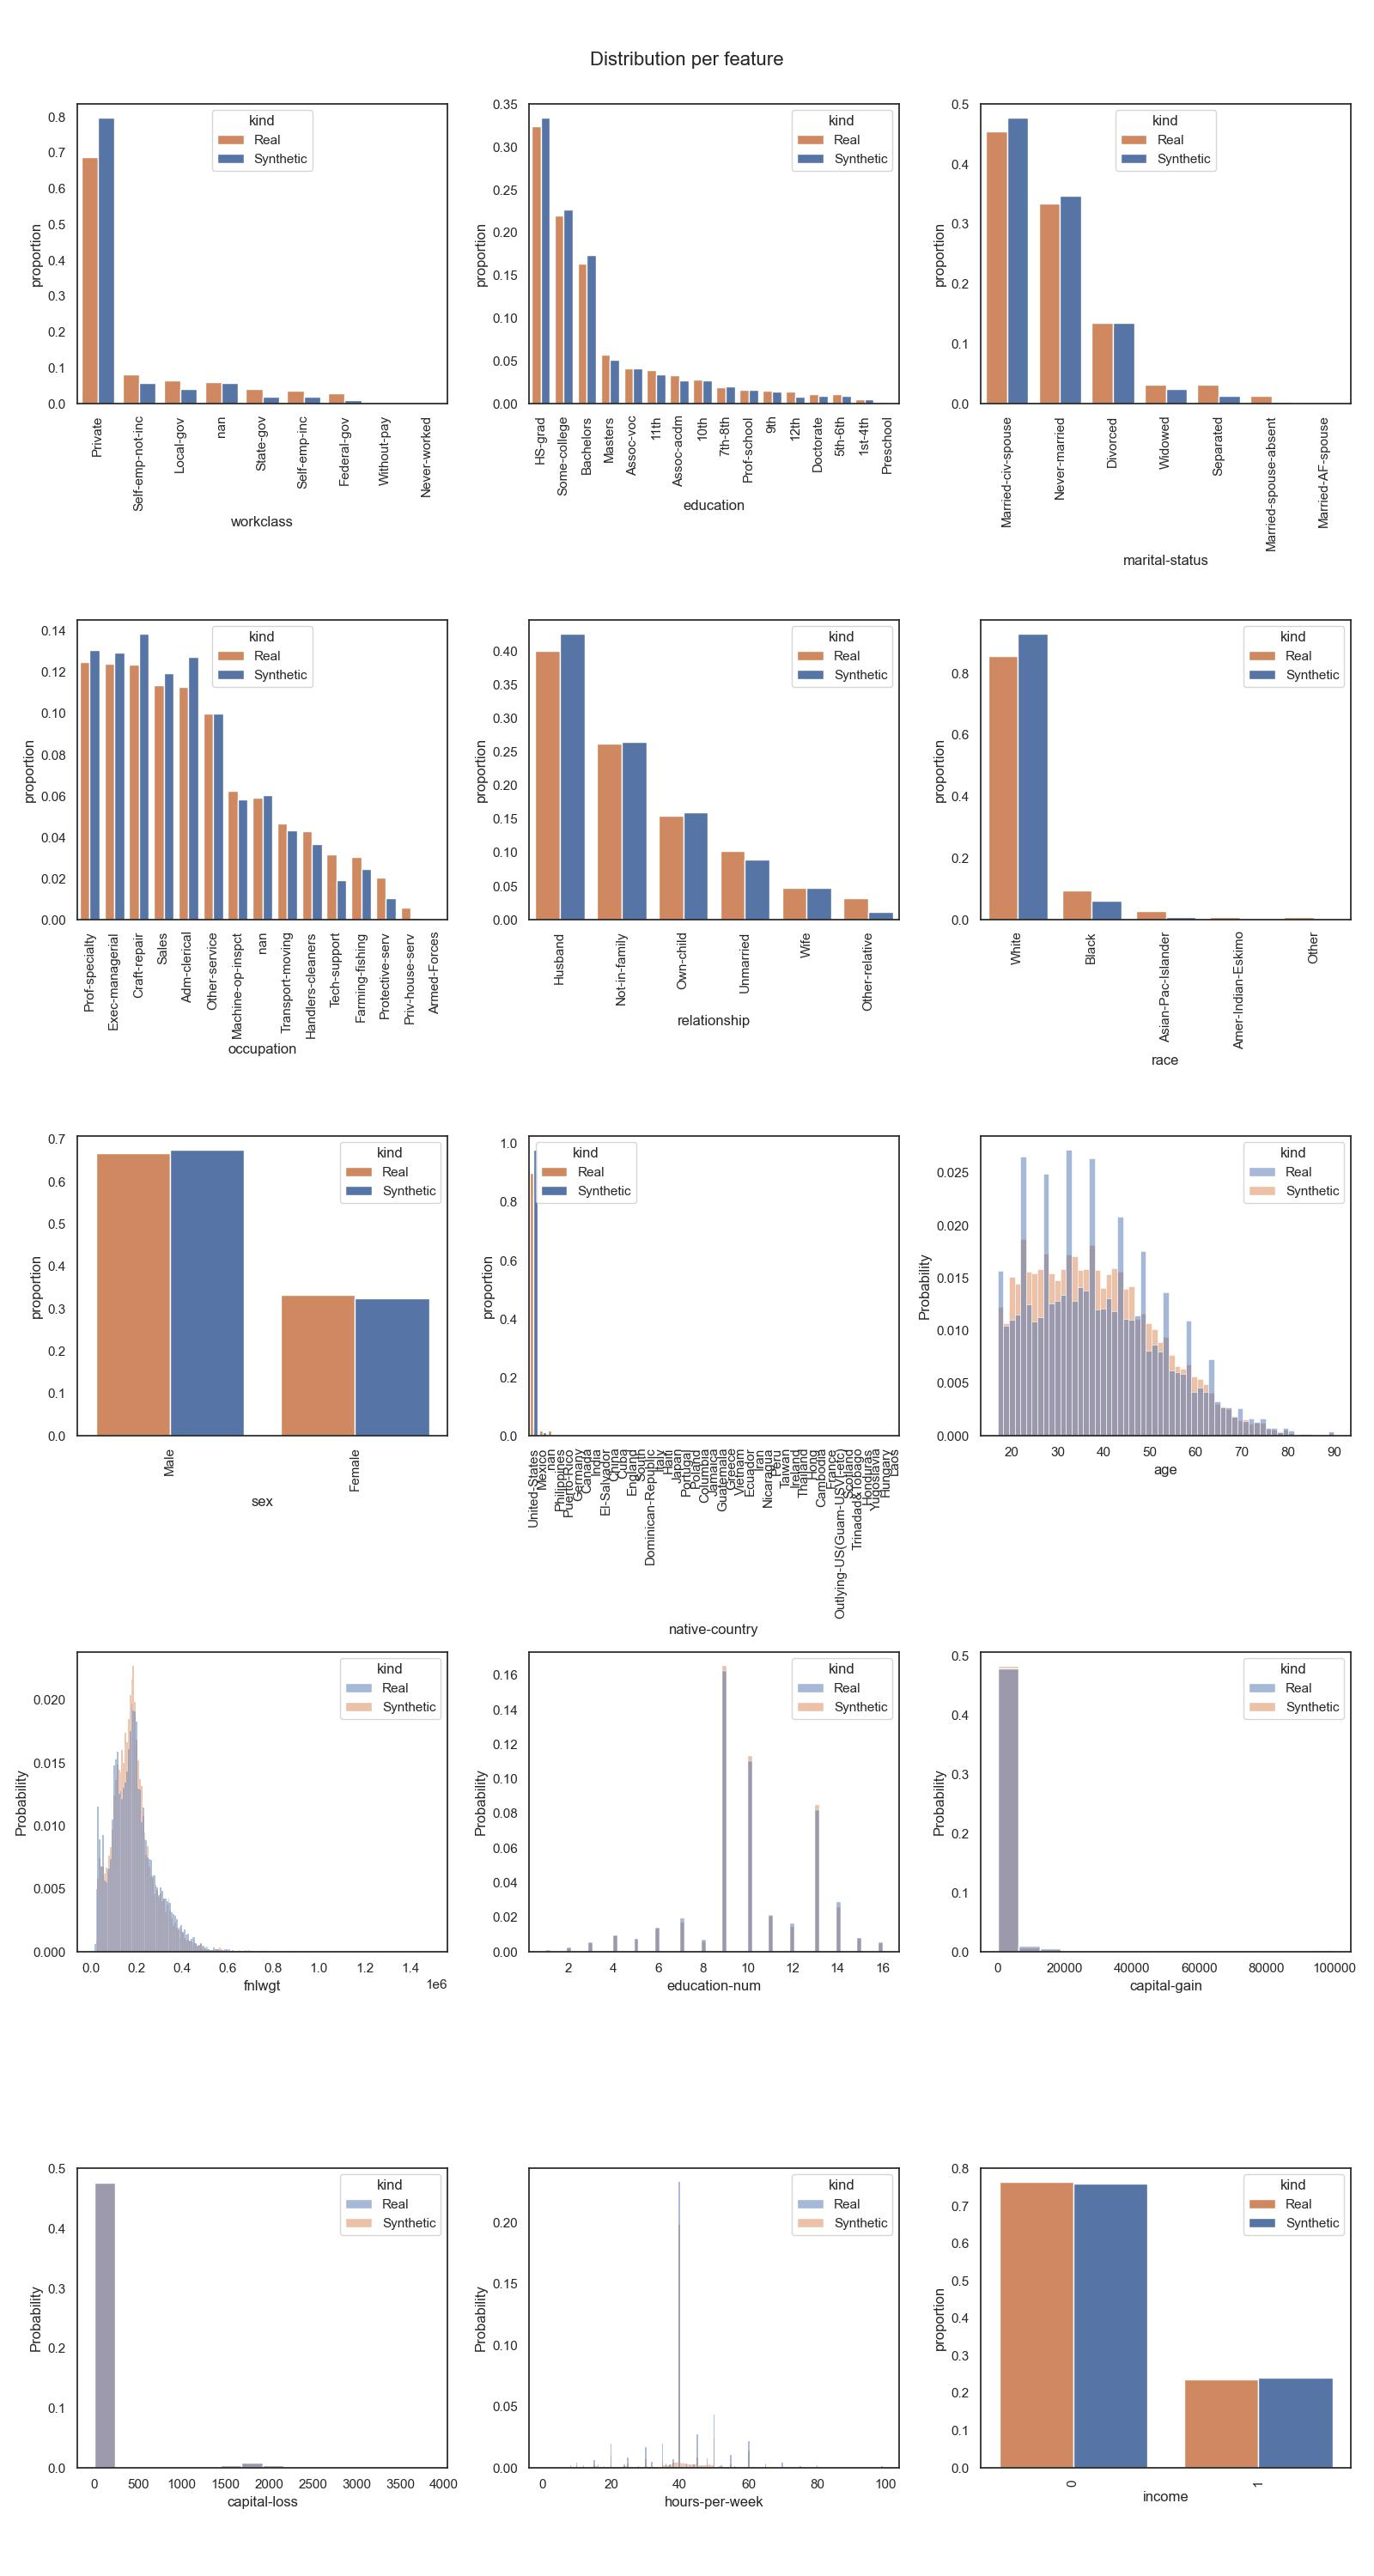
\includegraphics[height=\textheight,width=\linewidth,keepaspectratio]{images/distributions_full/smote.jpg}
			\caption{SMOTE}
		\end{subfigure}
		\caption{Distribution plots for TVAE$^{ml}$, TVAE$^s$ and SMOTE}
		\label{fig_a:dist_2}
	\end{figure}
\end{landscape}
%----------
\newpage
\begin{landscape}
	\begin{figure}[h]
		\centering
		\hfill
		\begin{subfigure}{0.3\linewidth}
			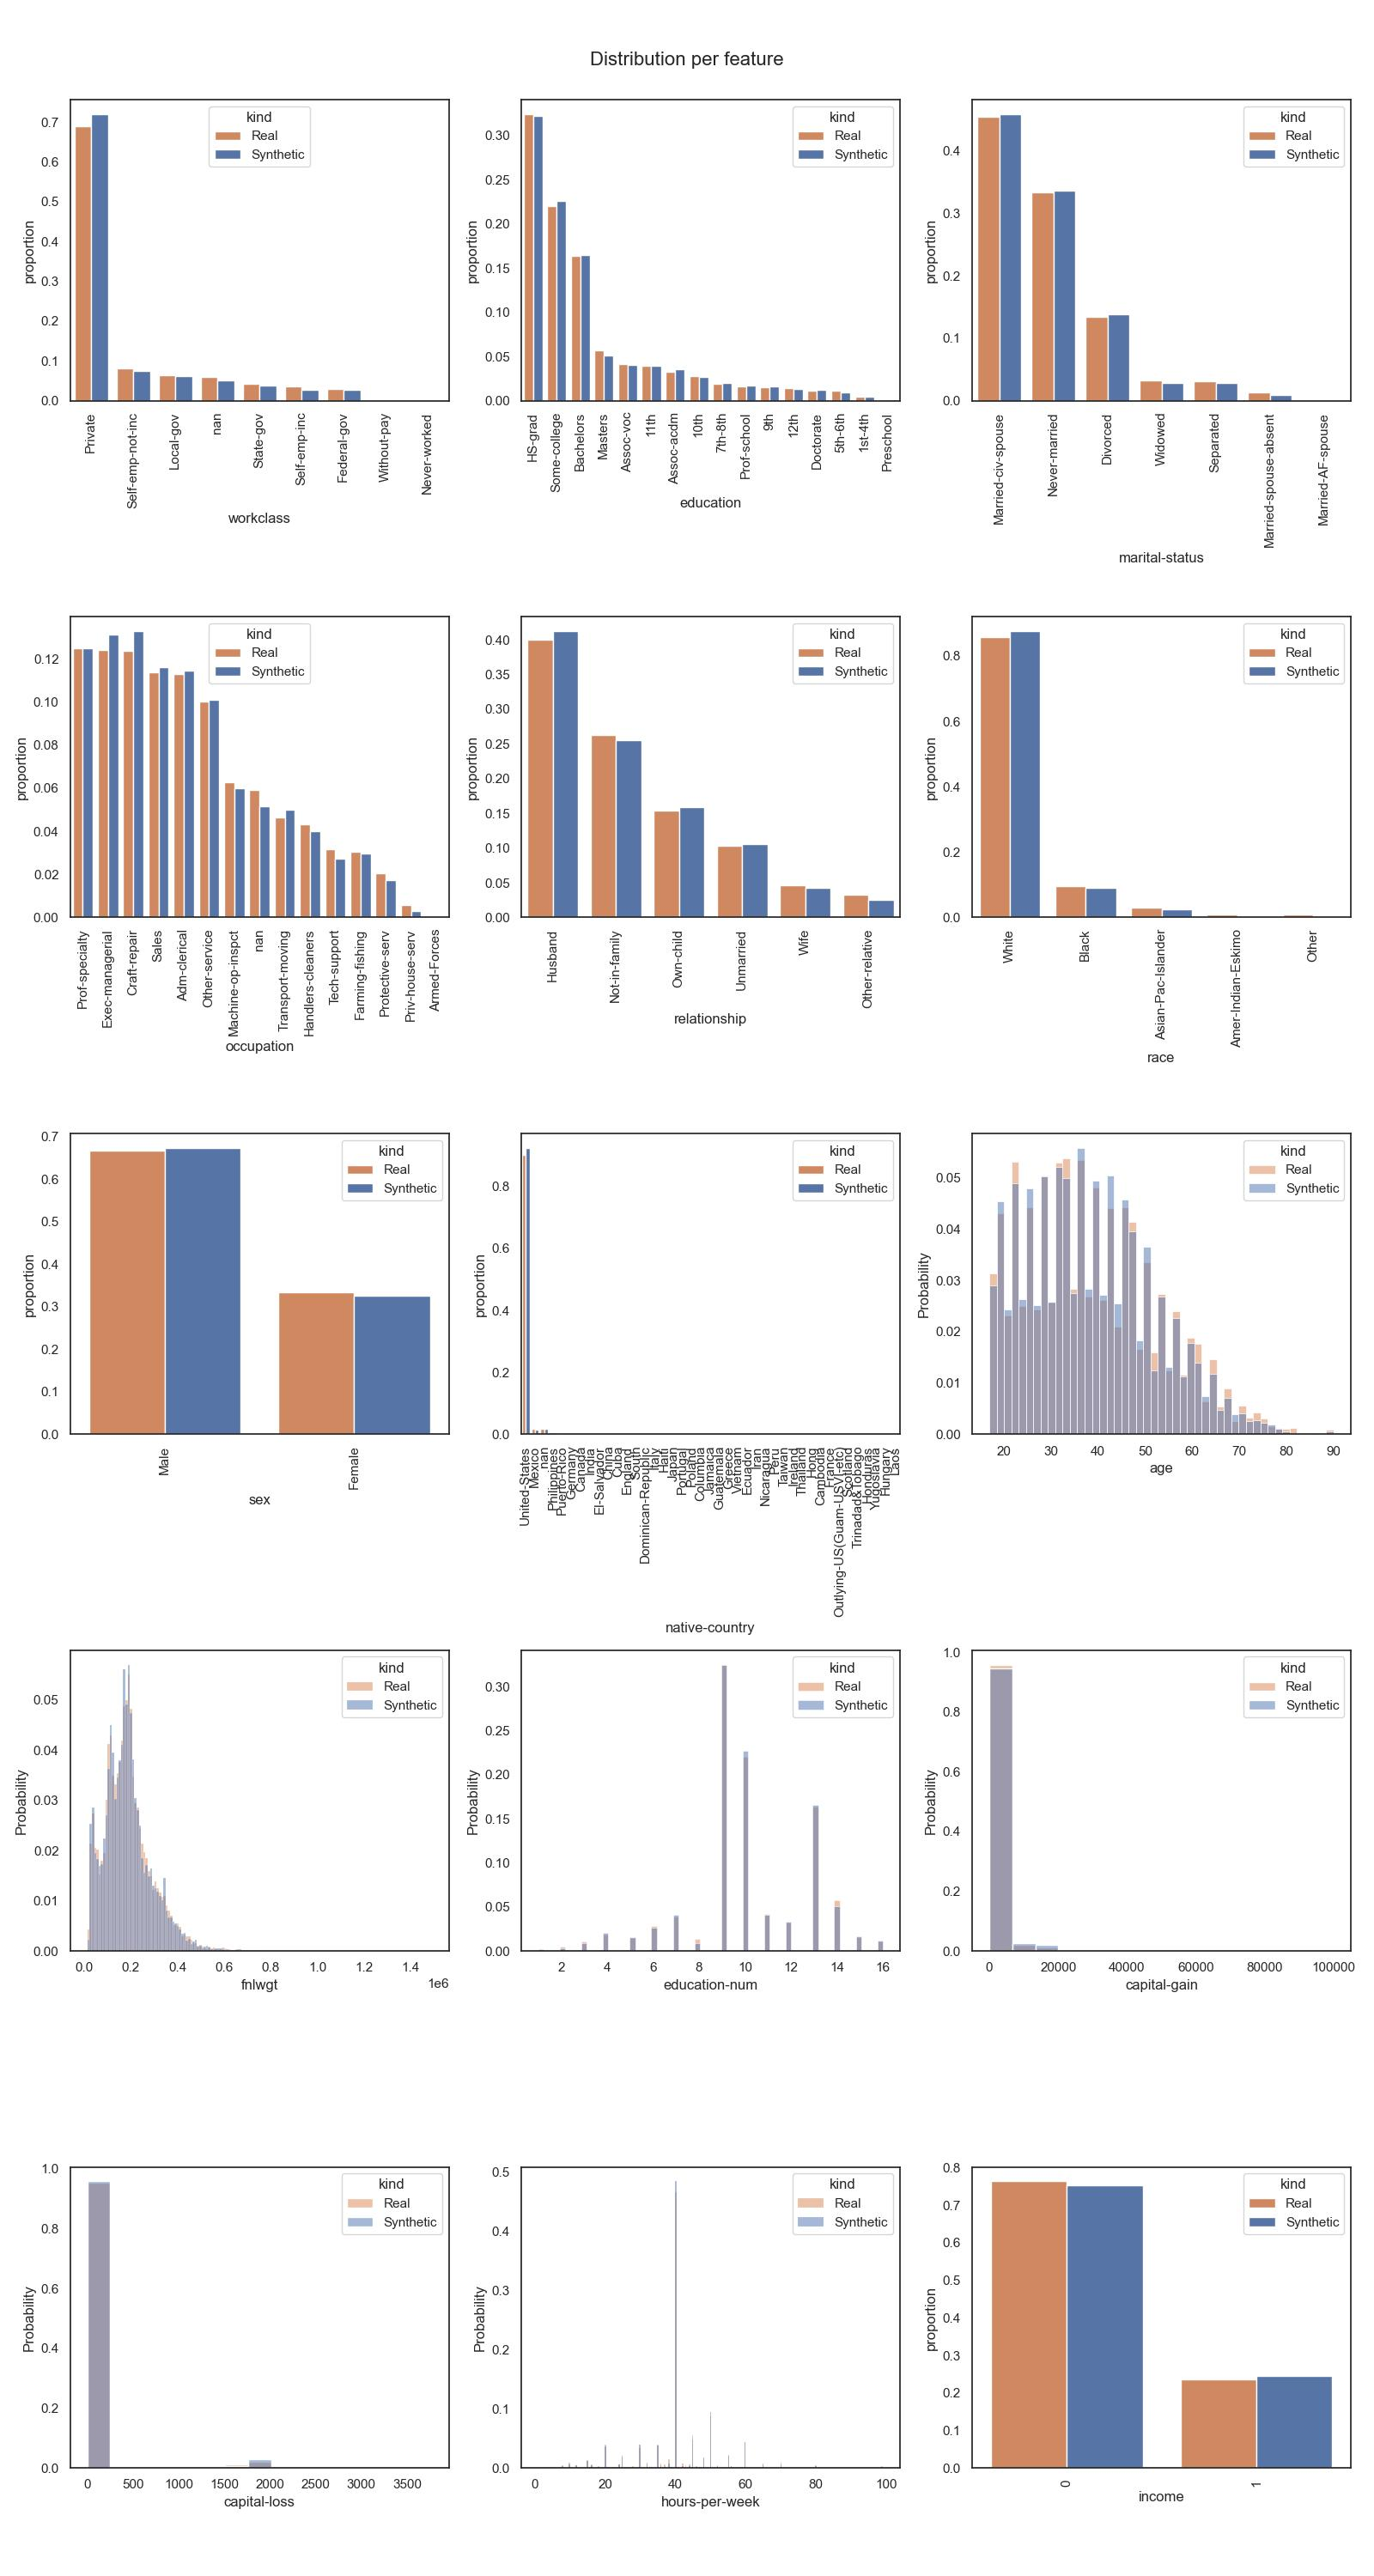
\includegraphics[height=\textheight,width=\linewidth,keepaspectratio]{images/distributions_full/tab-ddpm.jpg}
			\caption{TabDDPM$^{ml}_q$}
		\end{subfigure}
		\hfill
		\begin{subfigure}{0.3\linewidth}
			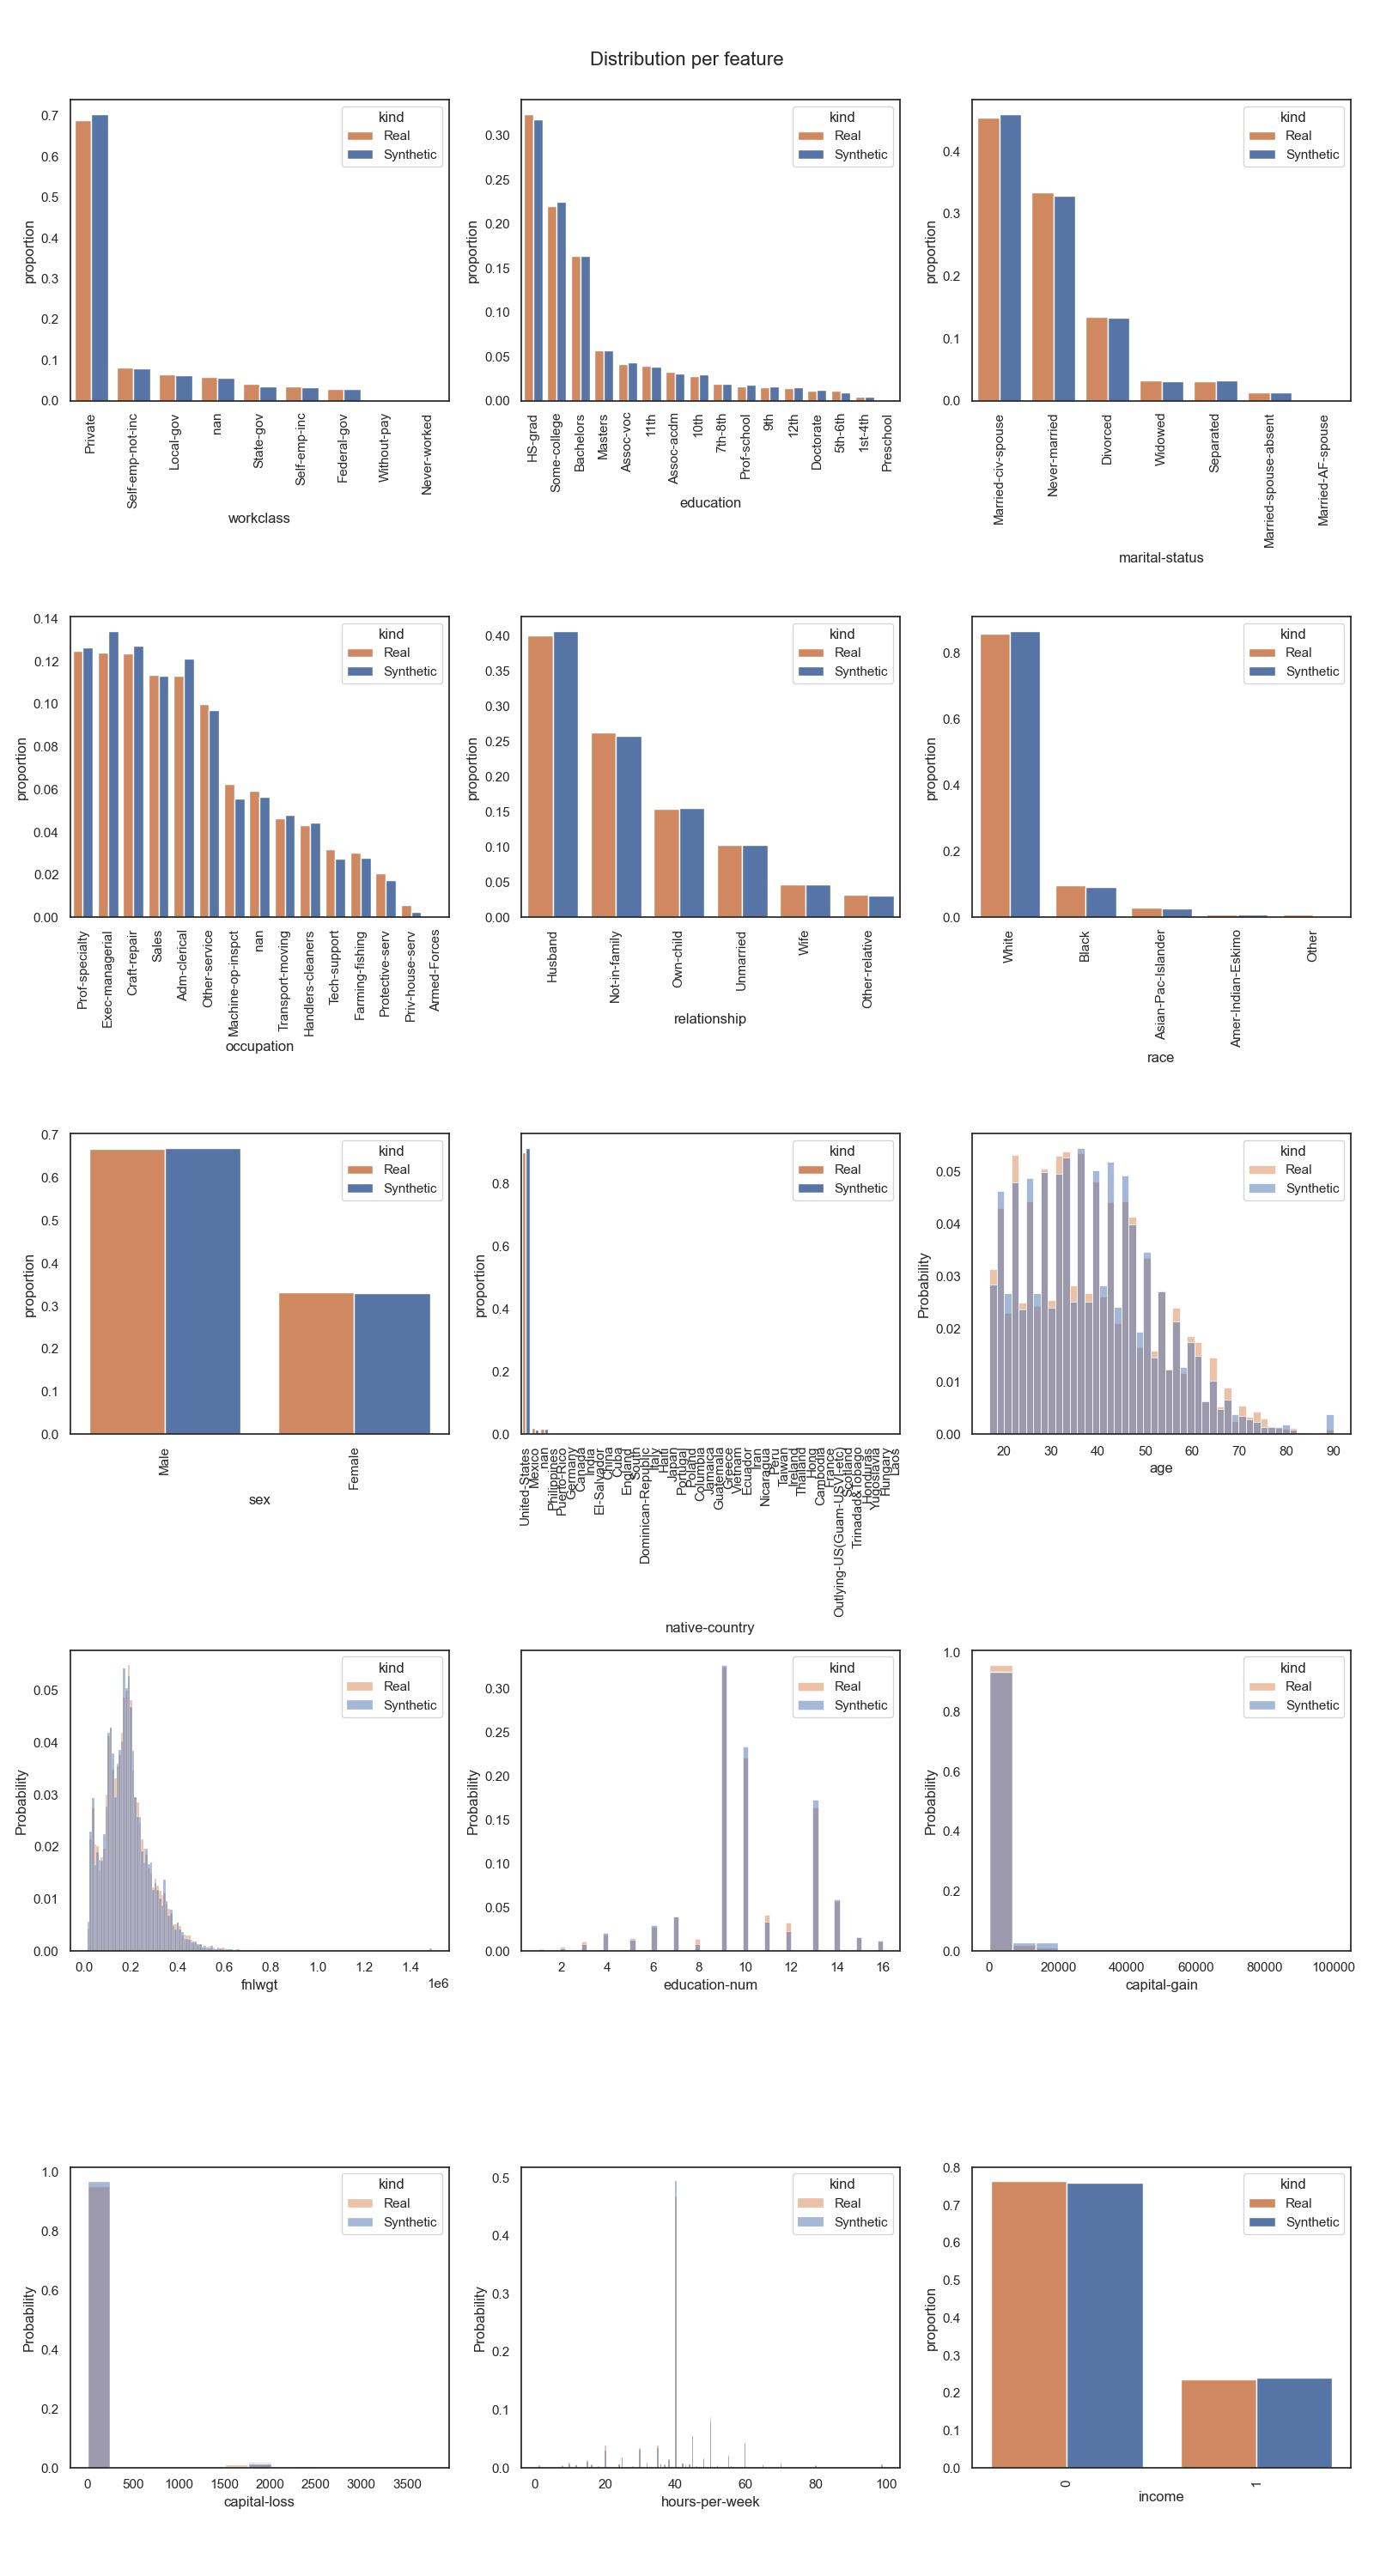
\includegraphics[height=\textheight,width=\linewidth,keepaspectratio]{images/distributions_full/tab-ddpm-simTune.jpg}
			\caption{TabDDPM$^{s}_q$}
		\end{subfigure}
		\hfill
		\begin{subfigure}{0.3\linewidth}
			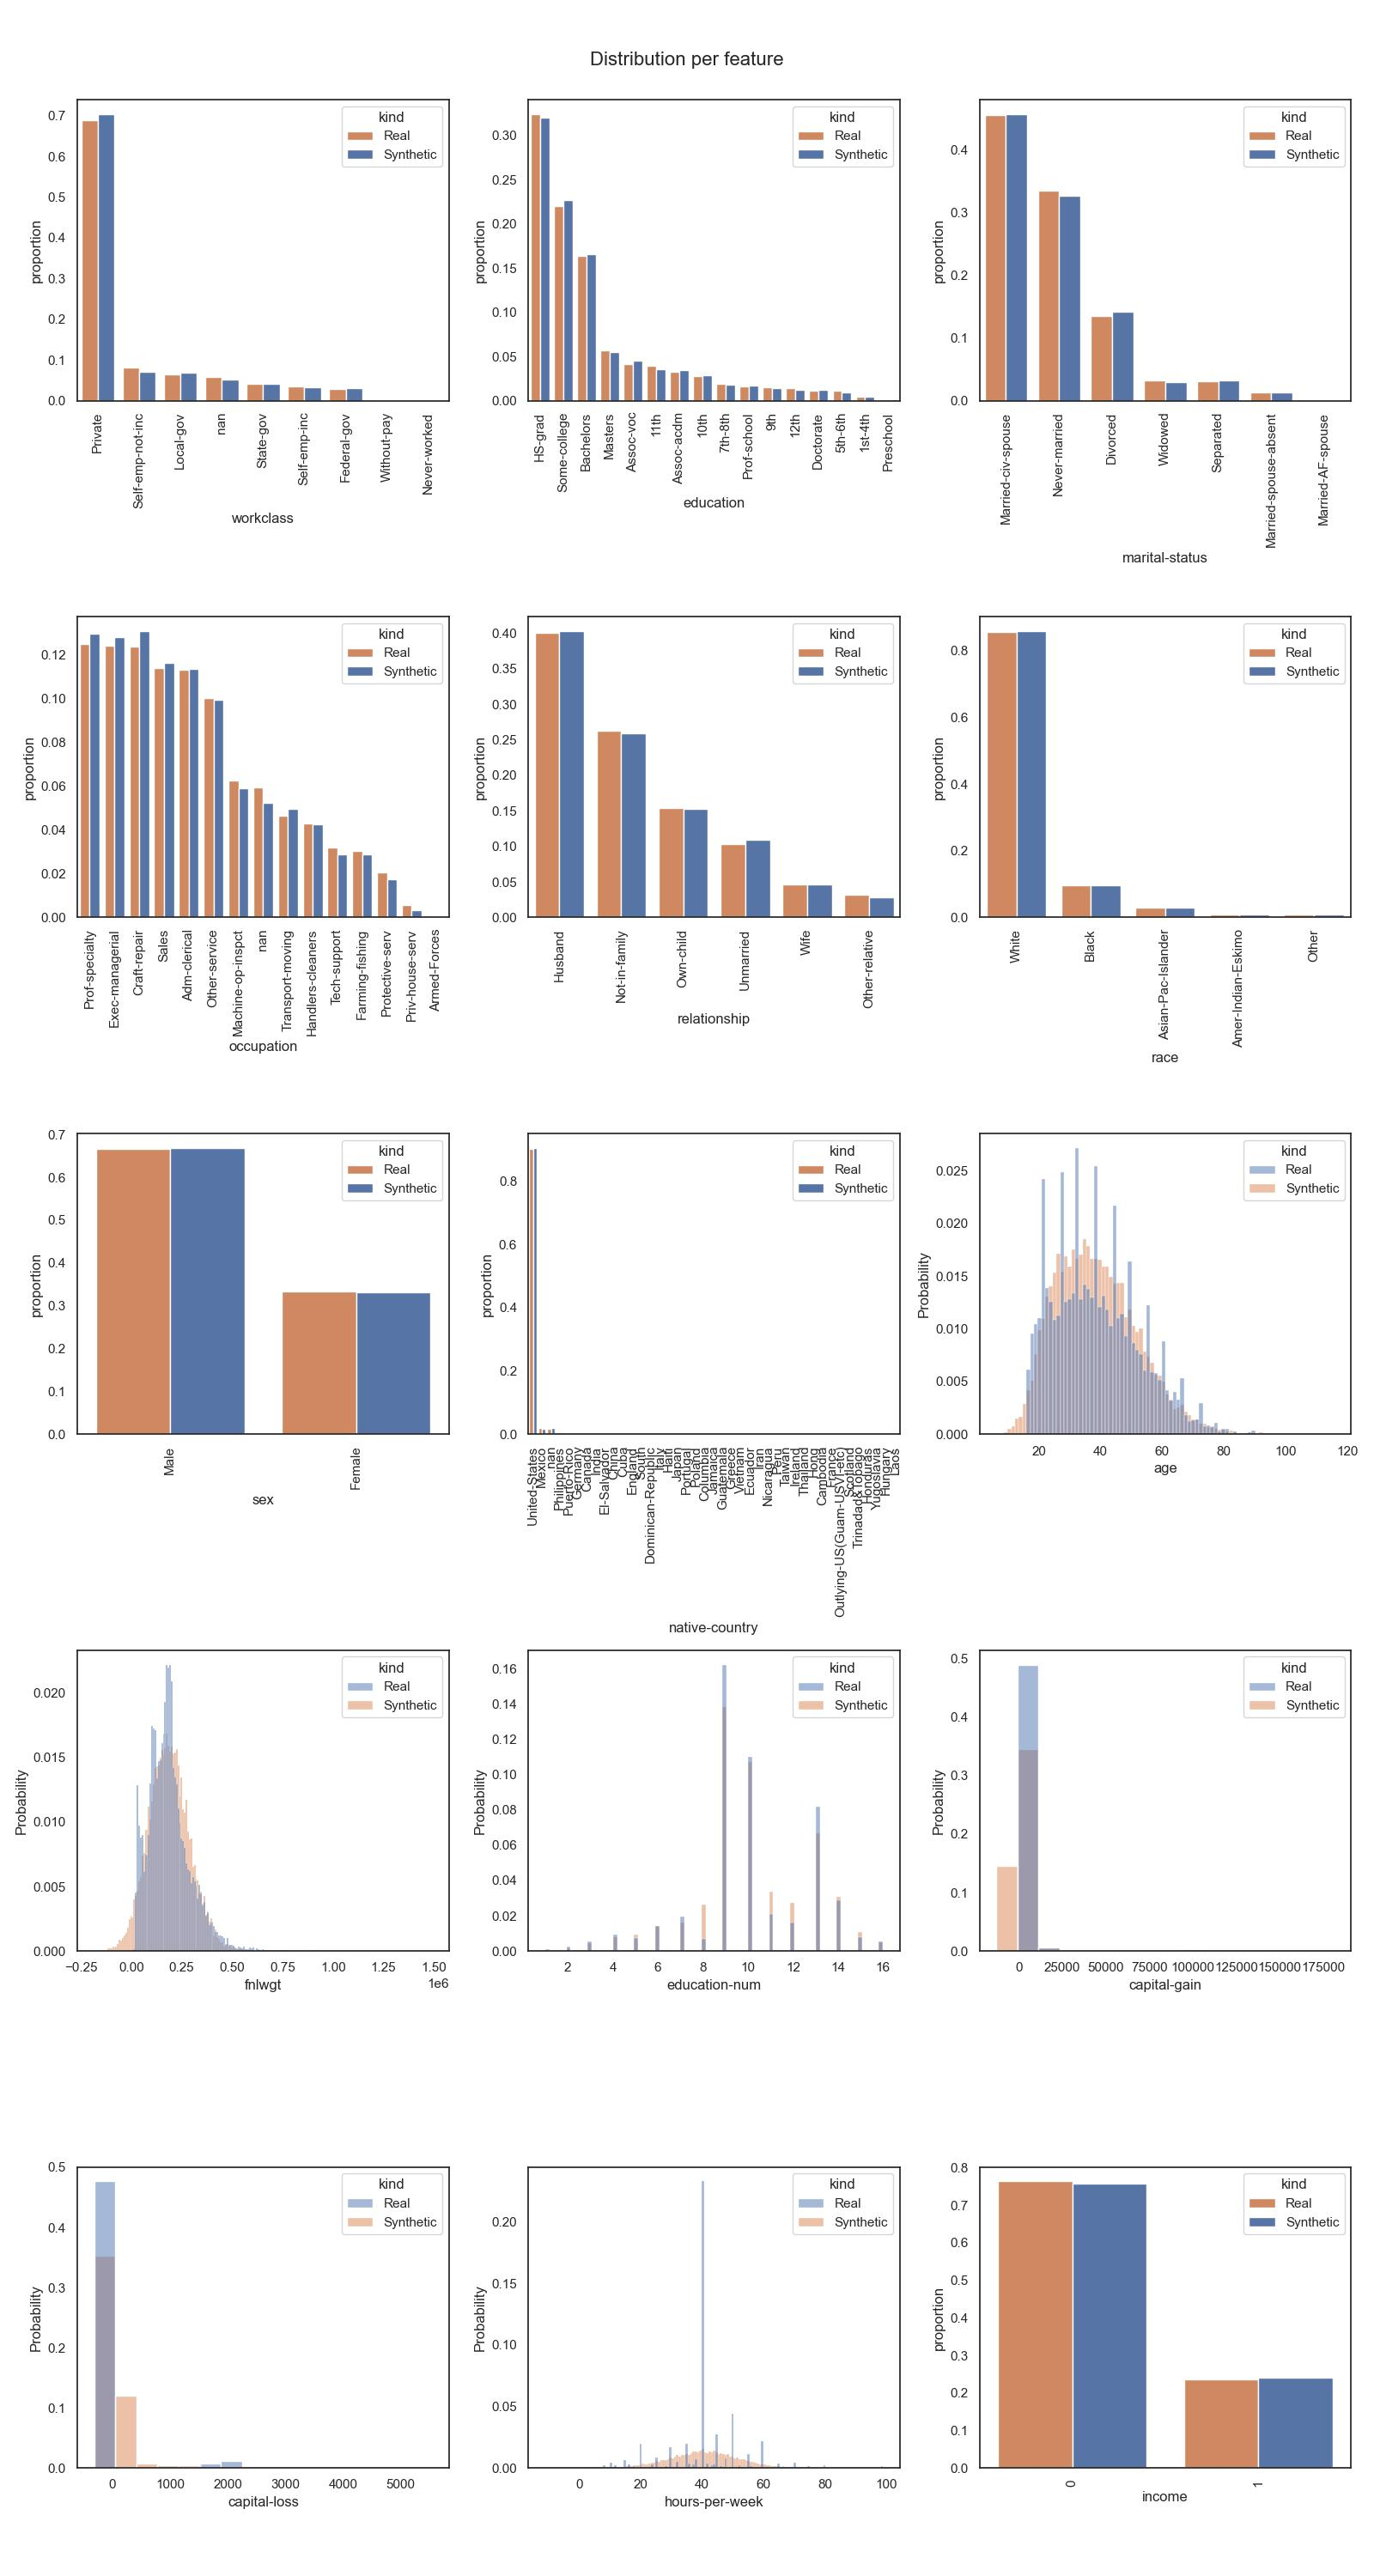
\includegraphics[height=\textheight,width=\linewidth,keepaspectratio]{images/distributions_full/tab-ddpm-simTune-minmax.jpg}
			\caption{TabDDPM$^{s}_m$}
		\end{subfigure}
		\hfill
		\caption{Distribution plots for TabDDPM variations}
		\label{fig_a:dist_3}
	\end{figure}
\end{landscape}
%----------
\newpage
\begin{landscape}
	\begin{figure}[h]
		\centering
		\hfill
		\begin{subfigure}{0.3\linewidth}
			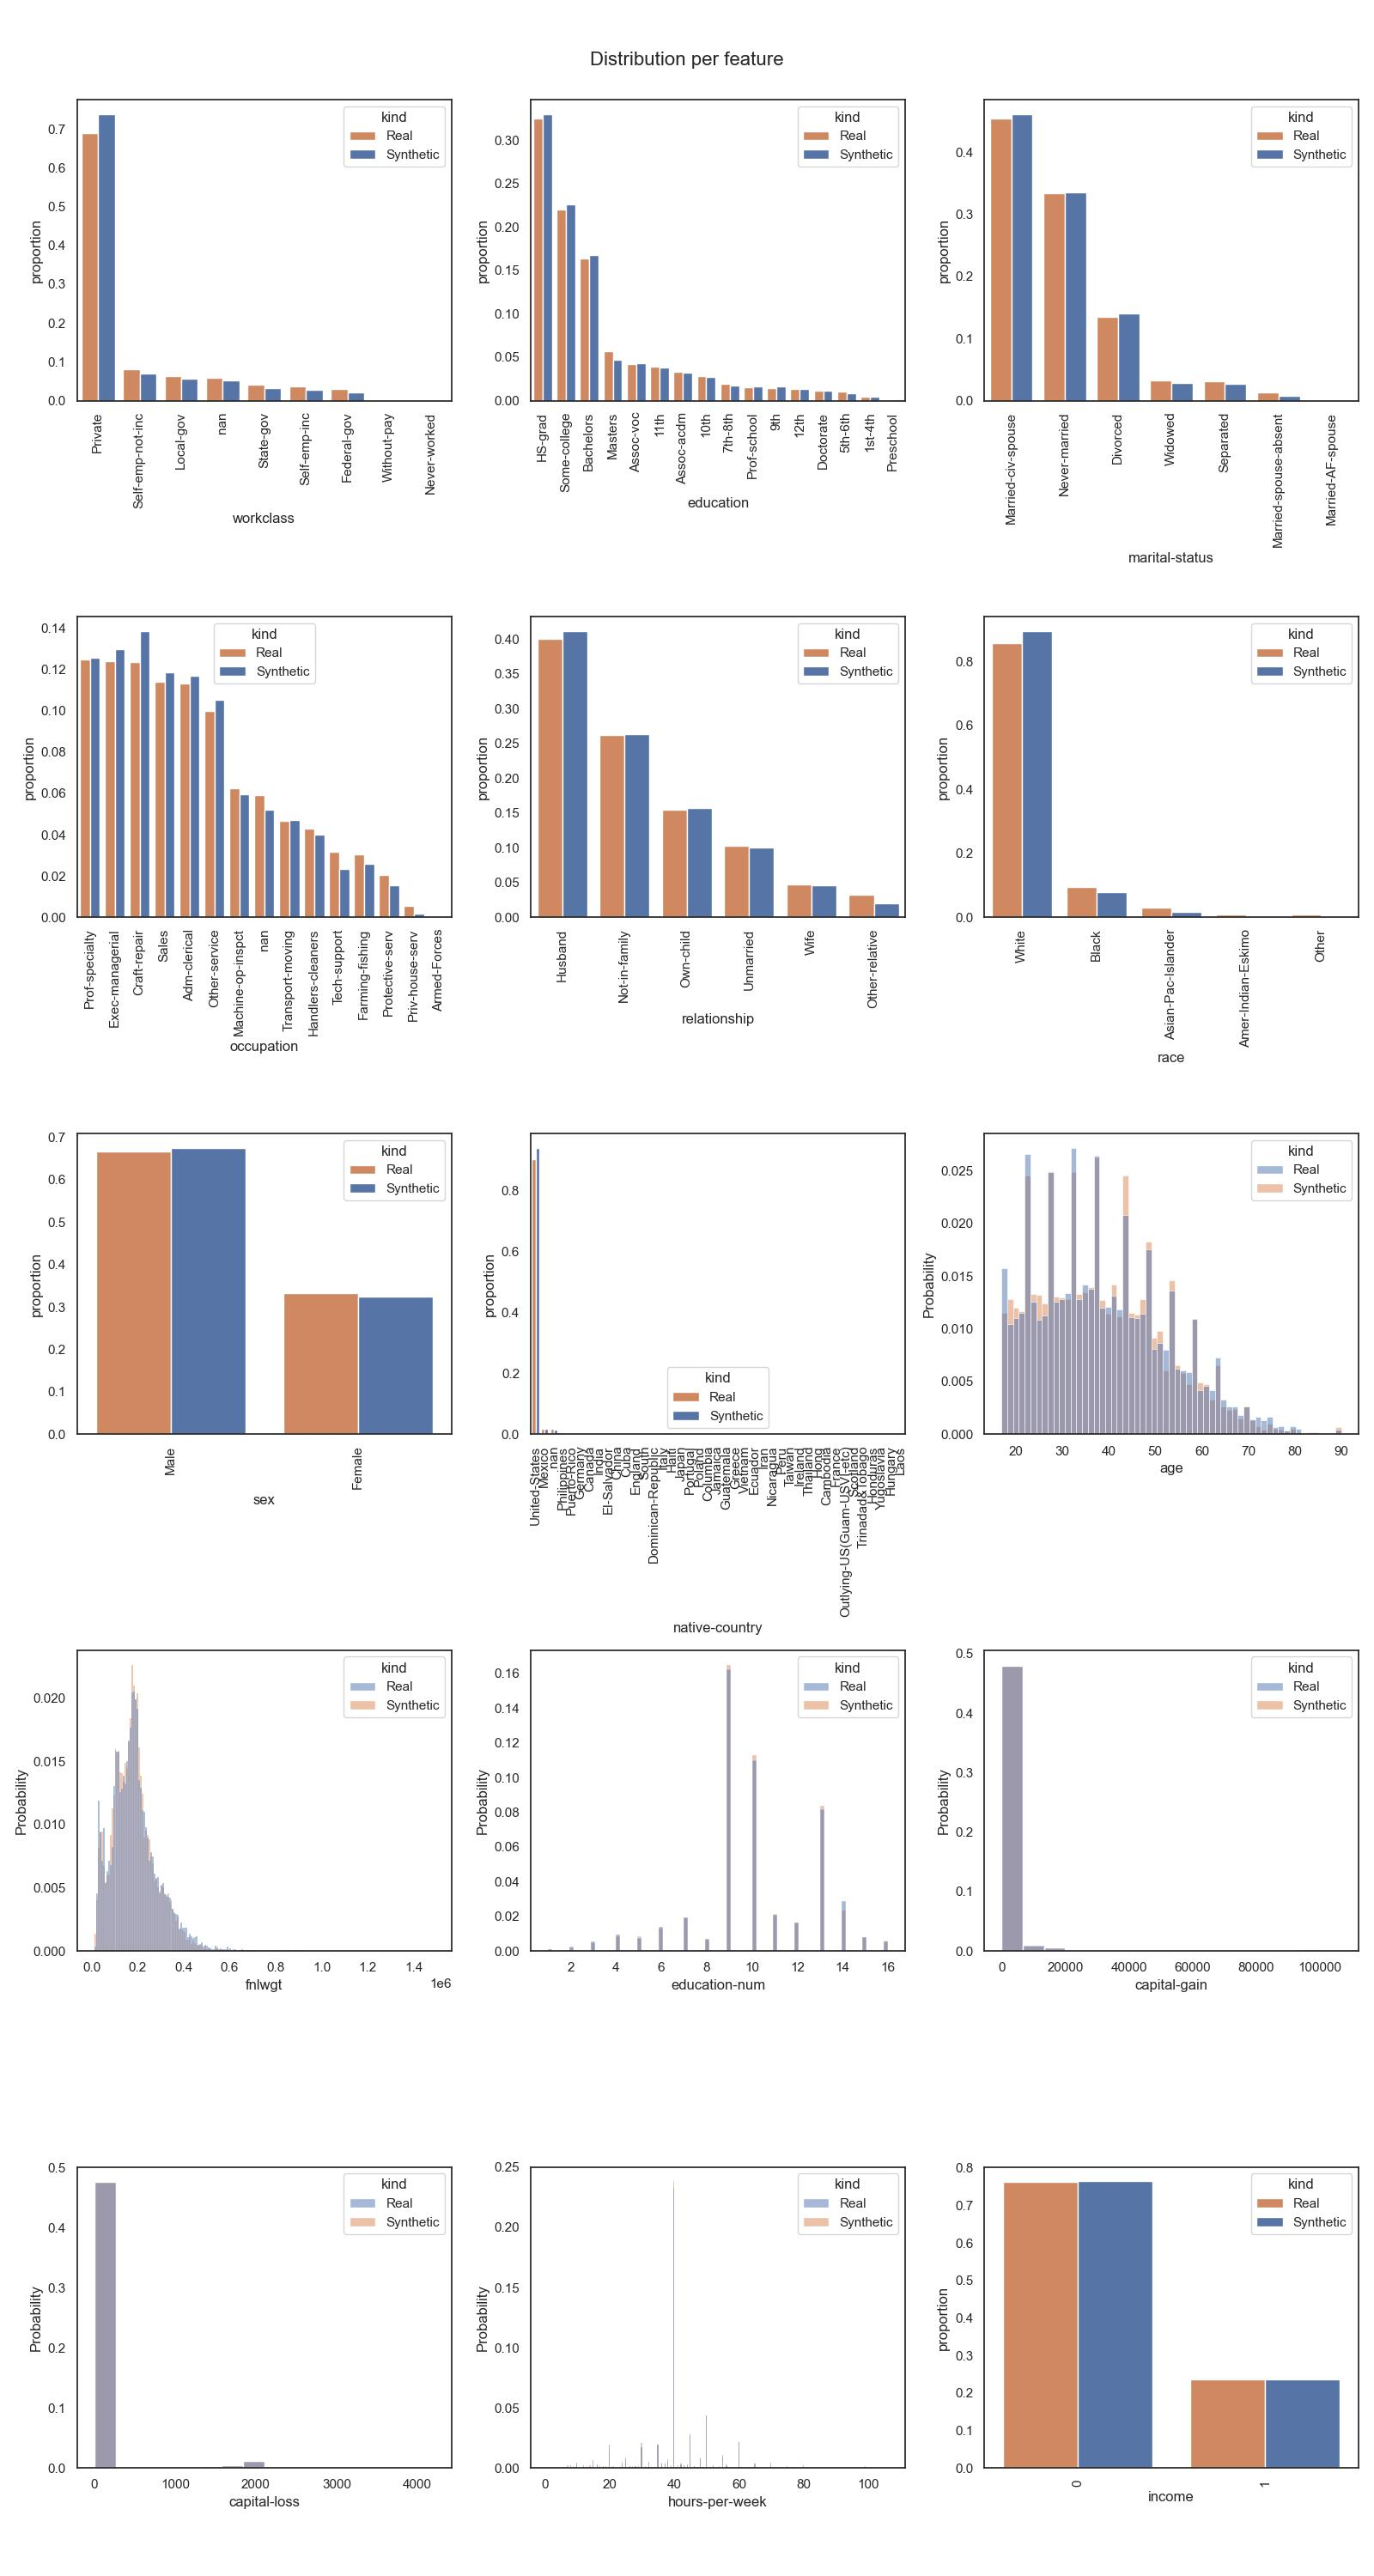
\includegraphics[height=\textheight,width=\linewidth,keepaspectratio]{images/distributions_full/tab-ddpm-bgm.jpg}
			\caption{TabDDPM-BGM$^{ml}_q$}
		\end{subfigure}
		\hfill
		\begin{subfigure}{0.3\linewidth}
			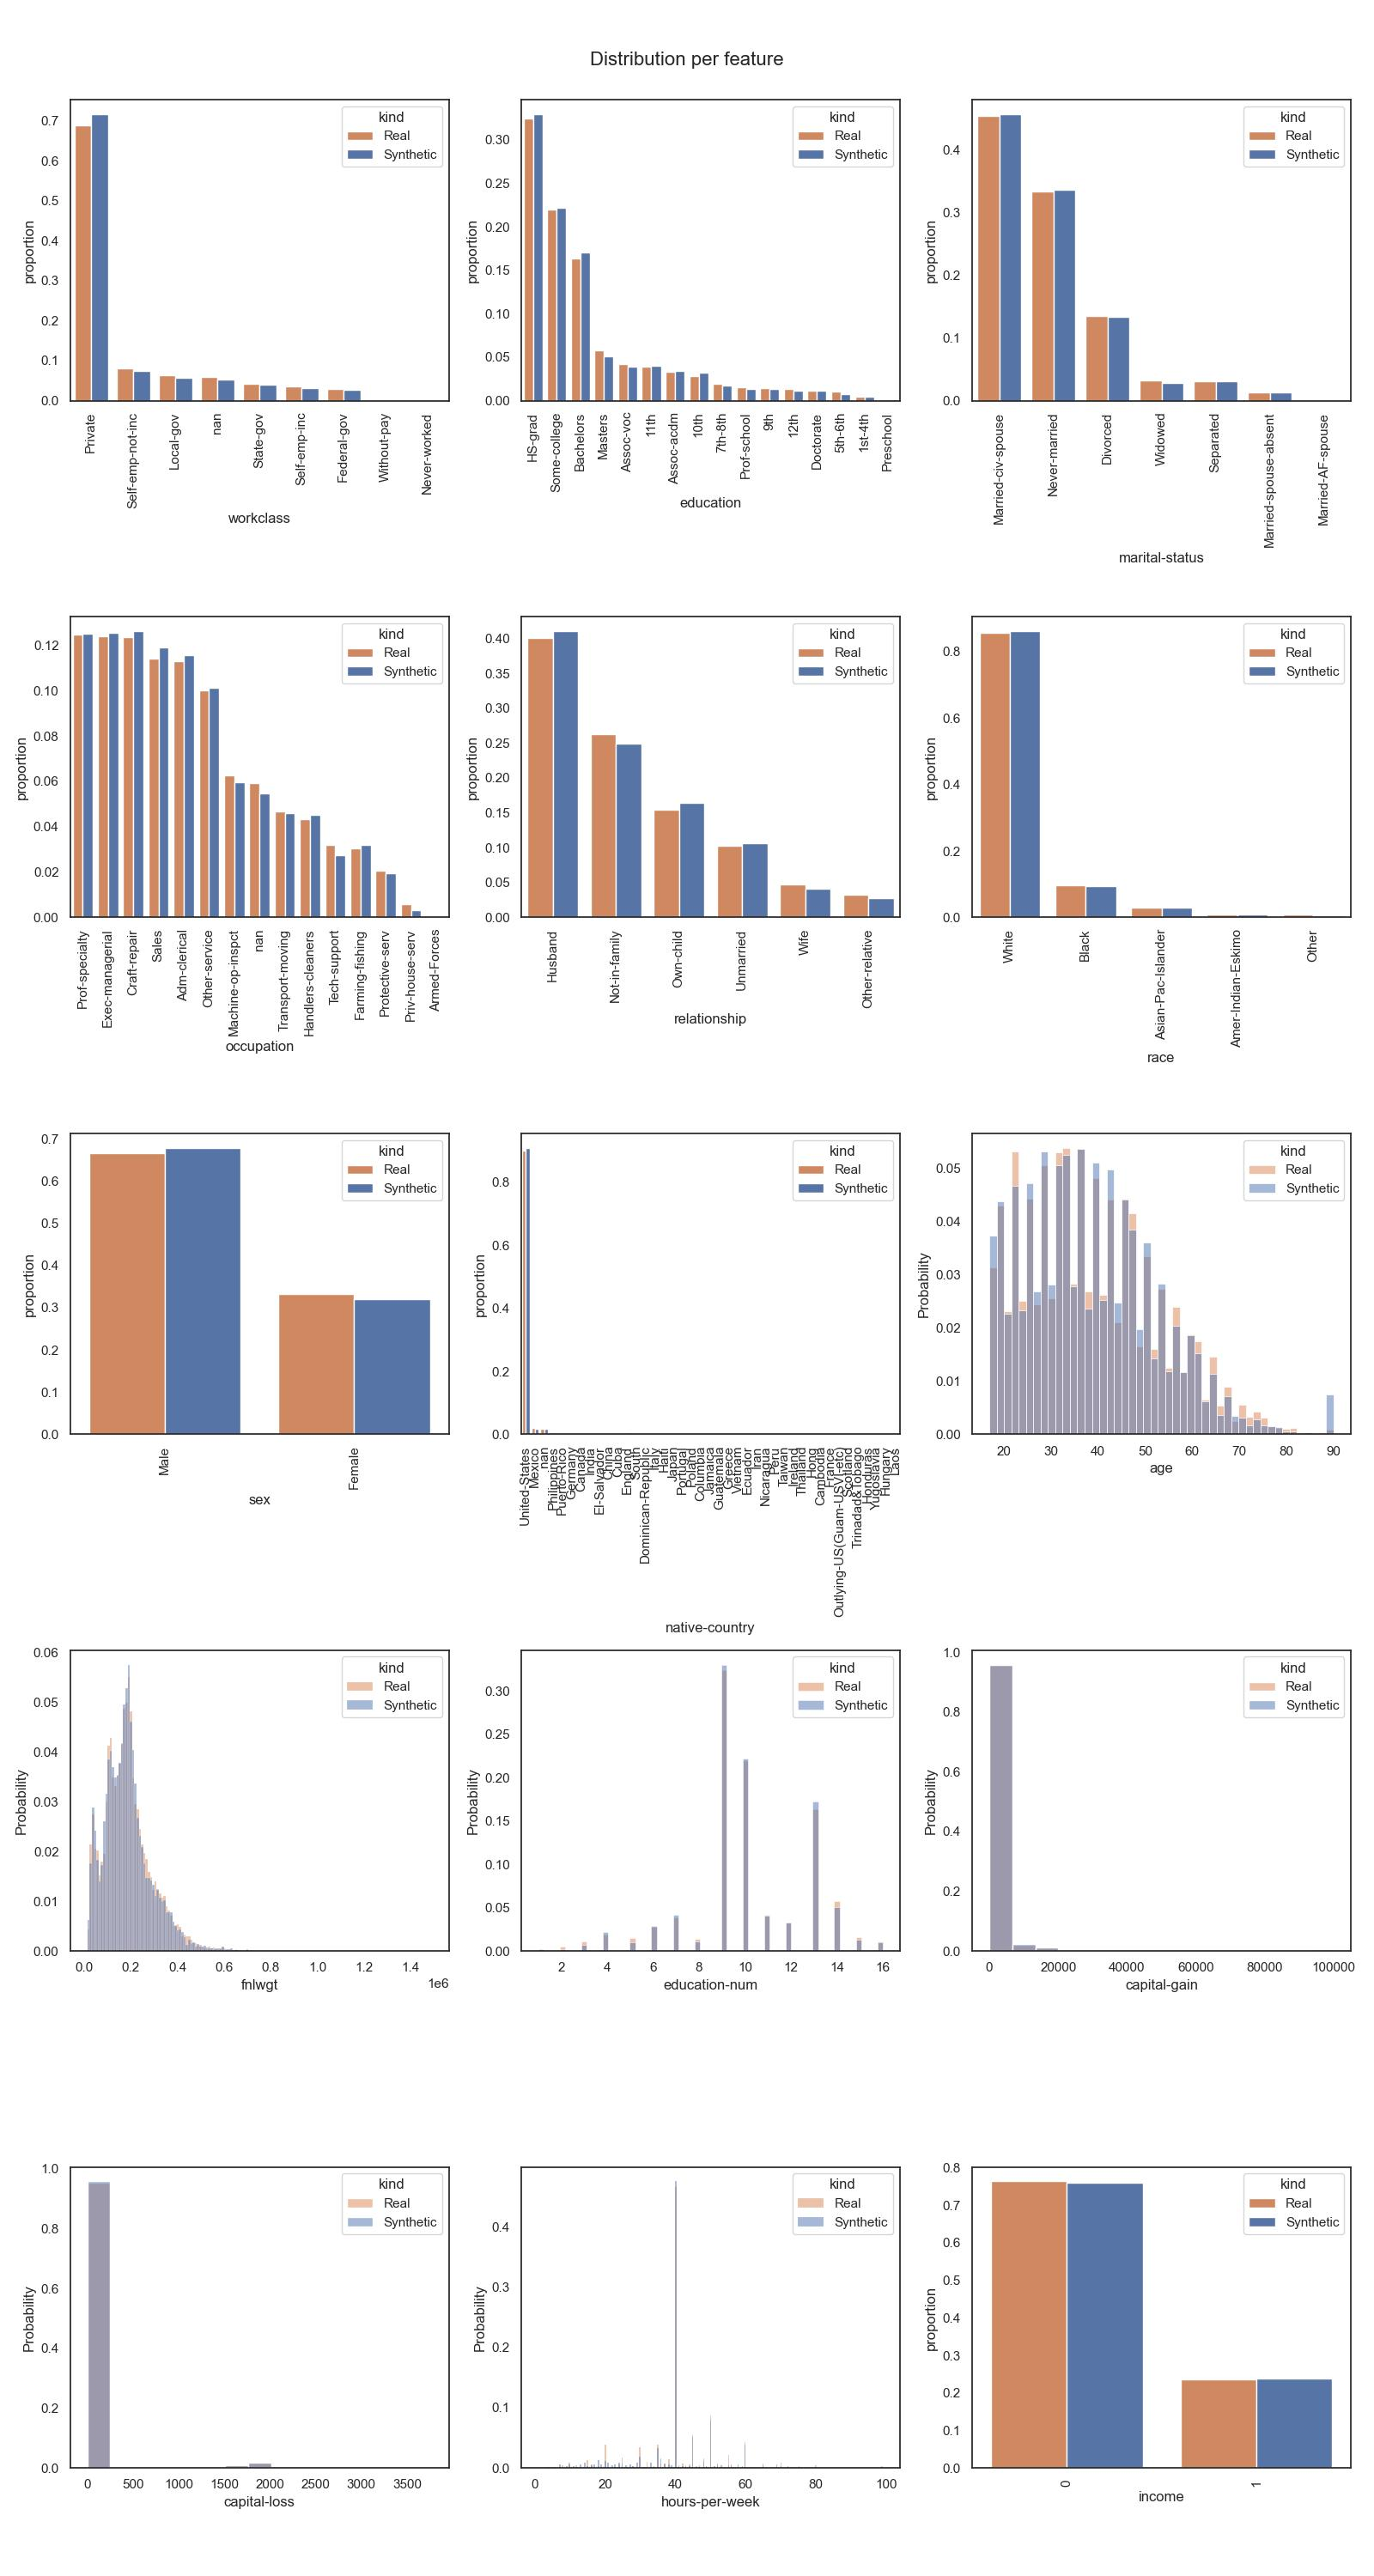
\includegraphics[height=\textheight,width=\linewidth,keepaspectratio]{images/distributions_full/tab-ddpm-bgm-simTune.jpg}
			\caption{TabDDPM-BGM$^{s}_q$}
		\end{subfigure}
		\hfill
		\begin{subfigure}{0.3\linewidth}
			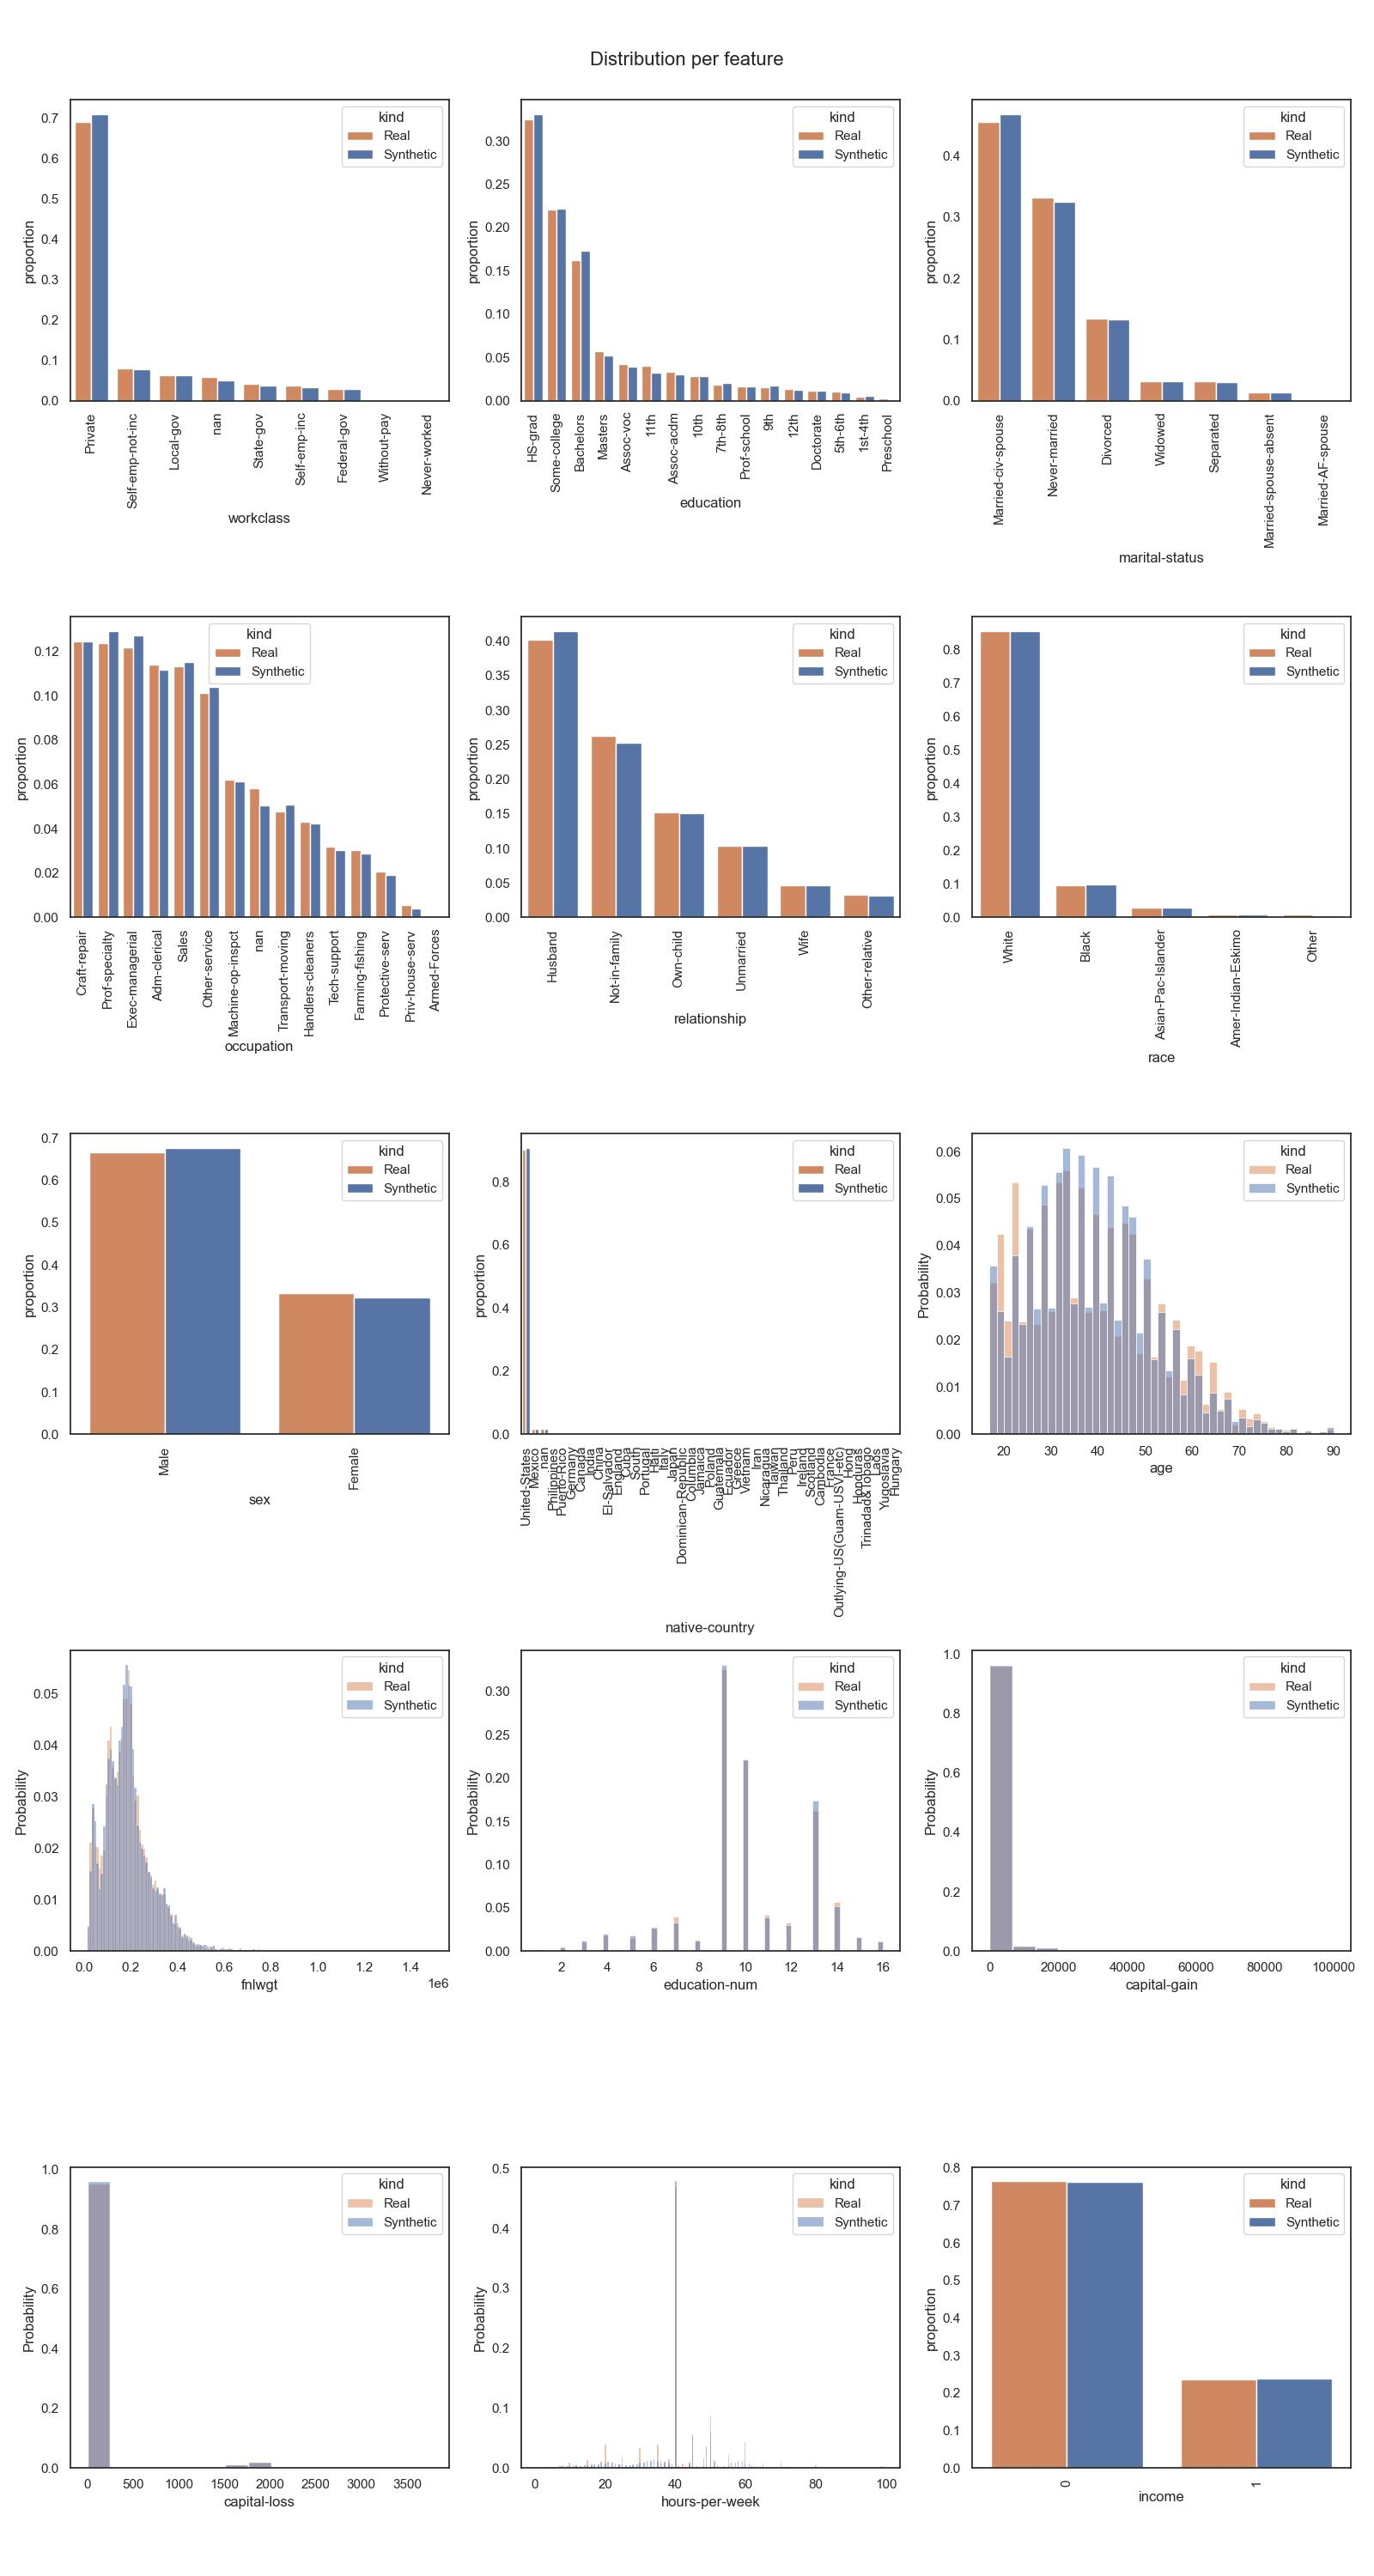
\includegraphics[height=\textheight,width=\linewidth,keepaspectratio]{images/distributions_full/tab-ddpm-bgm-simTune-minmax.jpg}
			\caption{TabDDPM-BGM$^{s}_m$}
		\end{subfigure}
		\caption{Distribution plots for TabDDPM-BGM variations}
		\label{fig_a:dist_4}
	\end{figure}
\end{landscape}
%----------
\newpage
\begin{landscape}
	\begin{figure}[h]
		\centering
		\hfill
		\begin{subfigure}{0.4\linewidth}
			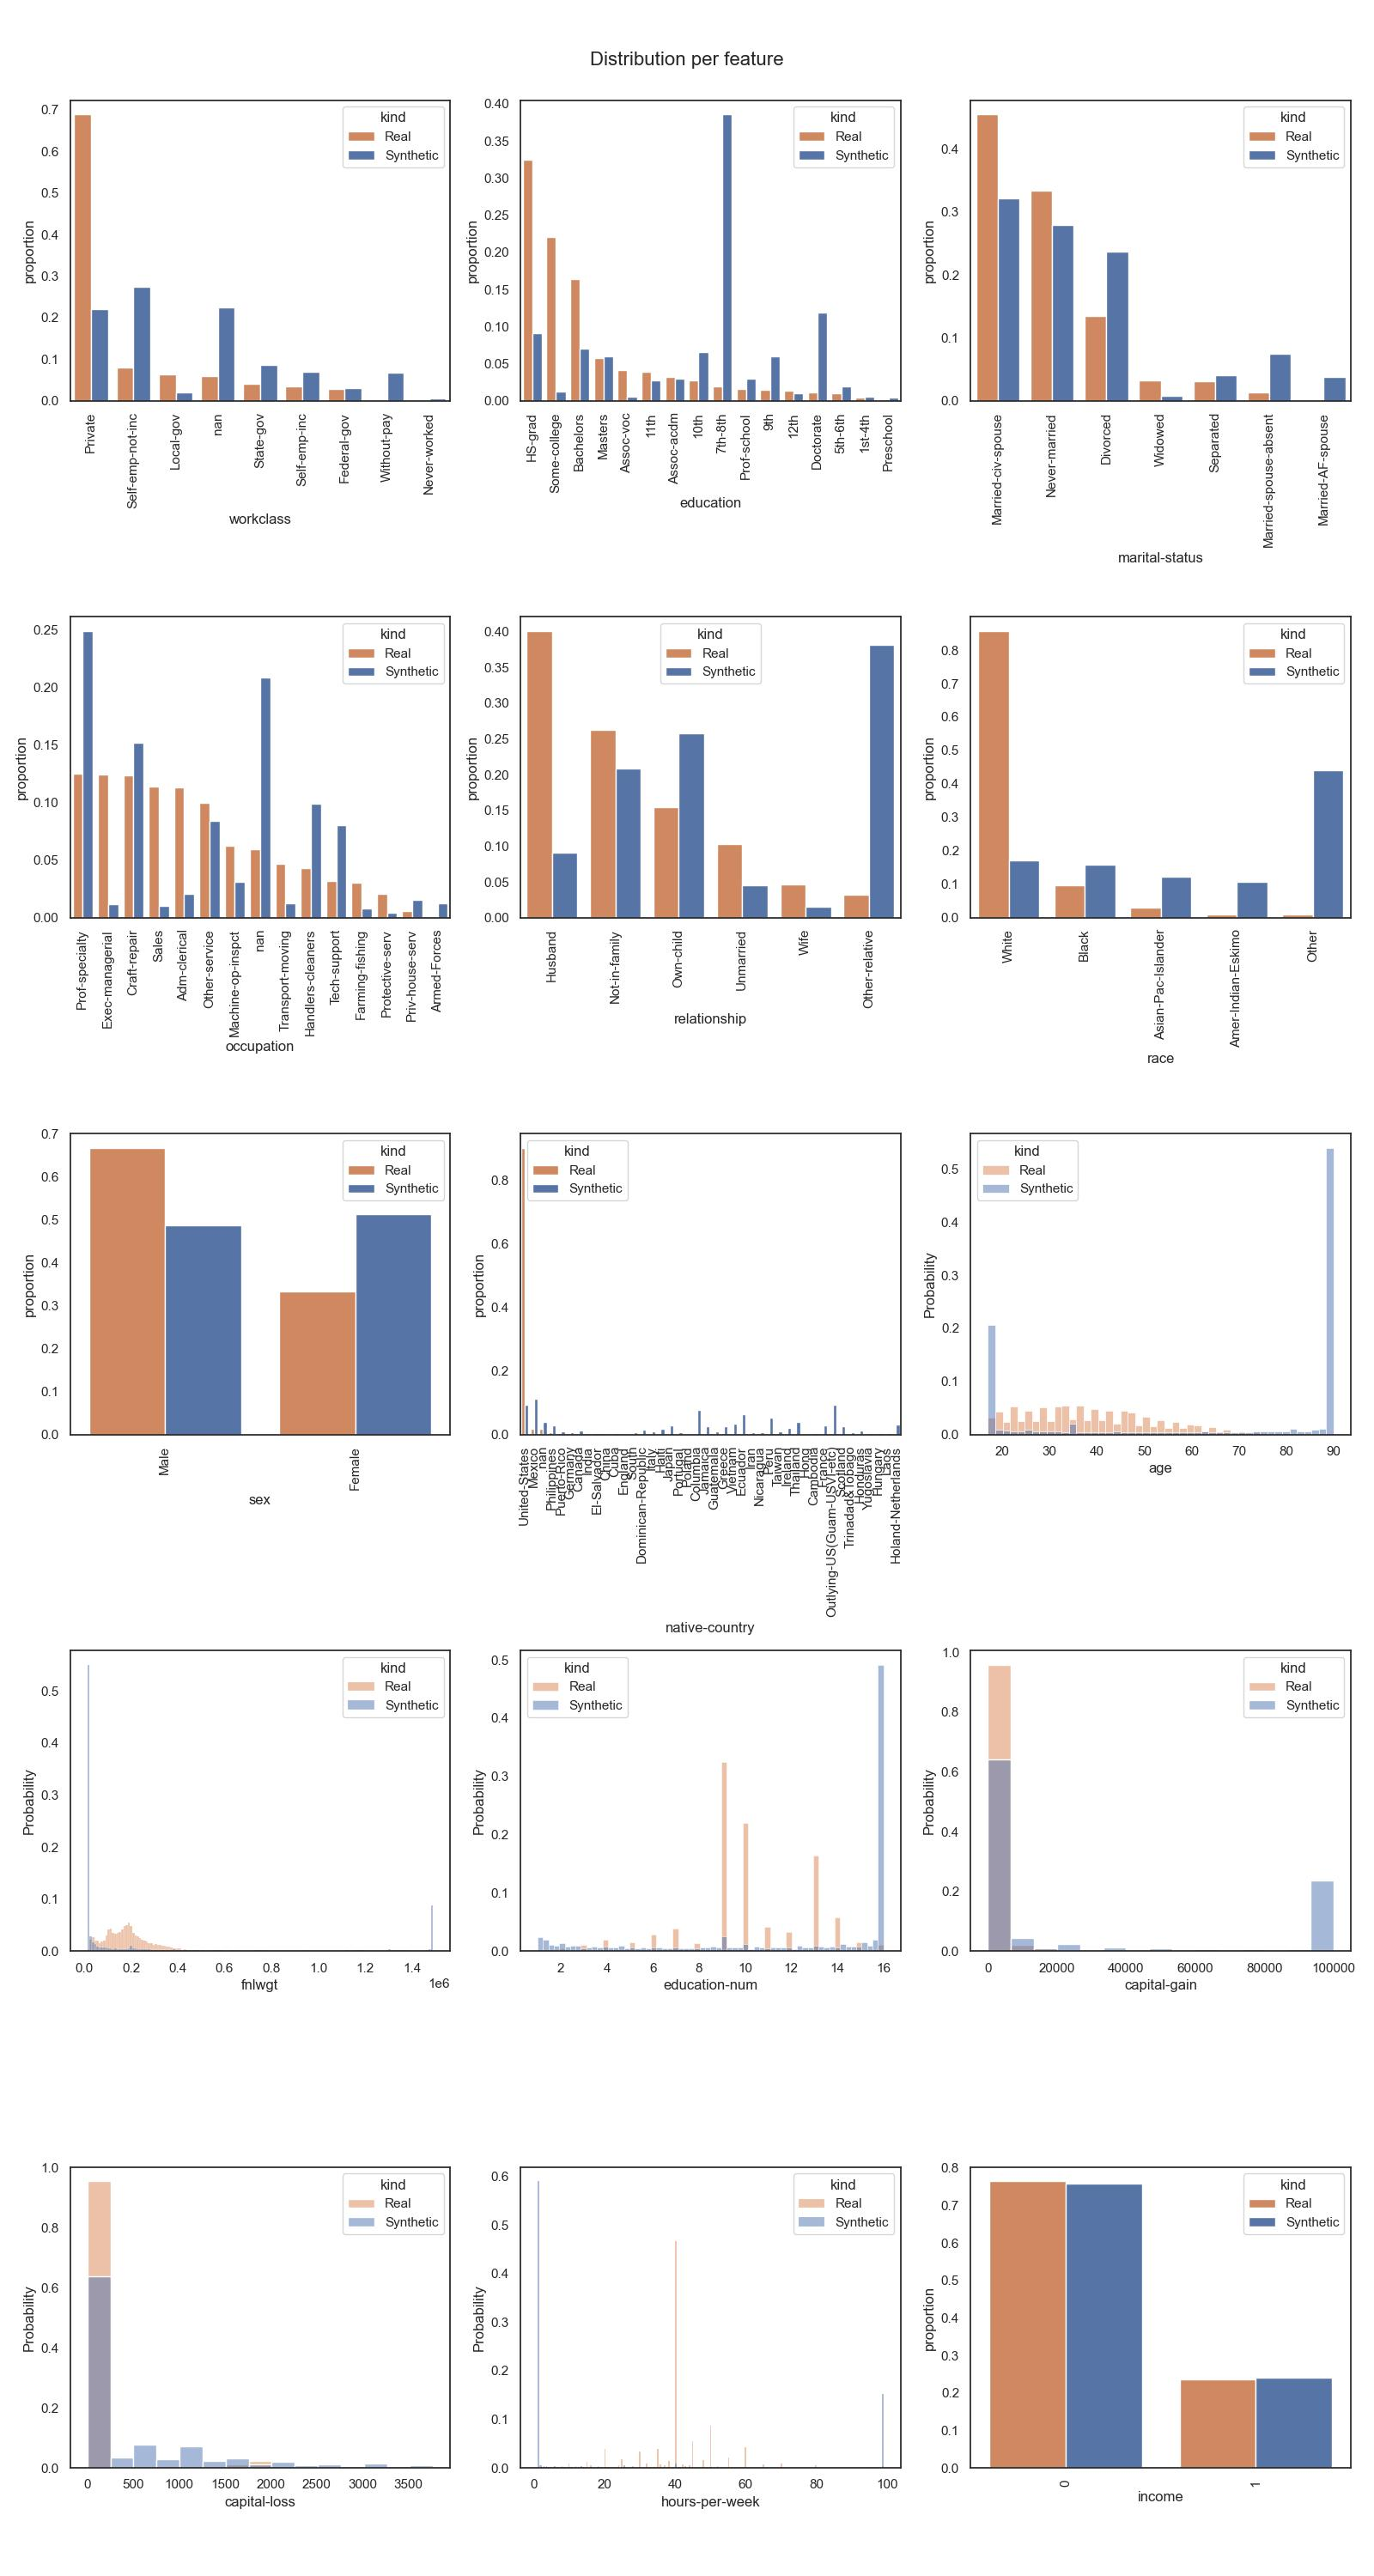
\includegraphics[height=\textheight,width=\linewidth,keepaspectratio]{images/distributions_full/tab-ddpm-ft.jpg}
			\caption{TabDDPM-FT$^{ml}_q$}
		\end{subfigure}
		\hfill
		\begin{subfigure}{0.4\linewidth}
			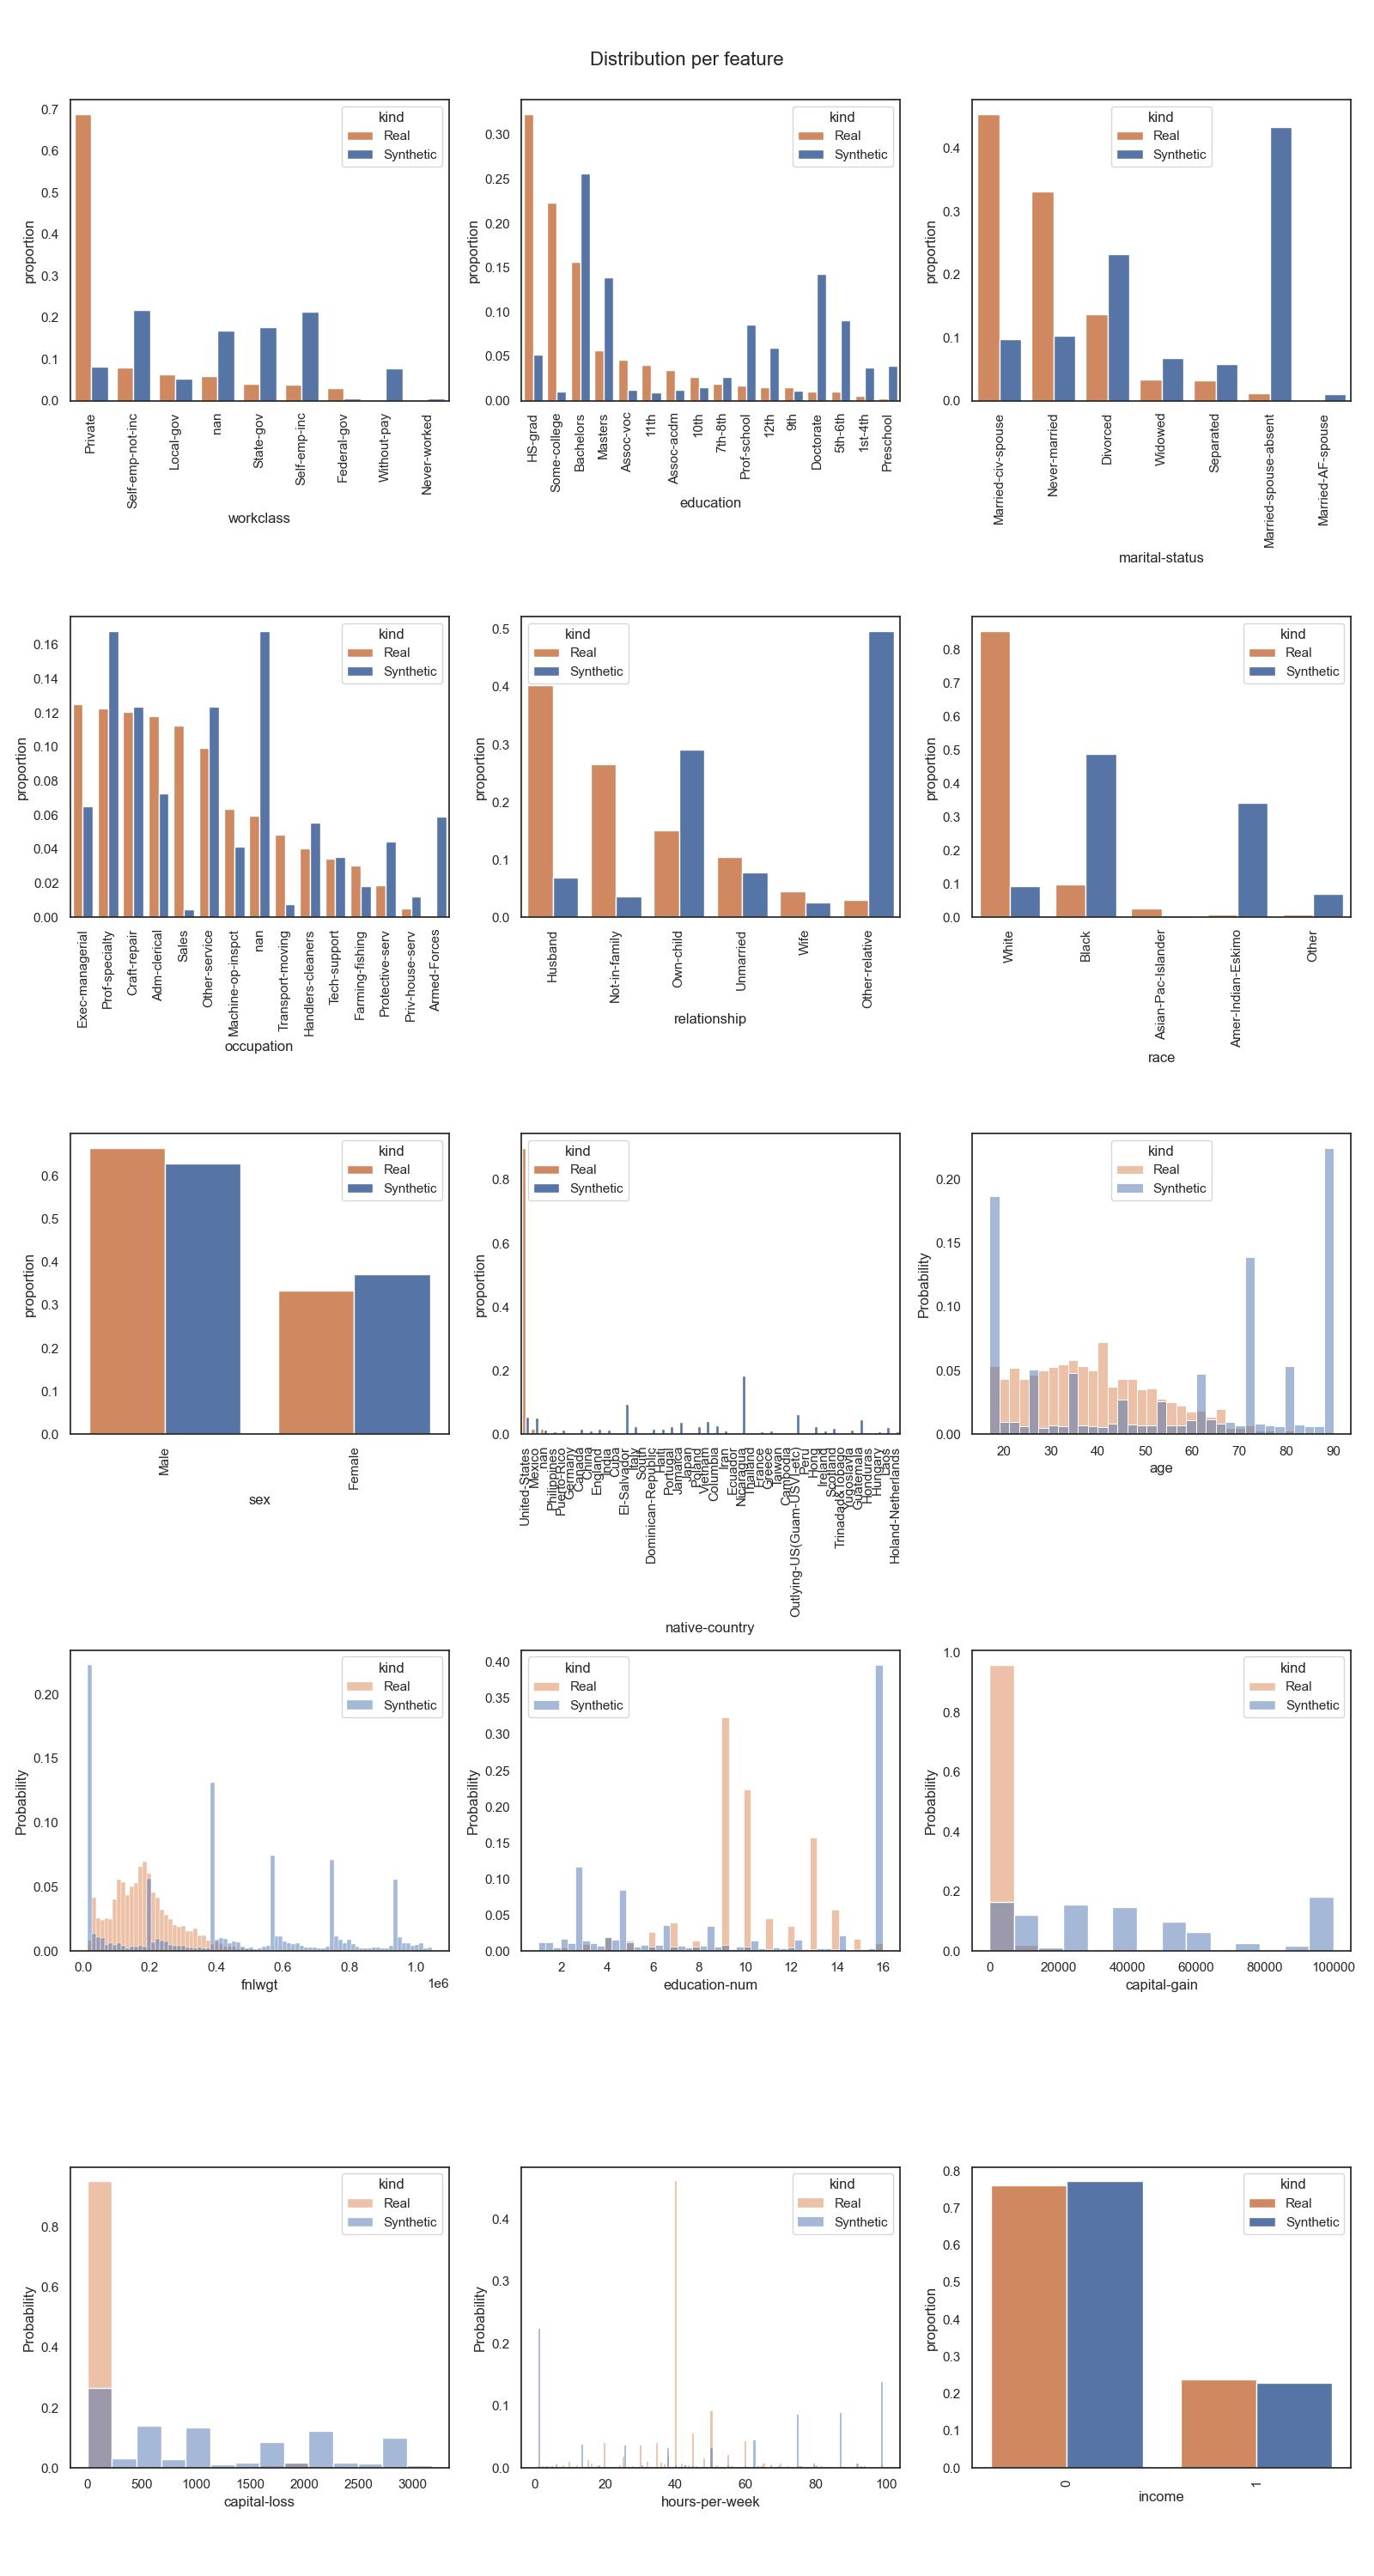
\includegraphics[height=\textheight,width=\linewidth,keepaspectratio]{images/distributions_full/tab-ddpm-ft-simTune.jpg}
			\caption{TabDDPM-FT$^{ml}_q$}
		\end{subfigure}
		\caption{Distribution plots for TabDDPM-FT variations}
		\label{fig_a:dist_5}
	\end{figure}
\end{landscape}



%-------------


\subsection[]{Cumulative Distribution Plots}
\label{A:cumsum}
%----------
\newpage
\begin{landscape}
	\begin{figure}[h]
		\centering
		\hfill
		\begin{subfigure}{0.3\linewidth}
			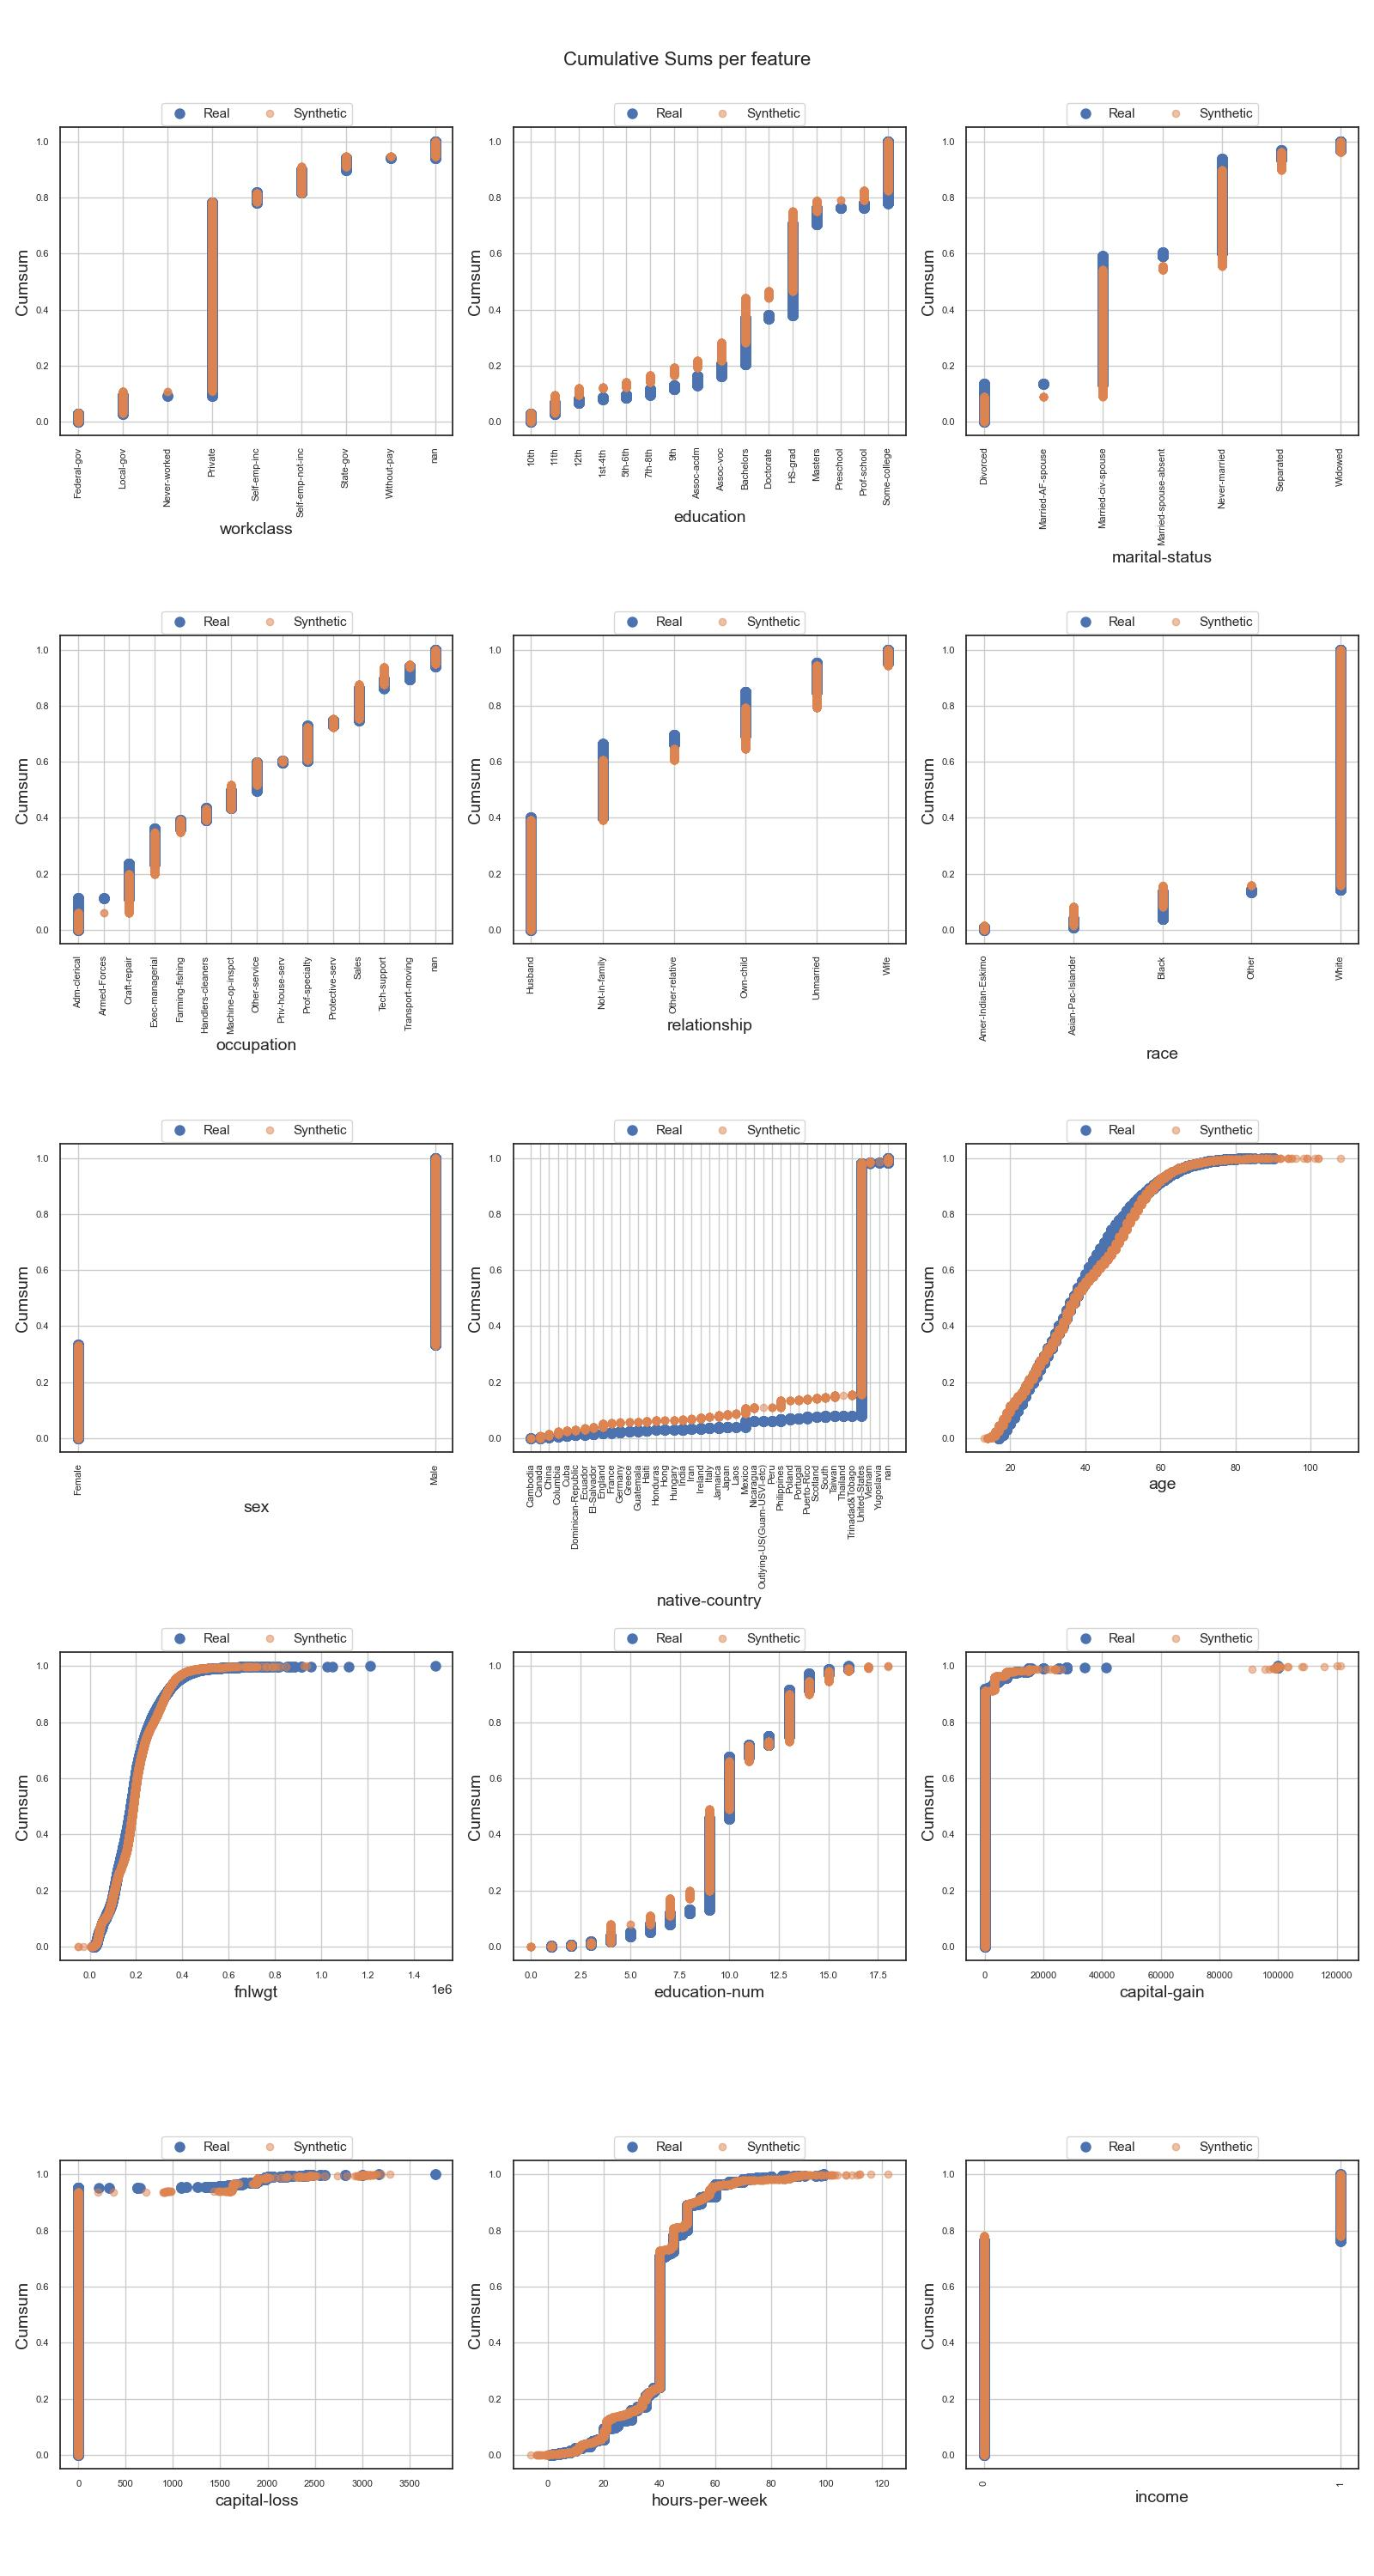
\includegraphics[height=\textheight,width=\linewidth,keepaspectratio]{images/cumsums/ctabgan.jpg}
			\caption{CTABGAN$^{ml}$}
		\end{subfigure}
		\hfill
		\begin{subfigure}{0.3\linewidth}
			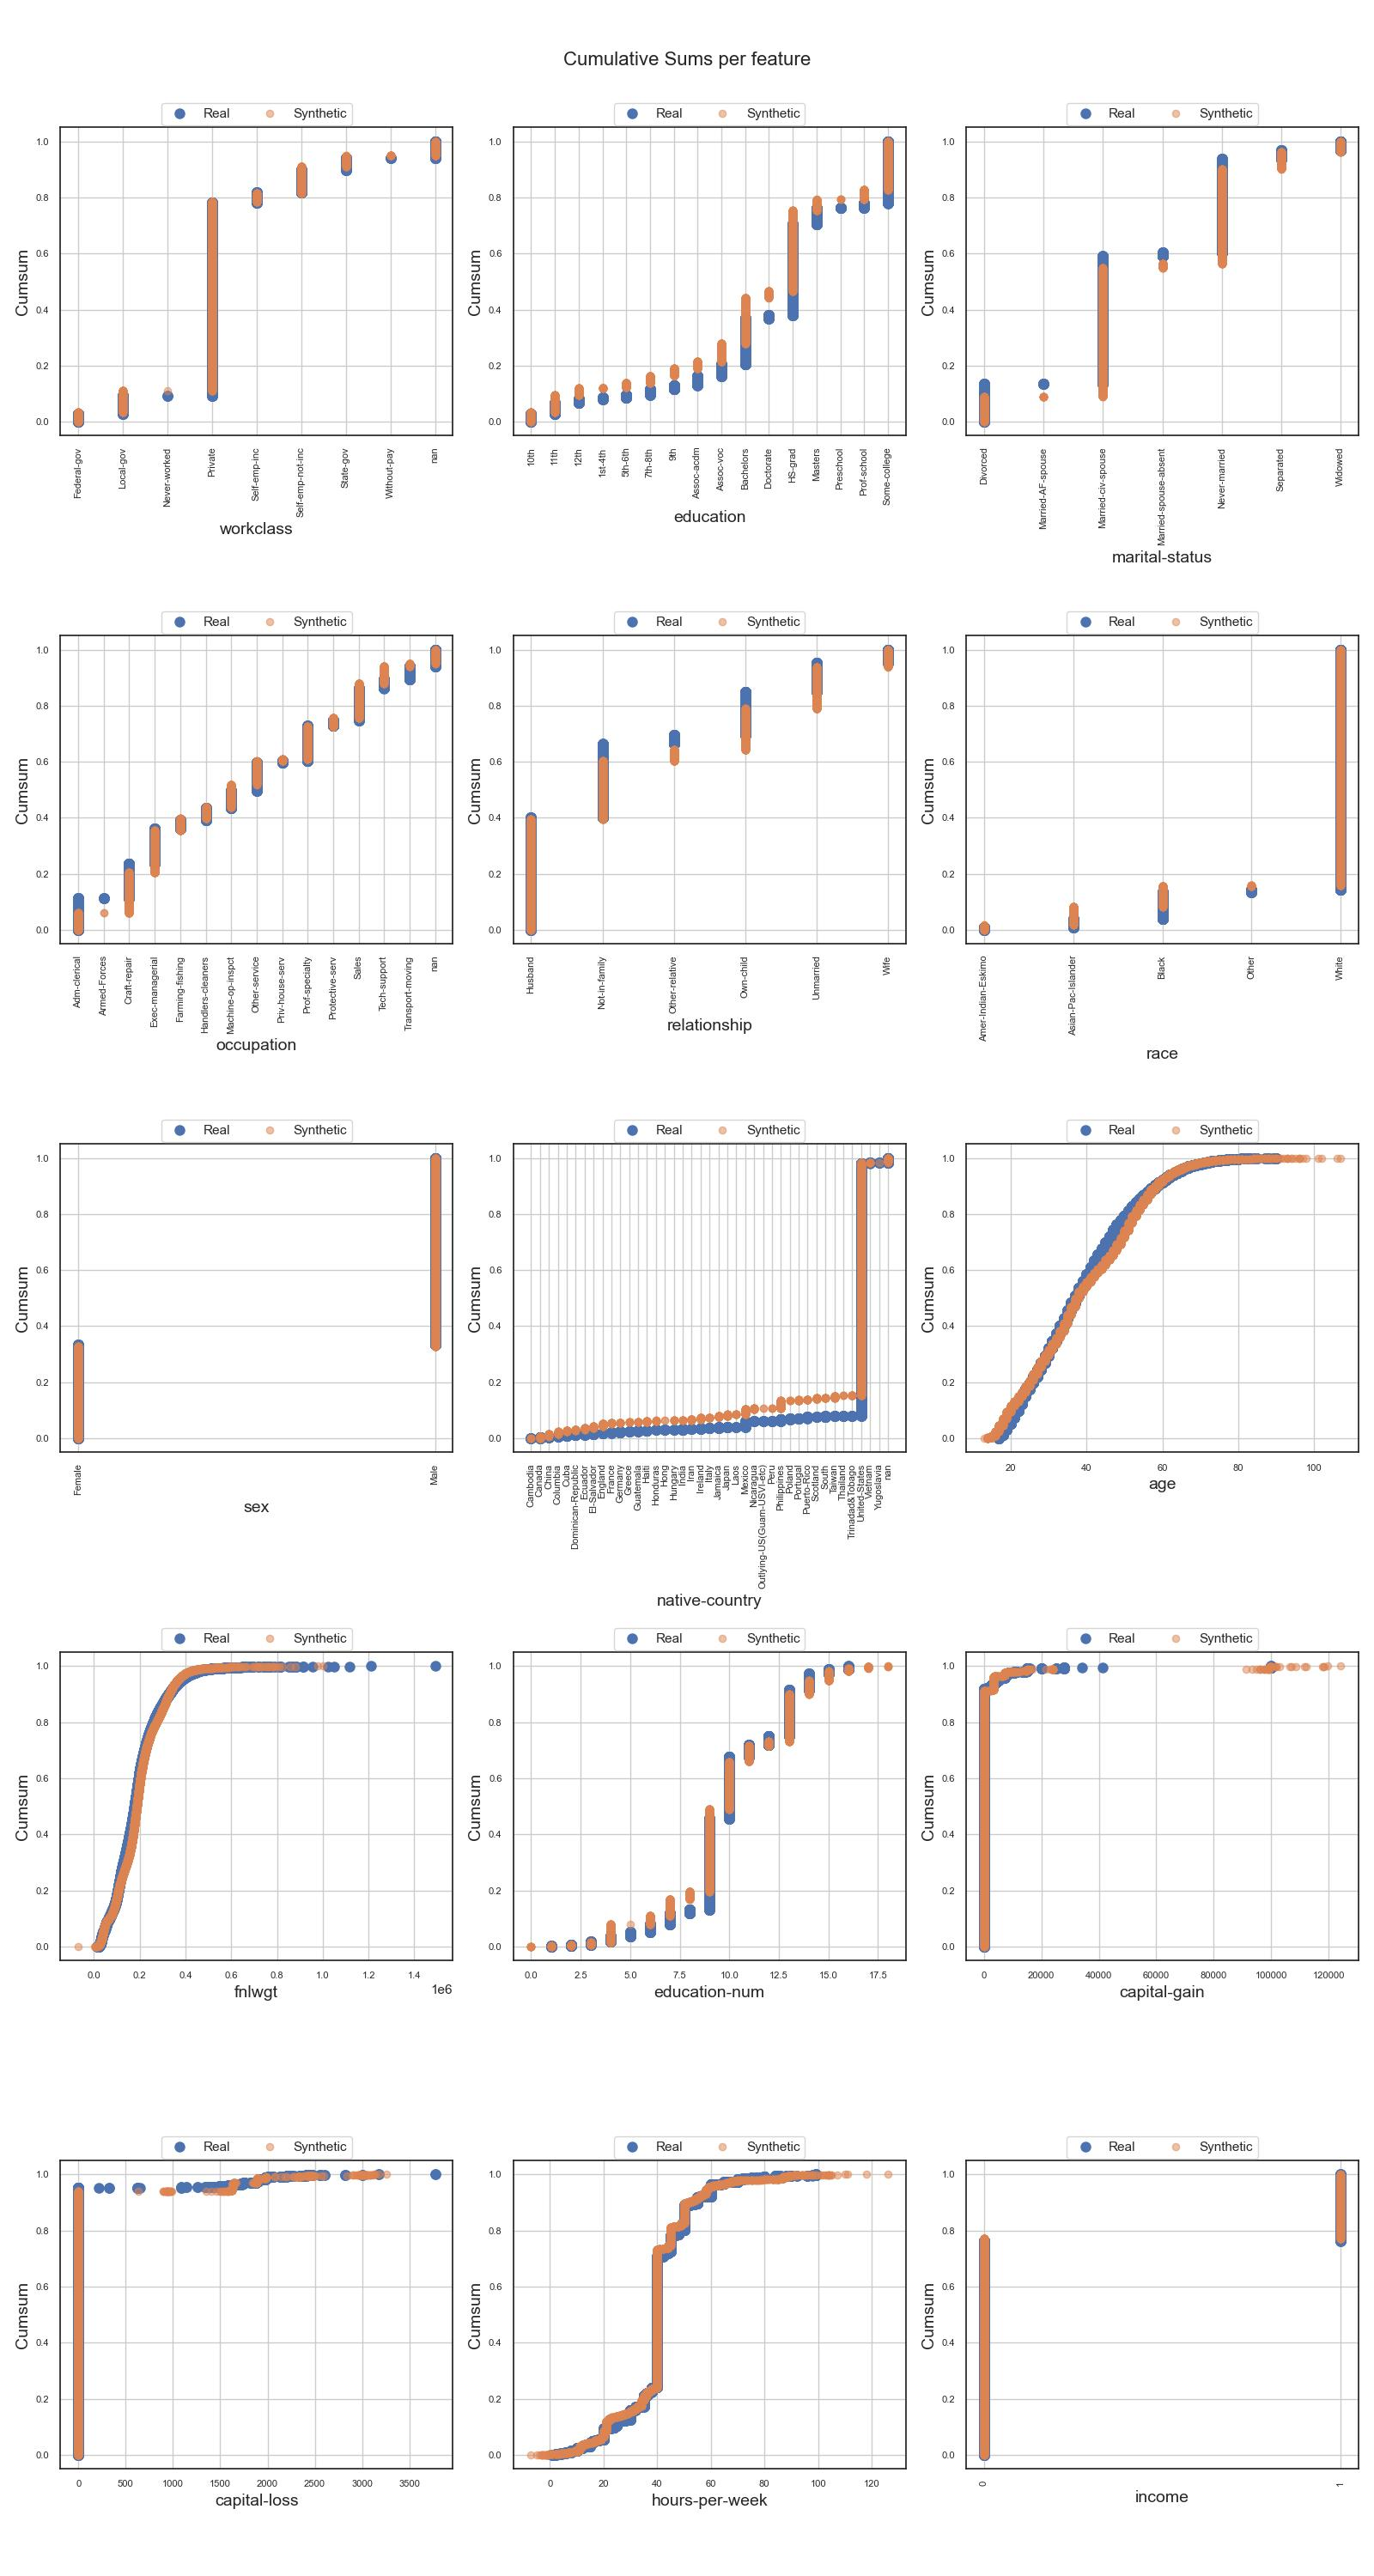
\includegraphics[height=\textheight,width=\linewidth,keepaspectratio]{images/cumsums/ctabgan_simTune.jpg}
			\caption{CTABGAN$^s$}
		\end{subfigure}	
		\hfill
		\begin{subfigure}{0.3\linewidth}
			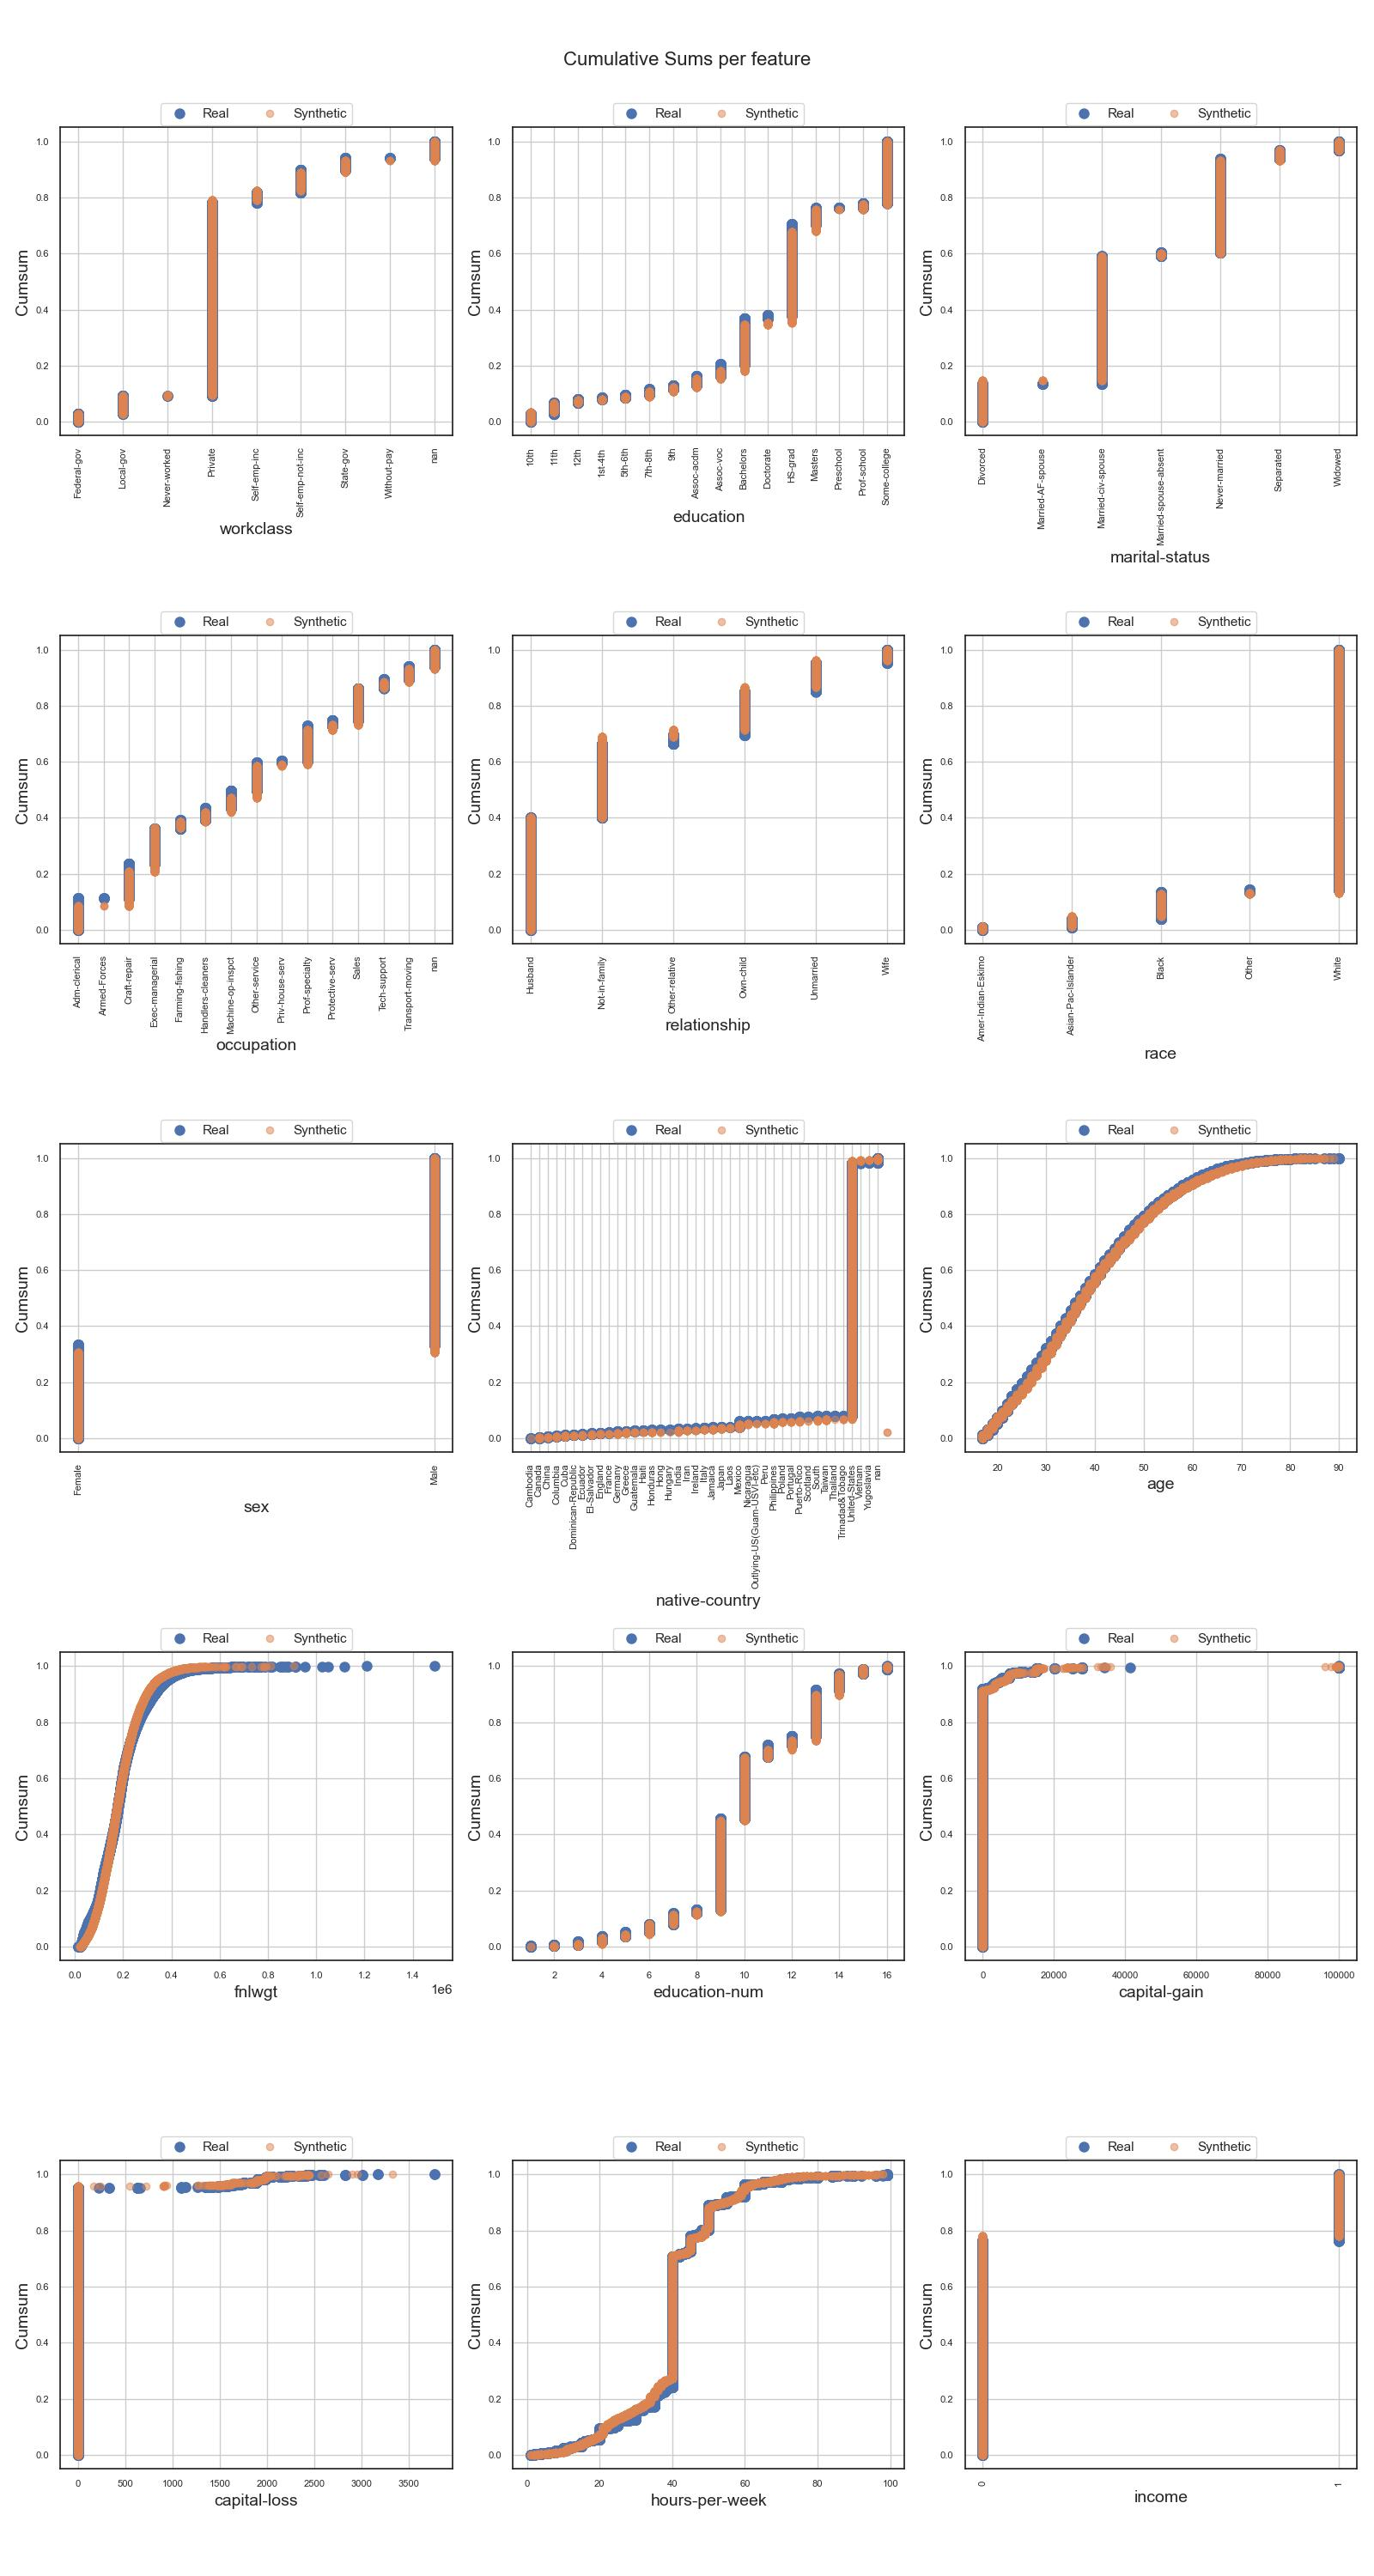
\includegraphics[height=\textheight,width=\linewidth,keepaspectratio]{images/cumsums/ctabgan+.jpg}
			\caption{CTABGAN+$^{ml}$}
		\end{subfigure}
		\hfill
		\caption{Cumulative Distribution plots for CTABGAN$^{ml}$, CTABGAN$^s$ and CTABGAN+$^{ml}$}
		\label{fig_a:cumsum_1}
	\end{figure}
\end{landscape}
%----------
\newpage
\begin{landscape}
	\begin{figure}[h]
		\centering
		\hfill
		\begin{subfigure}{0.3\linewidth}
			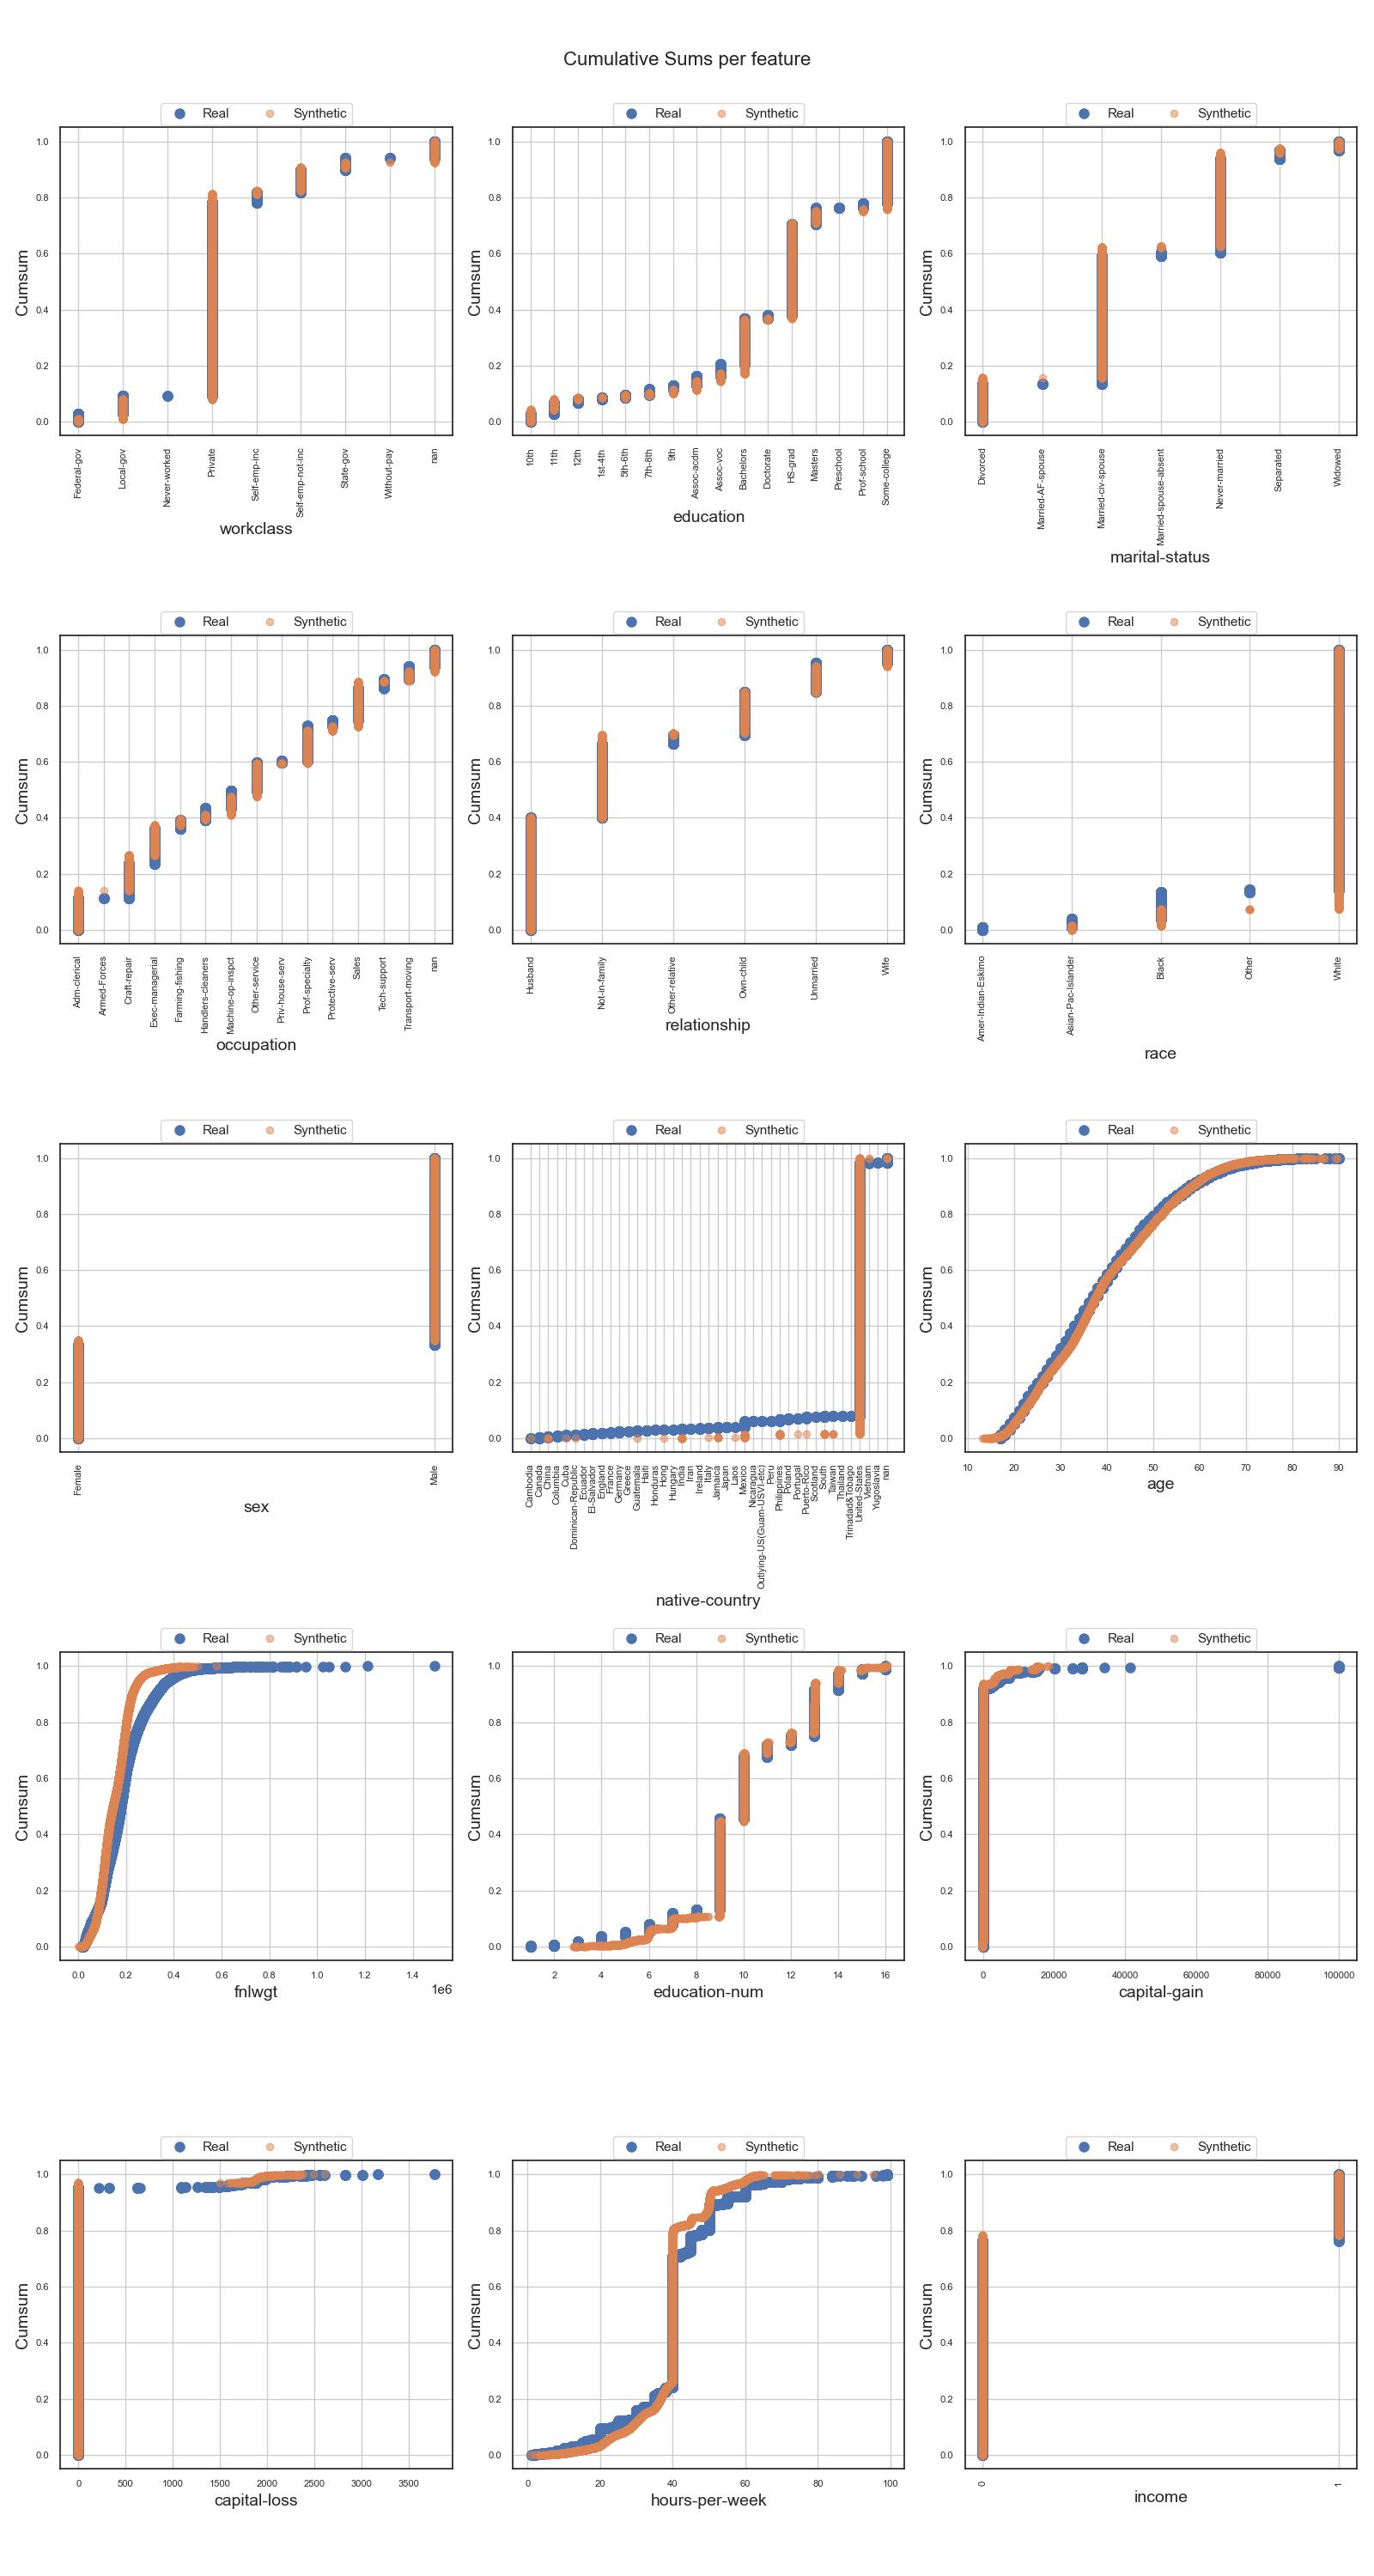
\includegraphics[height=\textheight,width=\linewidth,keepaspectratio]{images/cumsums/tvae.jpg}
			\caption{TVAE$^{ml}$}
		\end{subfigure}		
		\hfill
		\begin{subfigure}{0.3\linewidth}
			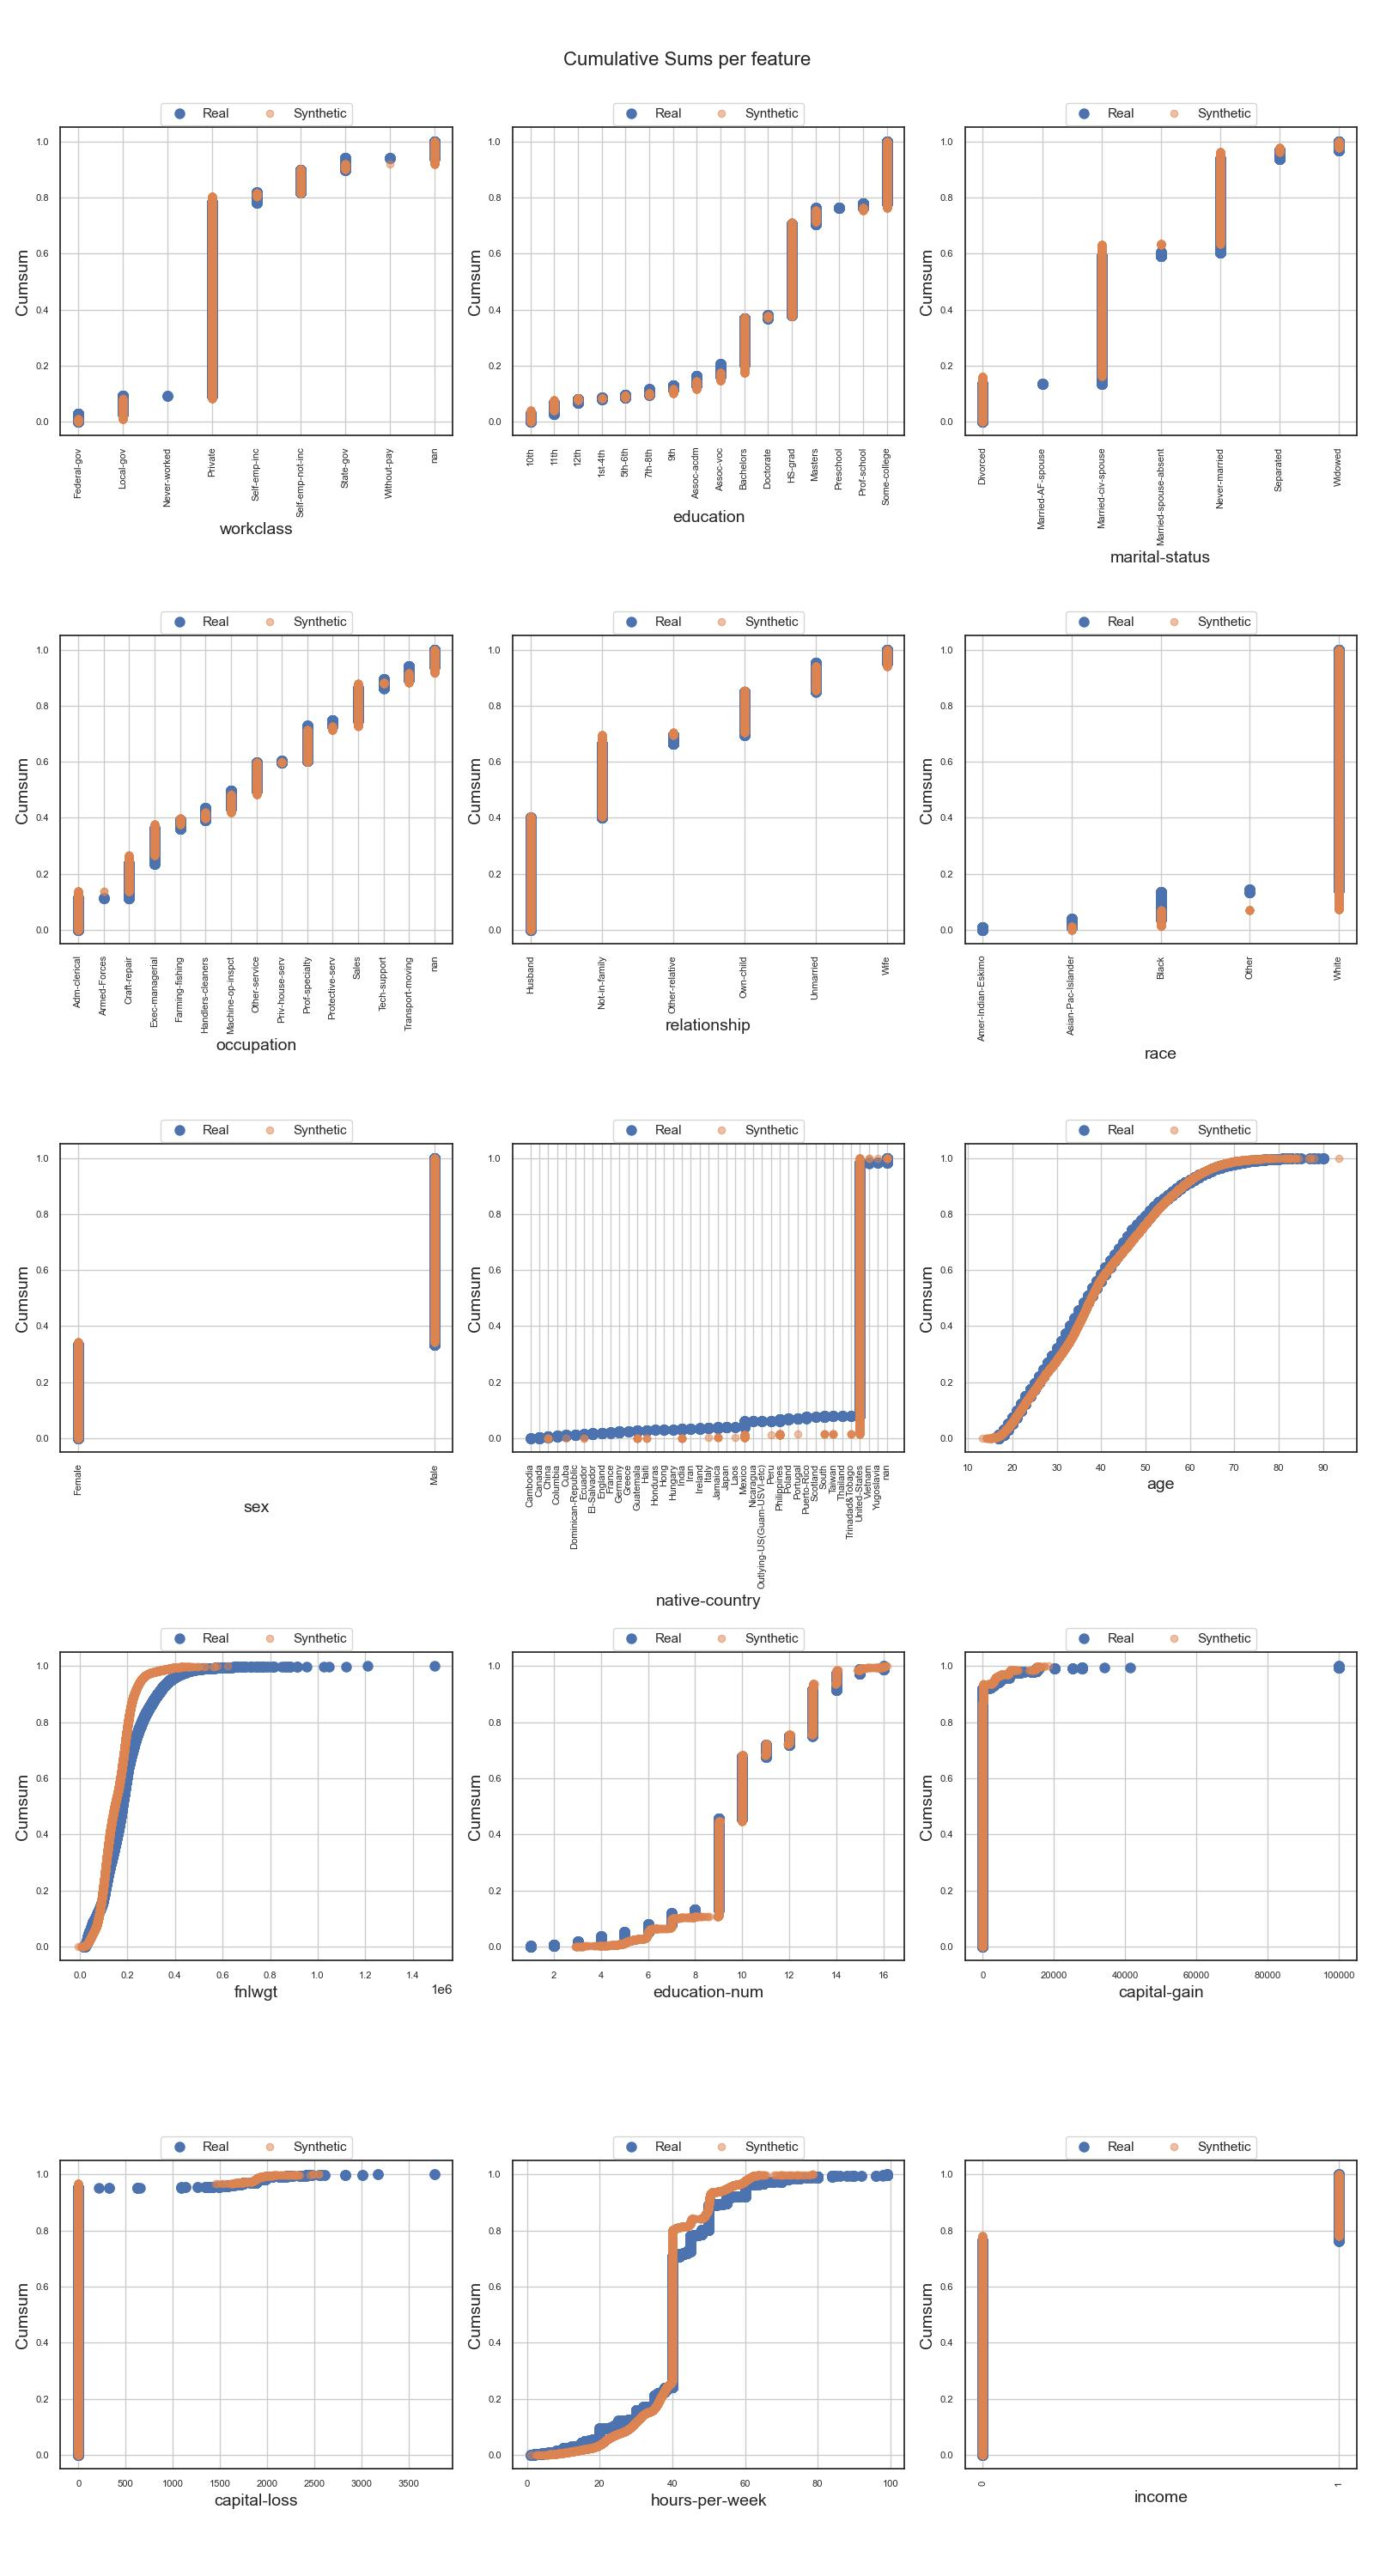
\includegraphics[height=\textheight,width=\linewidth,keepaspectratio]{images/cumsums/tvae_simTune.jpg}
			\caption{TVAE$^s$}
		\end{subfigure}
		\hfill
		\begin{subfigure}{0.3\linewidth}
			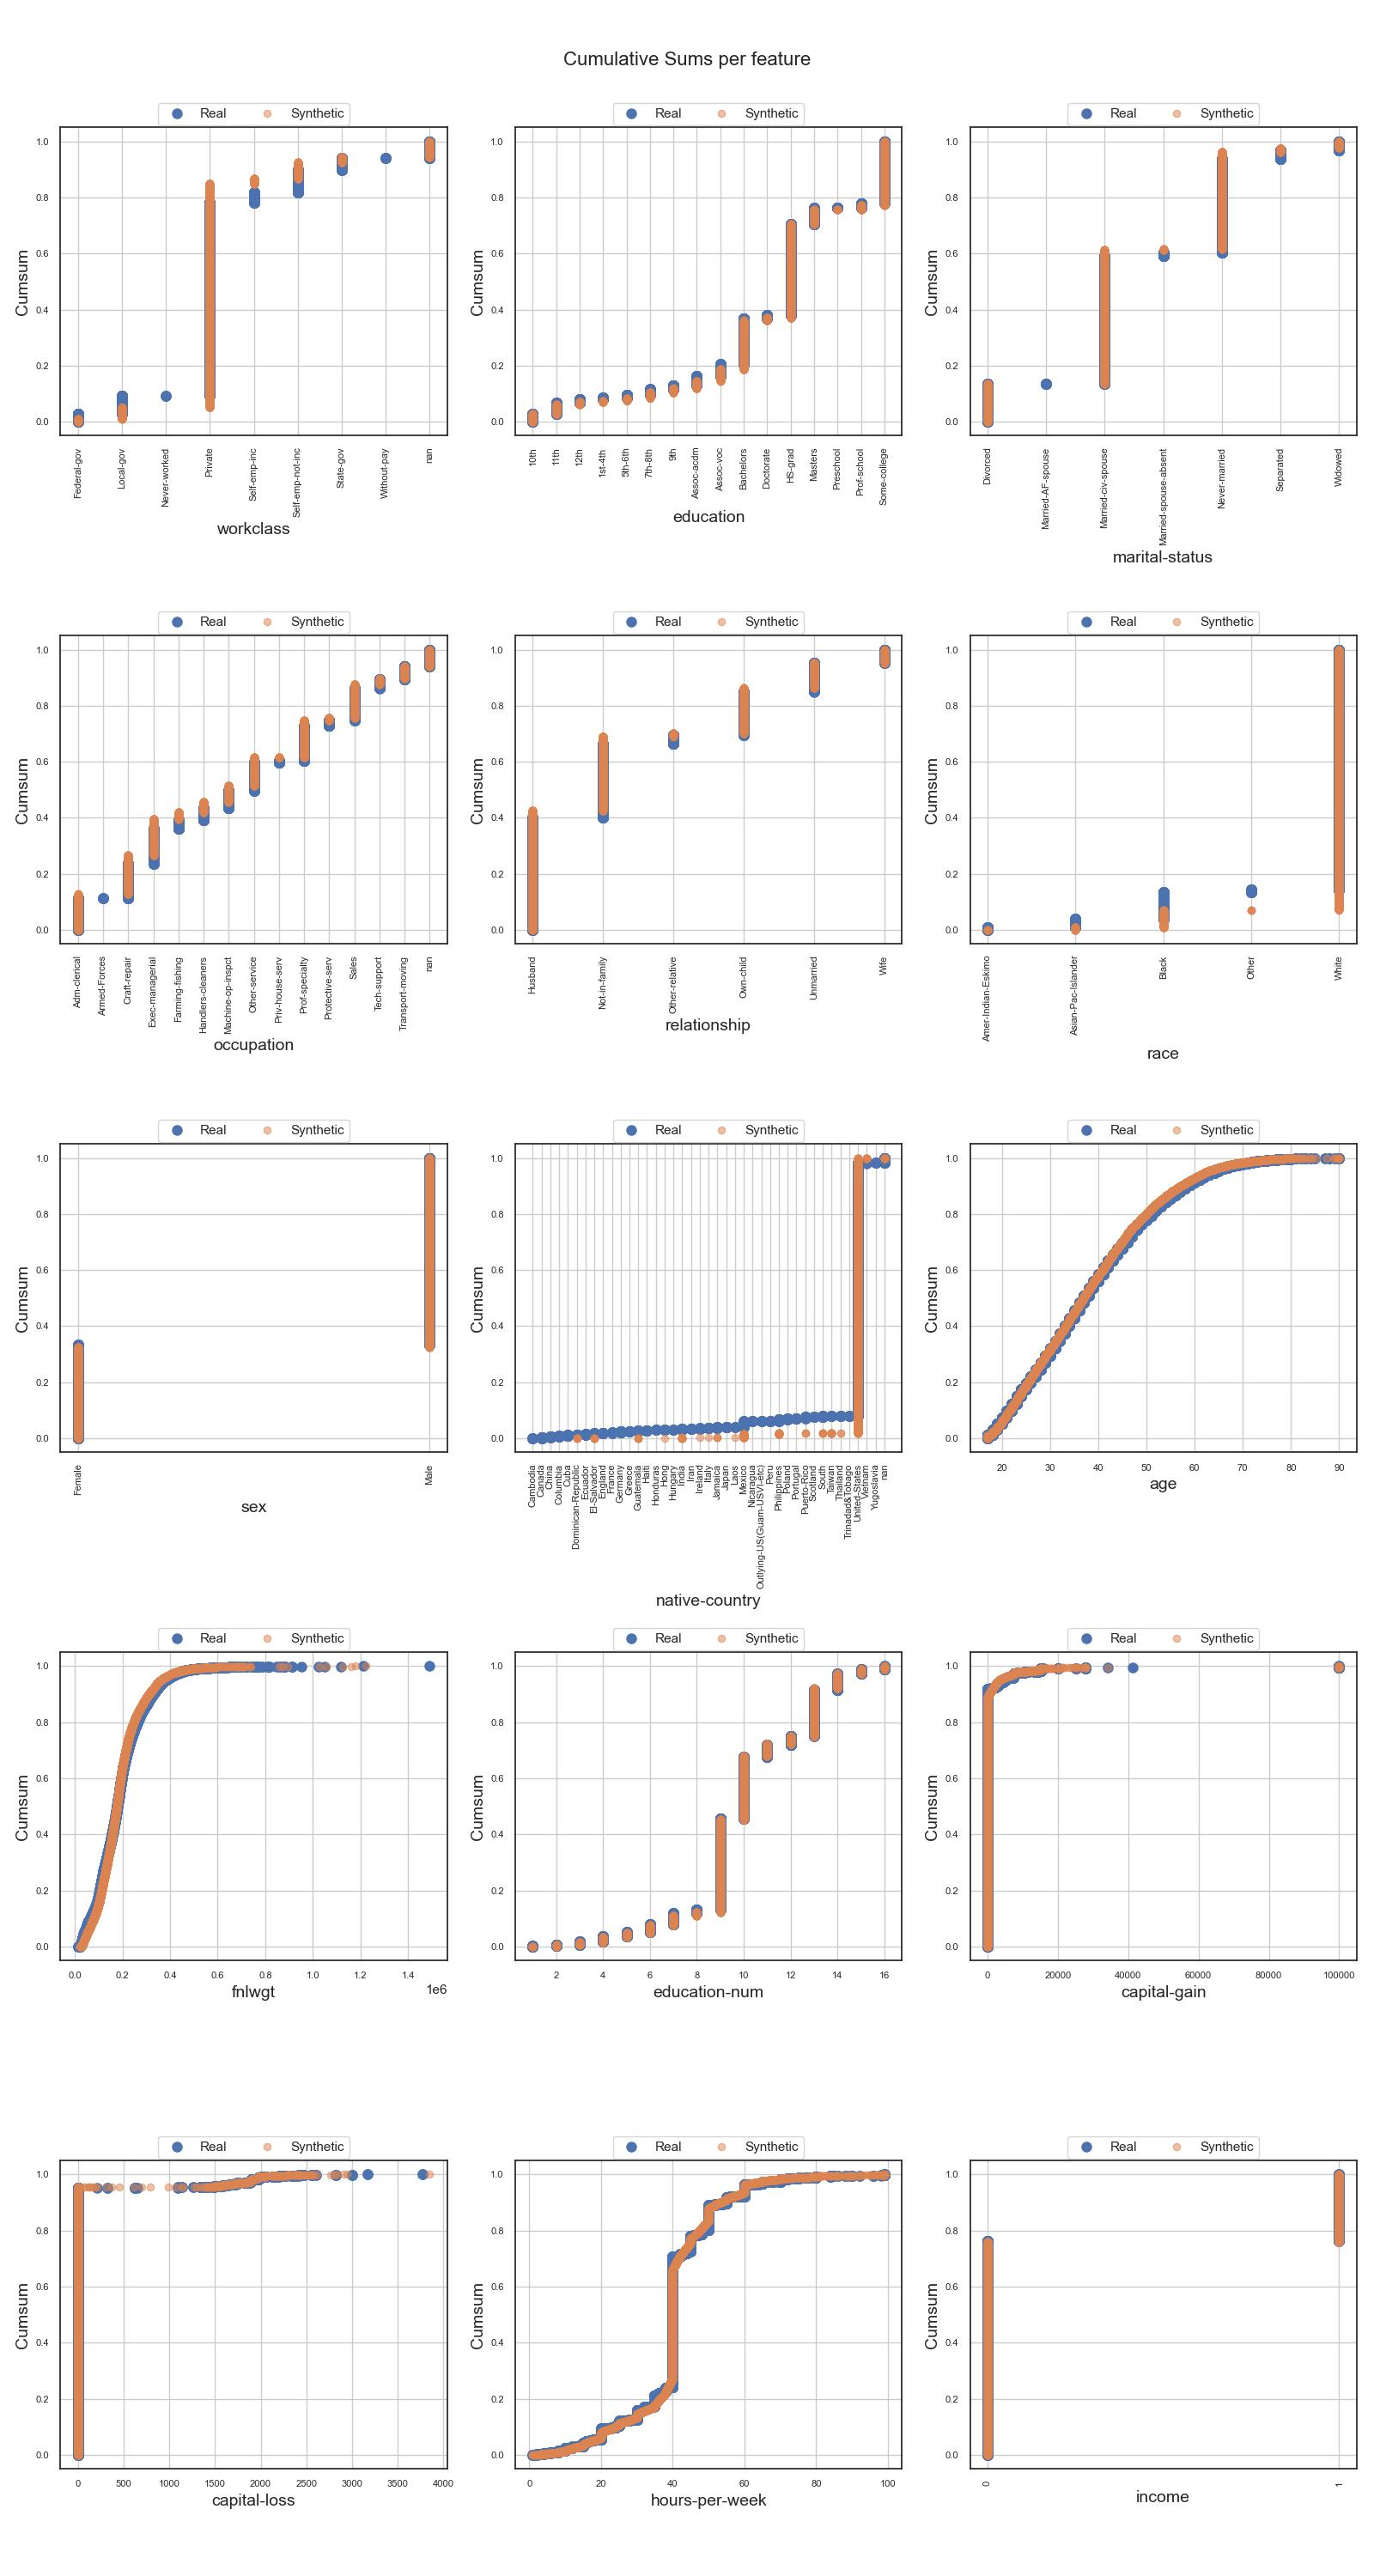
\includegraphics[height=\textheight,width=\linewidth,keepaspectratio]{images/cumsums/smote.jpg}
			\caption{SMOTE}
		\end{subfigure}
		\caption{Cumulative Distribution plots for TVAE$^{ml}$, TVAE$^s$ and SMOTE}
		\label{fig_a:cumsum_2}
	\end{figure}
\end{landscape}
%----------
\newpage
\begin{landscape}
	\begin{figure}[h]
		\centering
		\hfill
		\begin{subfigure}{0.3\linewidth}
			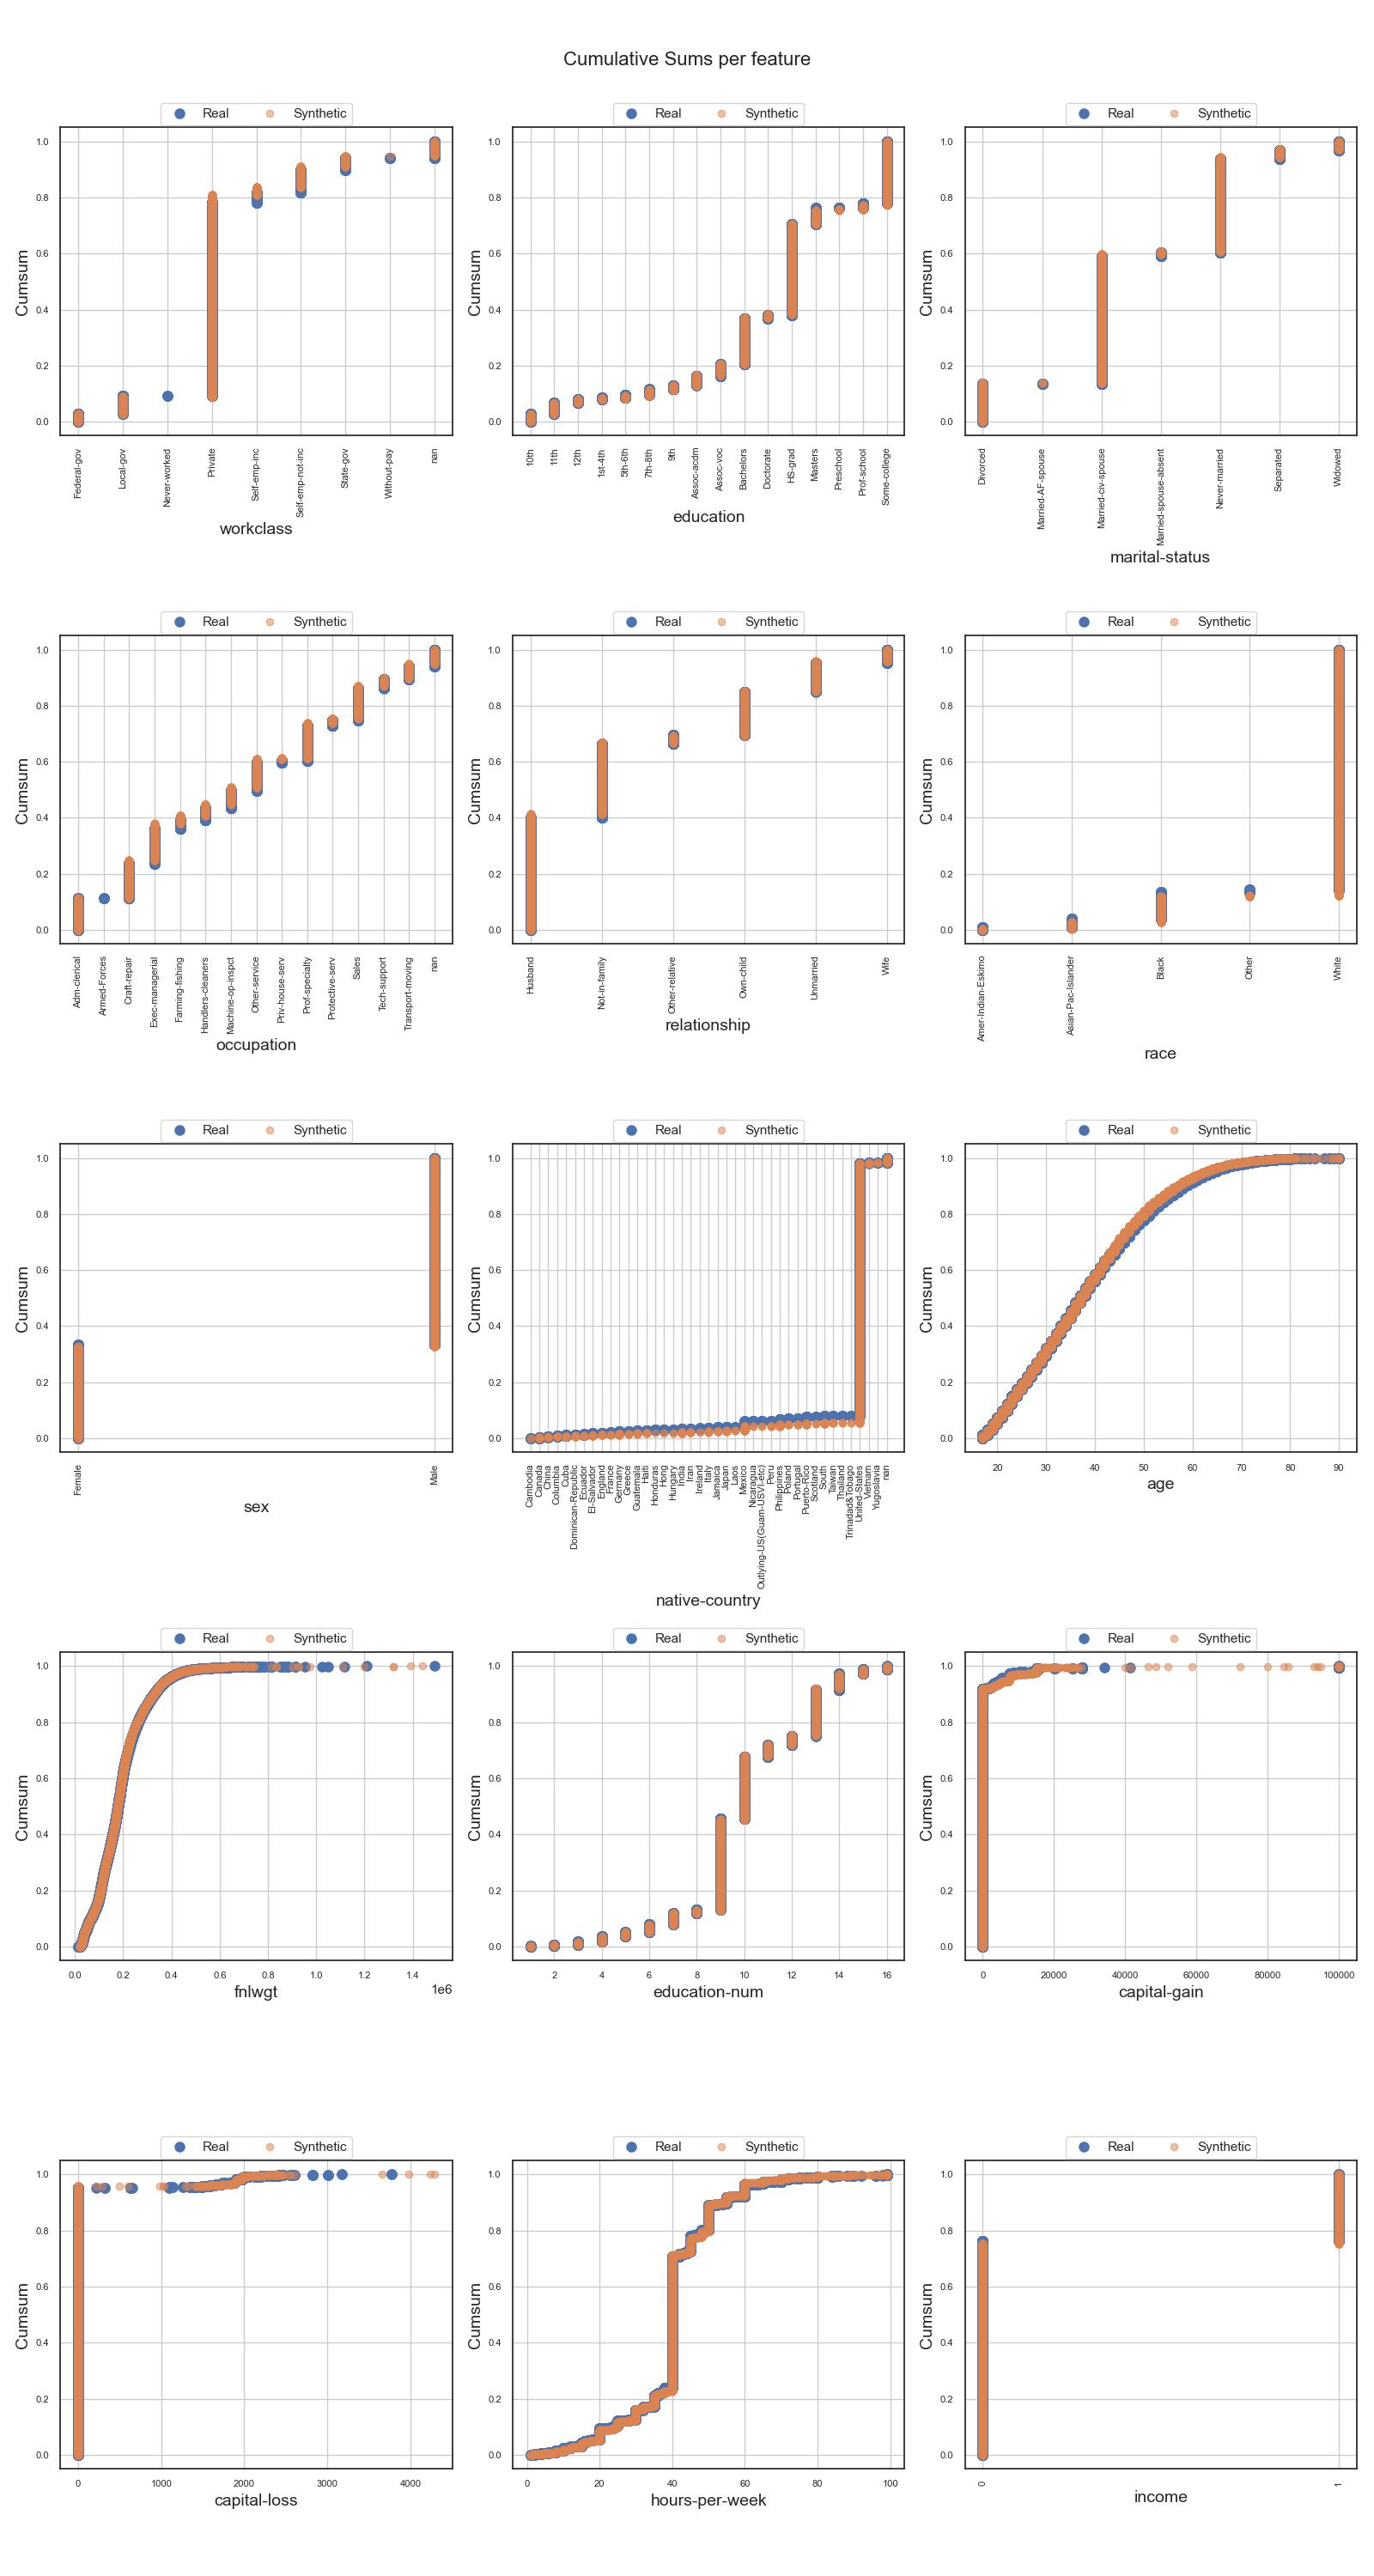
\includegraphics[height=\textheight,width=\linewidth,keepaspectratio]{images/cumsums/tab-ddpm.jpg}
			\caption{TabDDPM$^{ml}_q$}
		\end{subfigure}
		\hfill
		\begin{subfigure}{0.3\linewidth}
			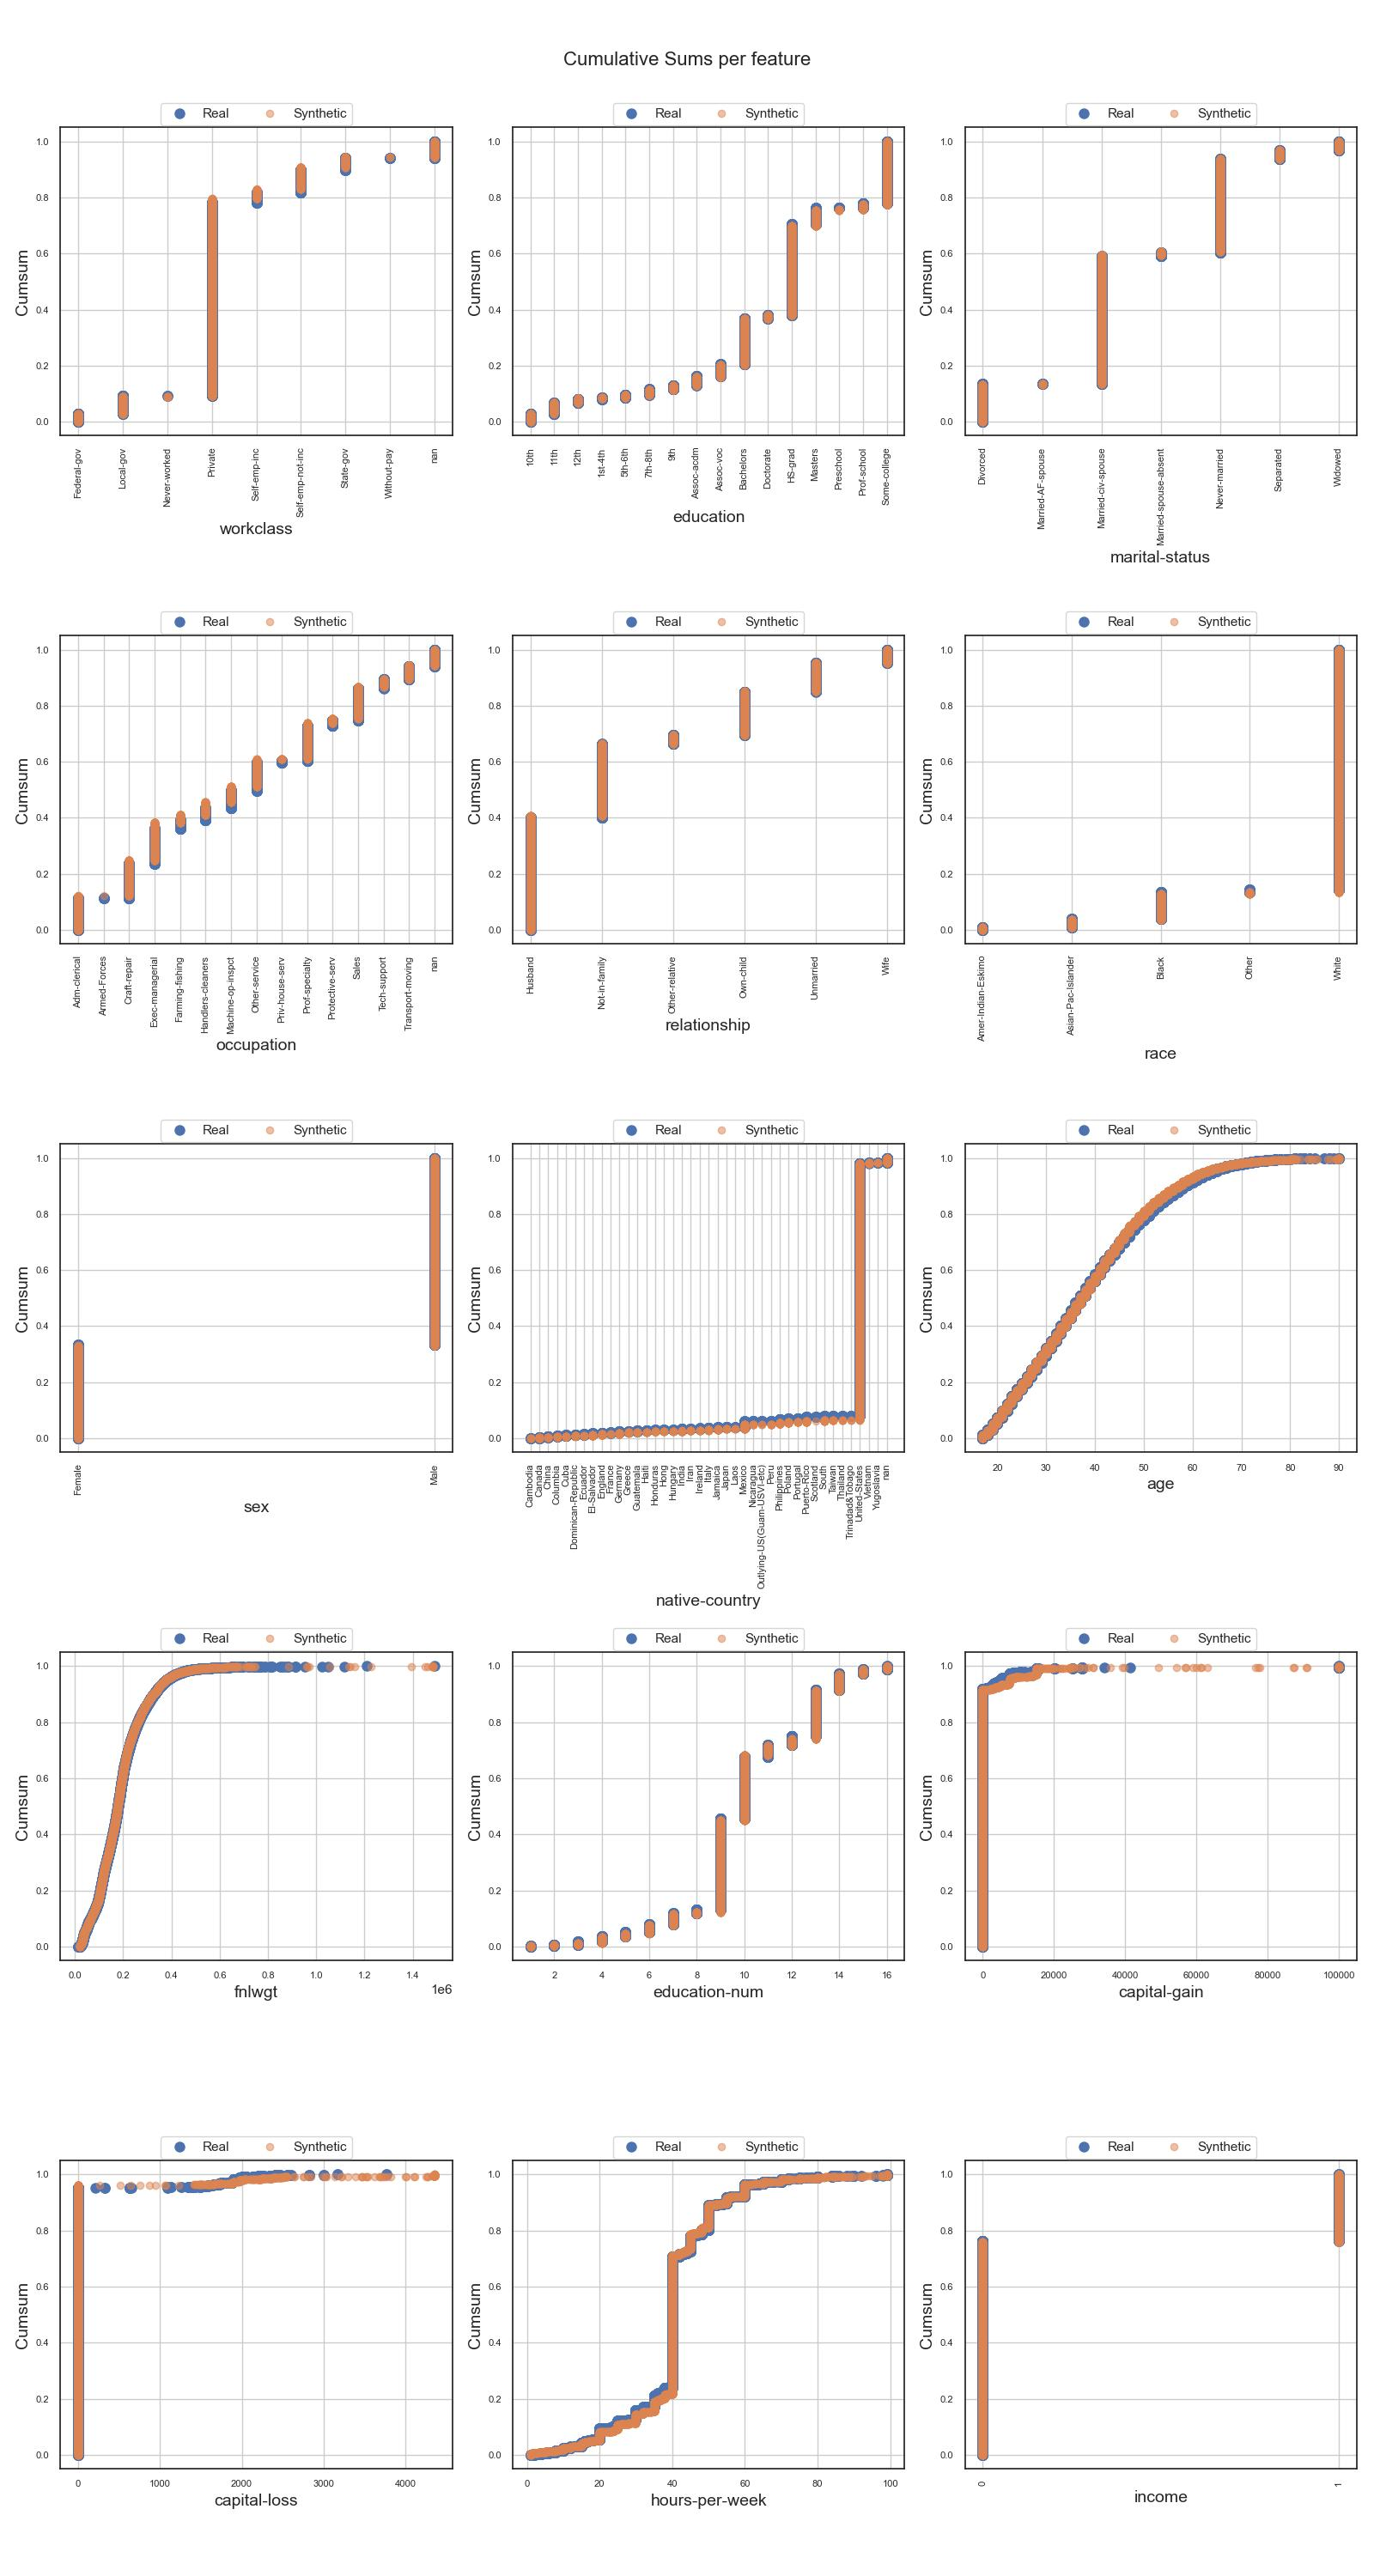
\includegraphics[height=\textheight,width=\linewidth,keepaspectratio]{images/cumsums/tab-ddpm-simTune.jpg}
			\caption{TabDDPM$^{s}_q$}
		\end{subfigure}
		\hfill
		\begin{subfigure}{0.3\linewidth}
			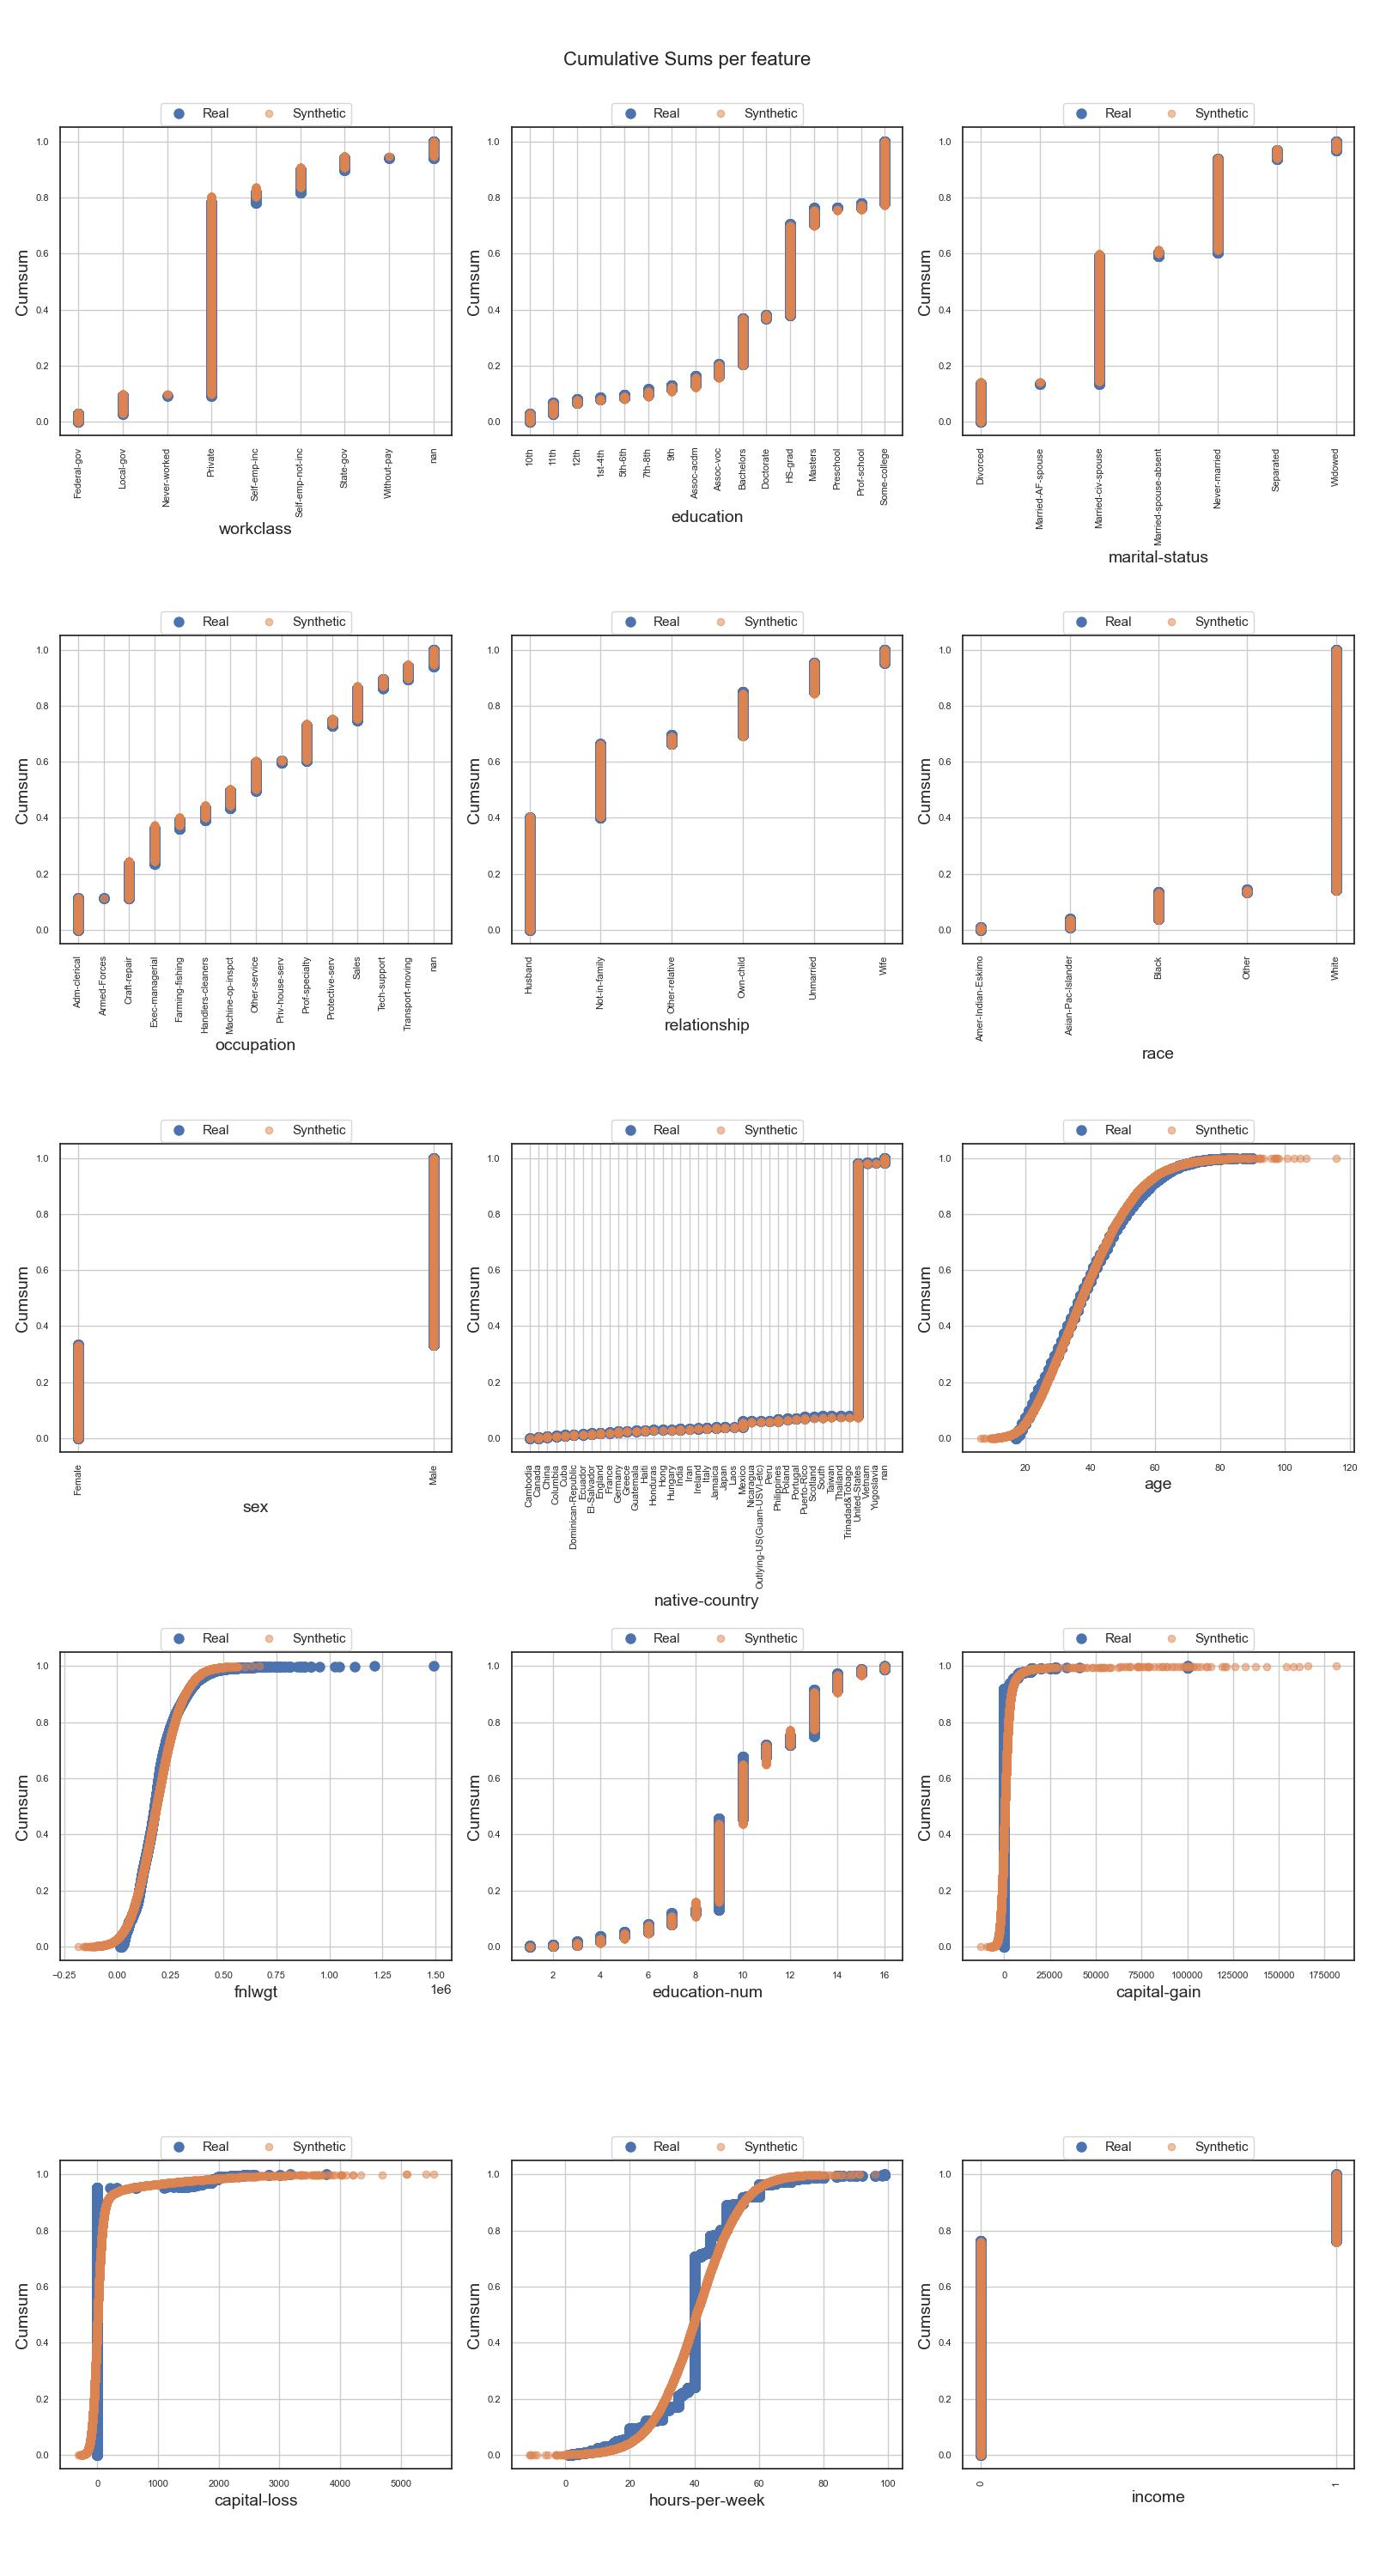
\includegraphics[height=\textheight,width=\linewidth,keepaspectratio]{images/cumsums/tab-ddpm-simTune-minmax.jpg}
			\caption{TabDDPM$^{s}_m$}
		\end{subfigure}
		\hfill
		\caption{Cumulative Distribution plots for TabDDPM variations}
		\label{fig_a:cumsum_3}
	\end{figure}
\end{landscape}
%----------
\newpage
\begin{landscape}
	\begin{figure}[h]
		\centering
		\hfill
		\begin{subfigure}{0.3\linewidth}
			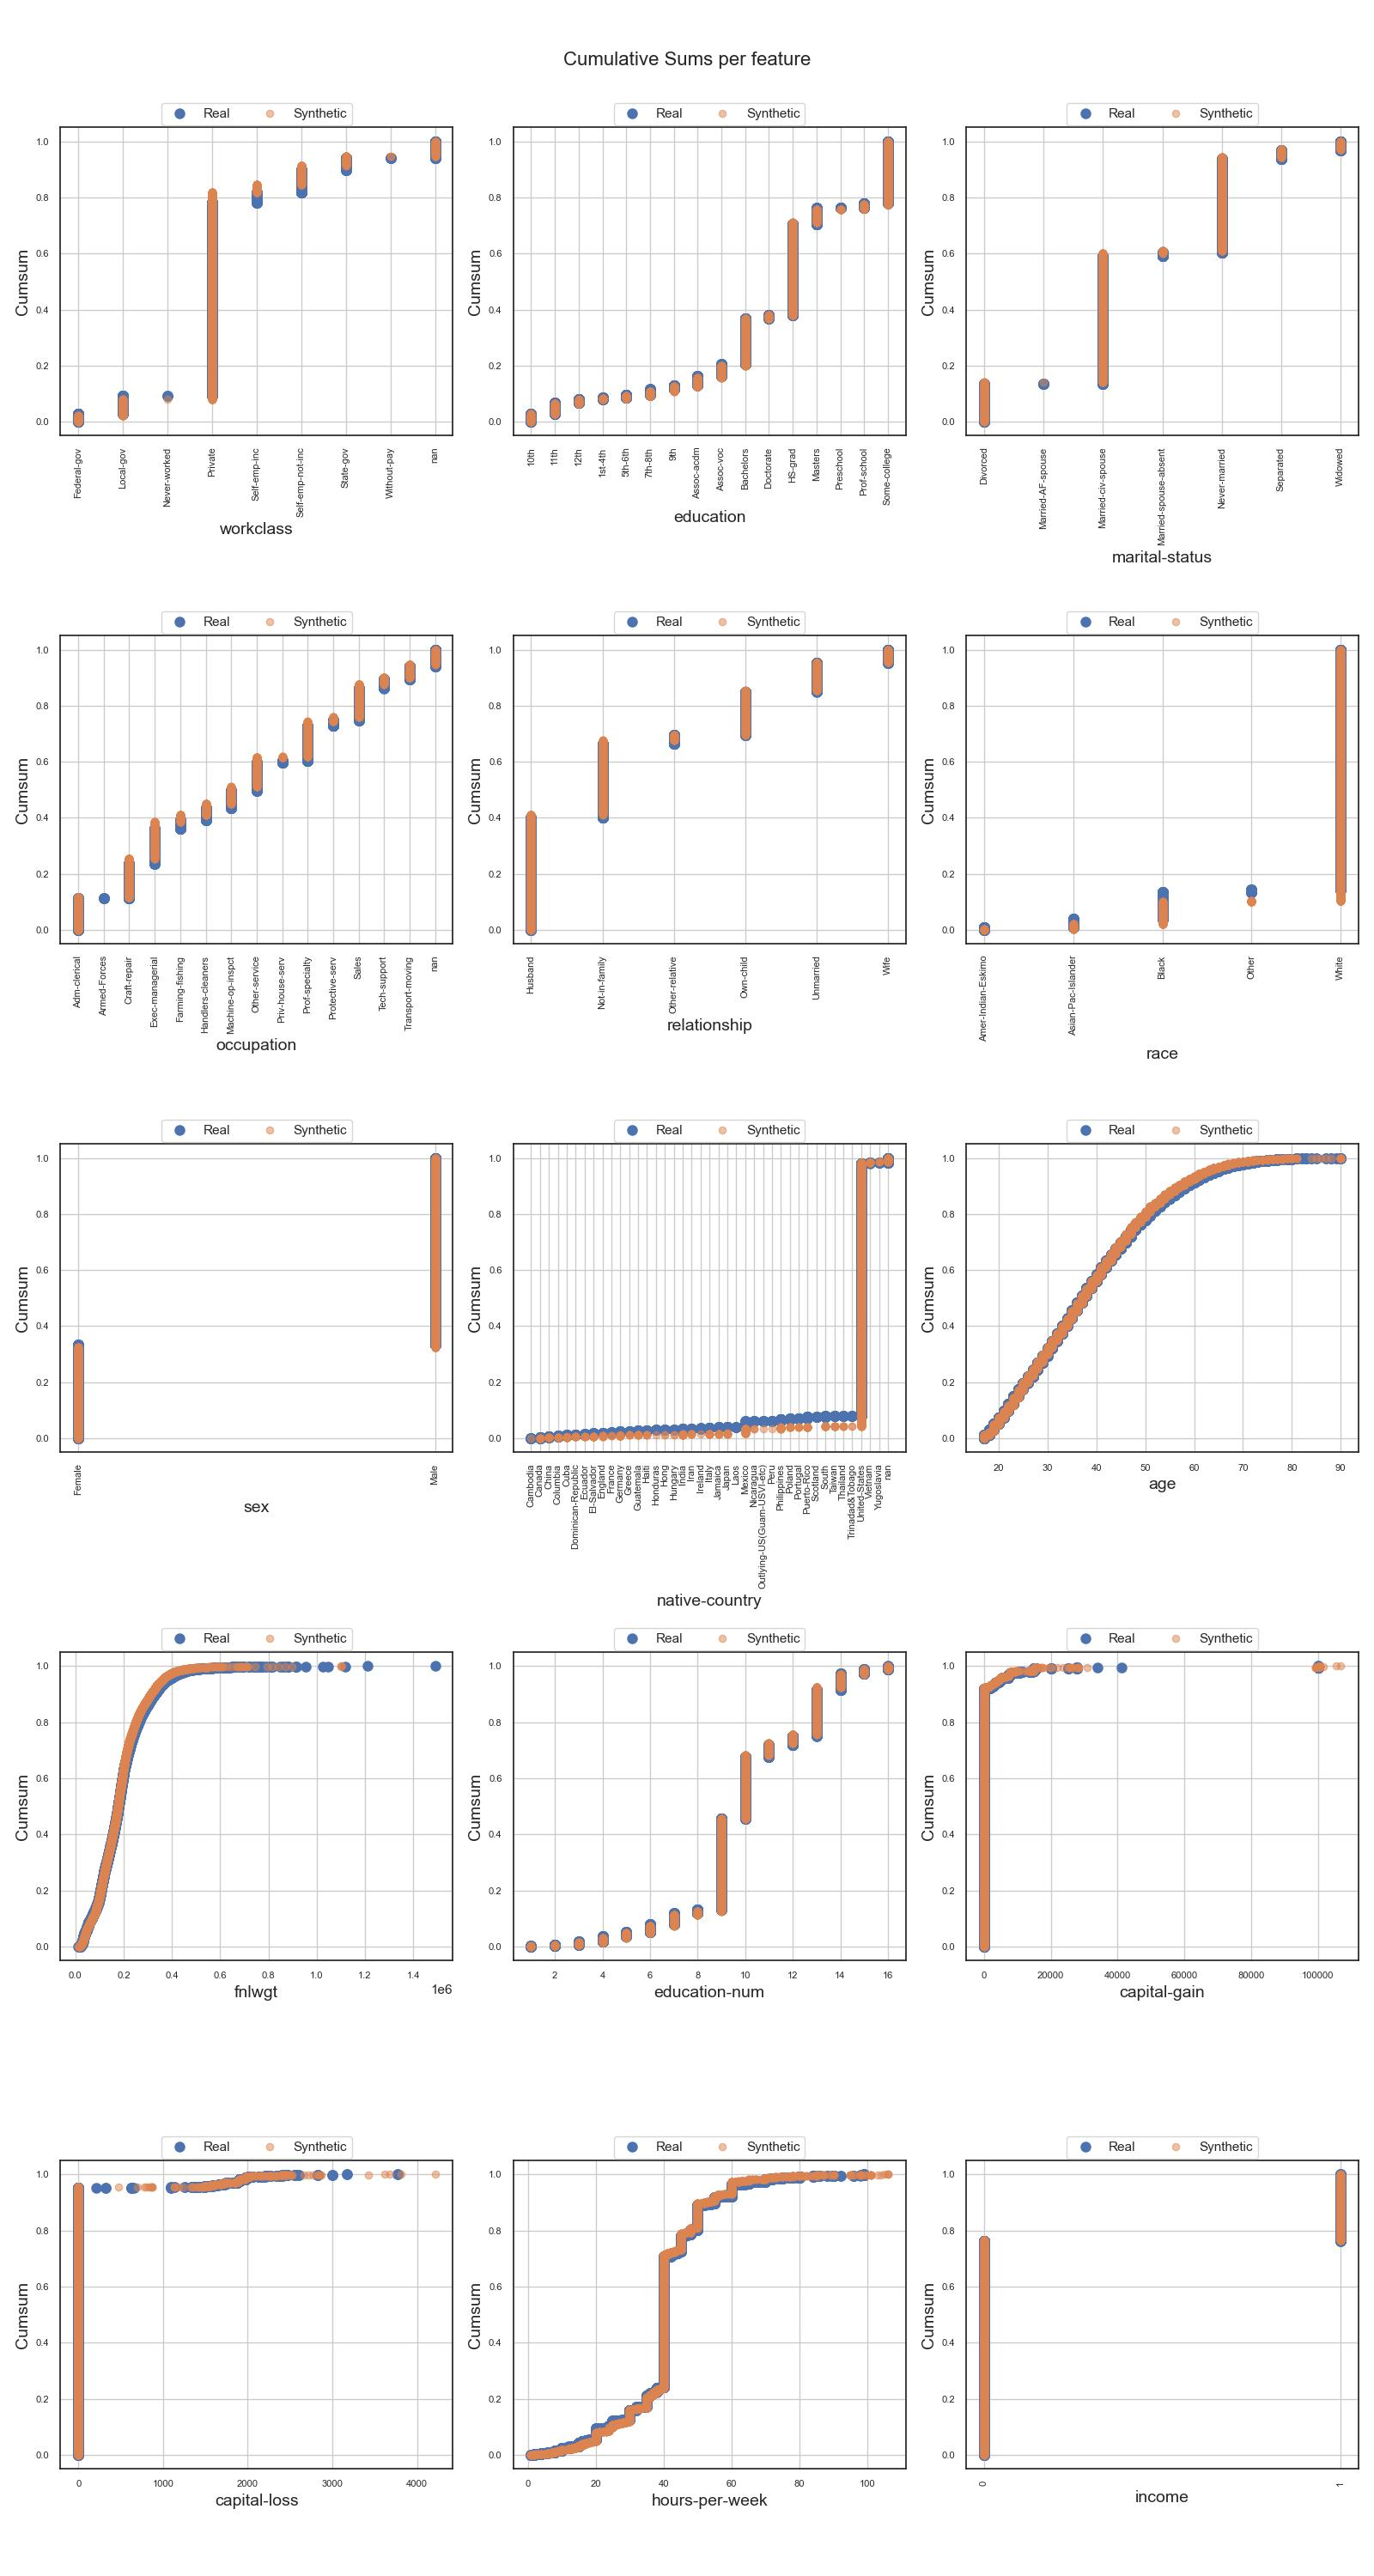
\includegraphics[height=\textheight,width=\linewidth,keepaspectratio]{images/cumsums/tab-ddpm-bgm.jpg}
			\caption{TabDDPM-BGM$^{ml}_q$}
		\end{subfigure}
		\hfill
		\begin{subfigure}{0.3\linewidth}
			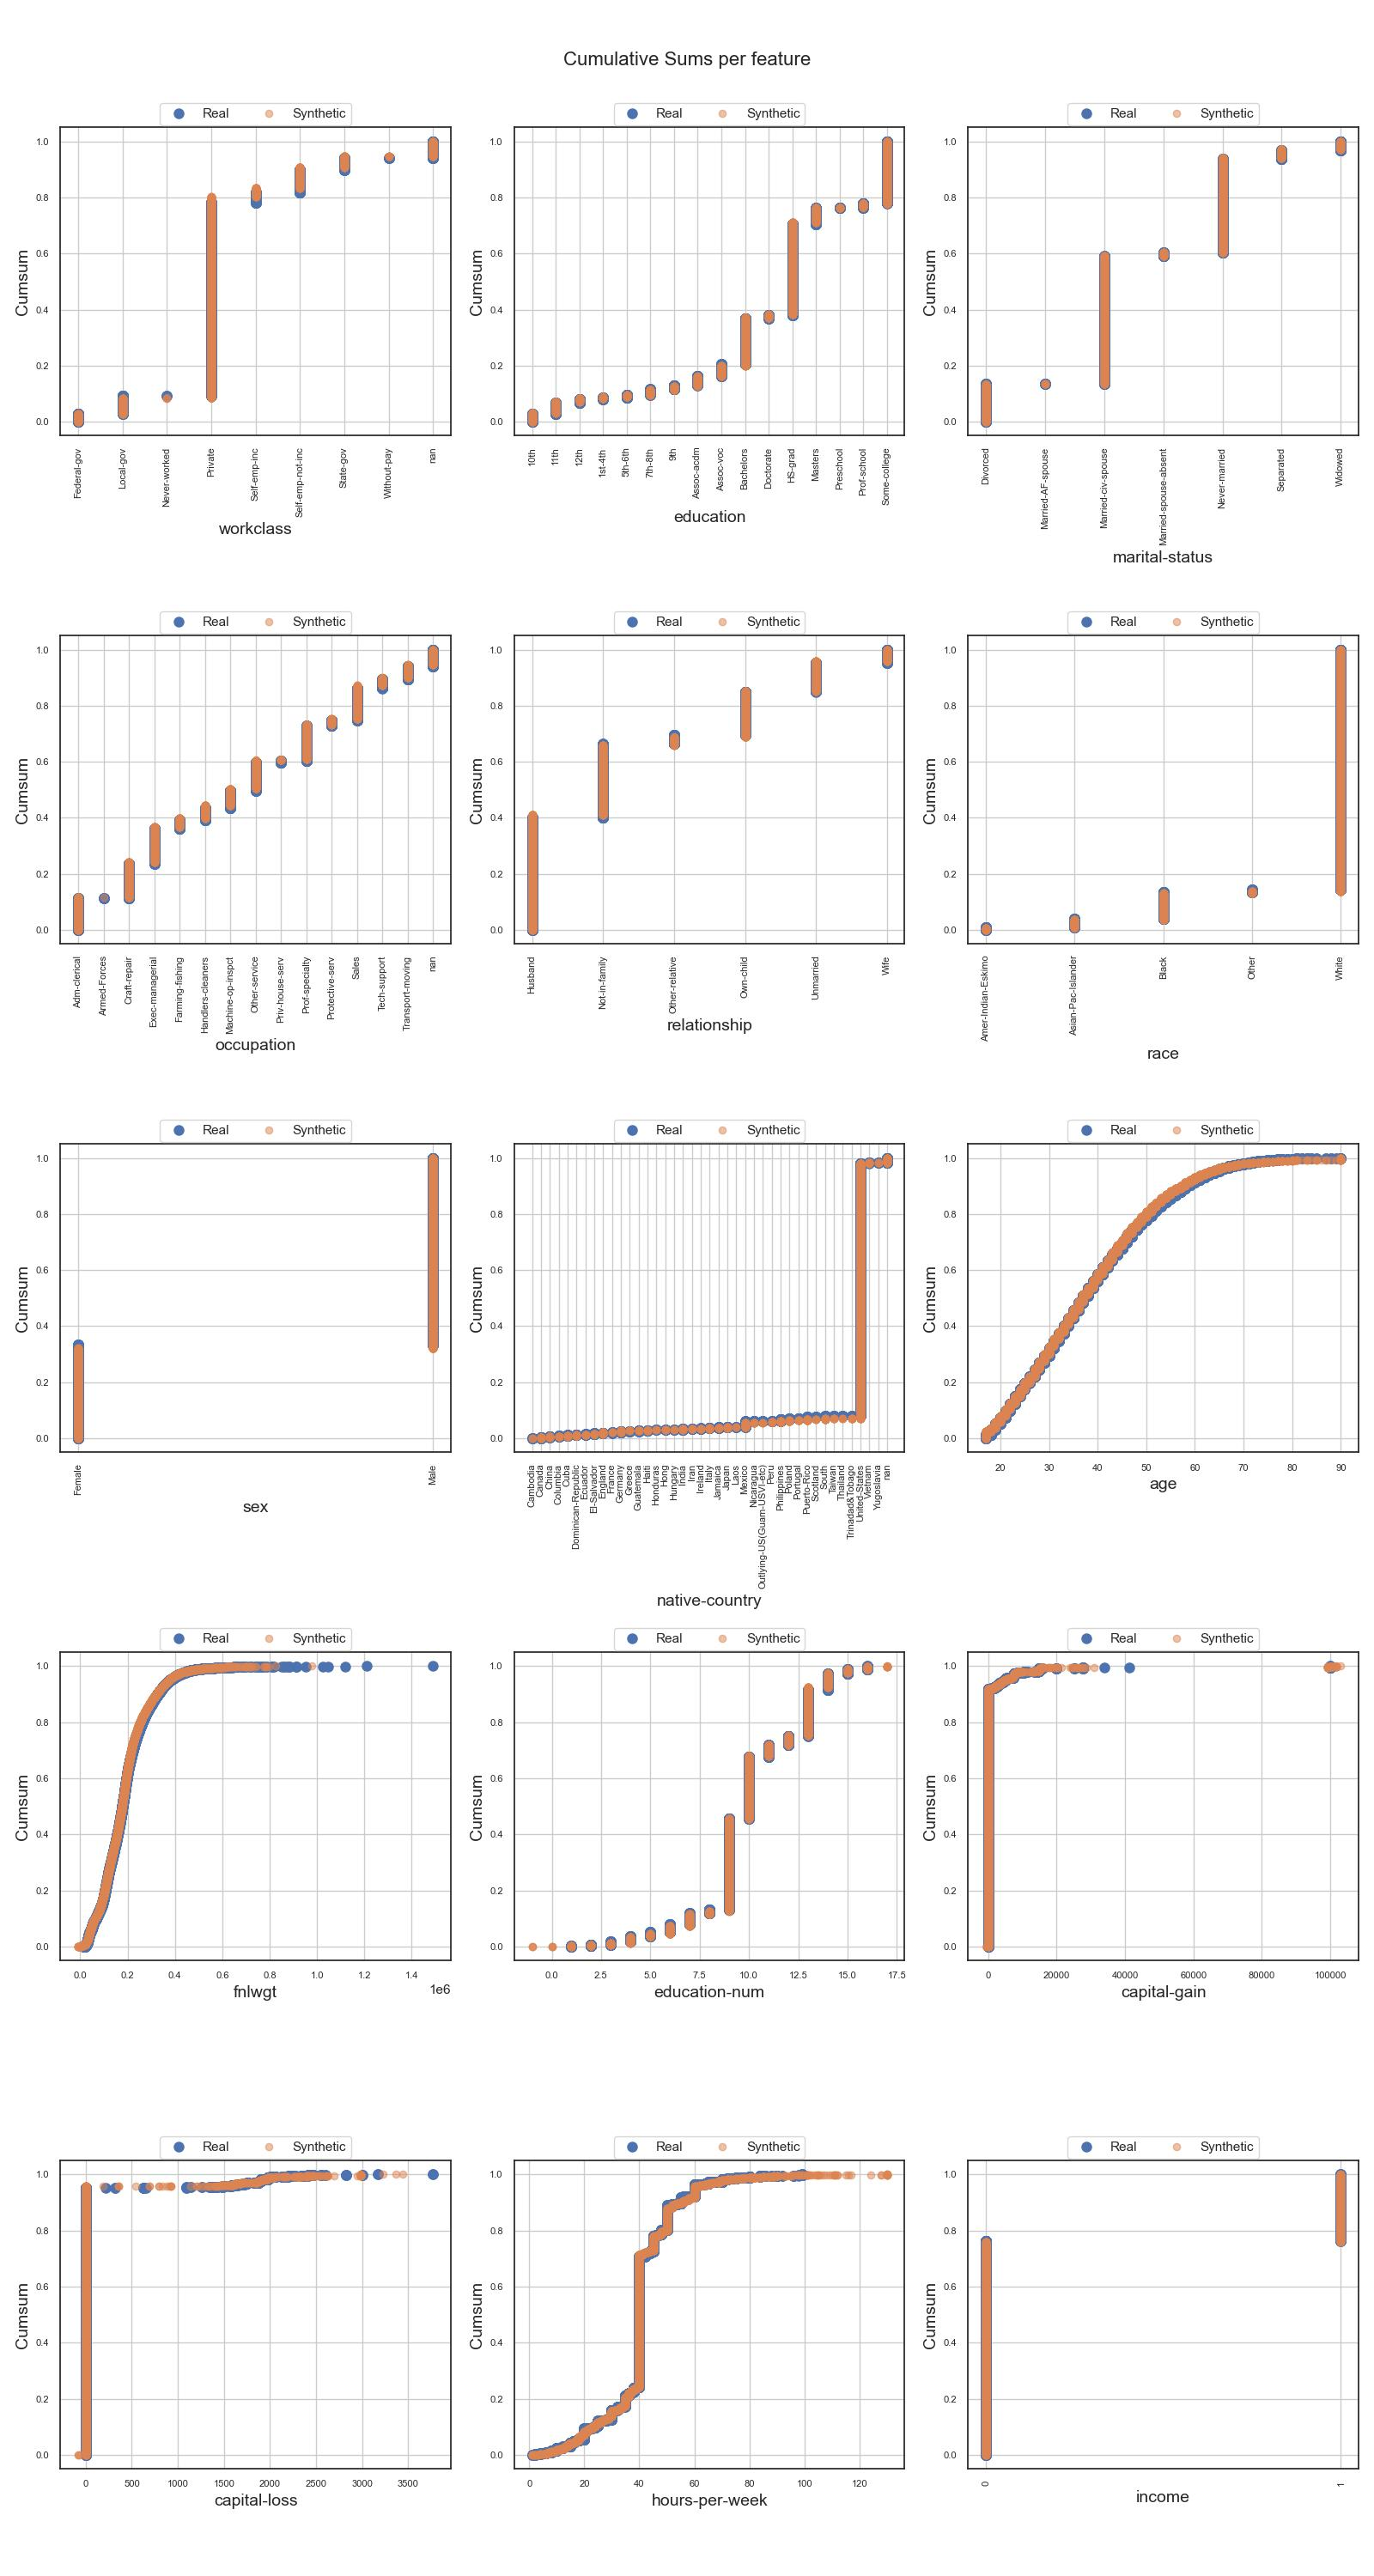
\includegraphics[height=\textheight,width=\linewidth,keepaspectratio]{images/cumsums/tab-ddpm-bgm-simTune.jpg}
			\caption{TabDDPM-BGM$^{s}_q$}
		\end{subfigure}
		\hfill
		\begin{subfigure}{0.3\linewidth}
			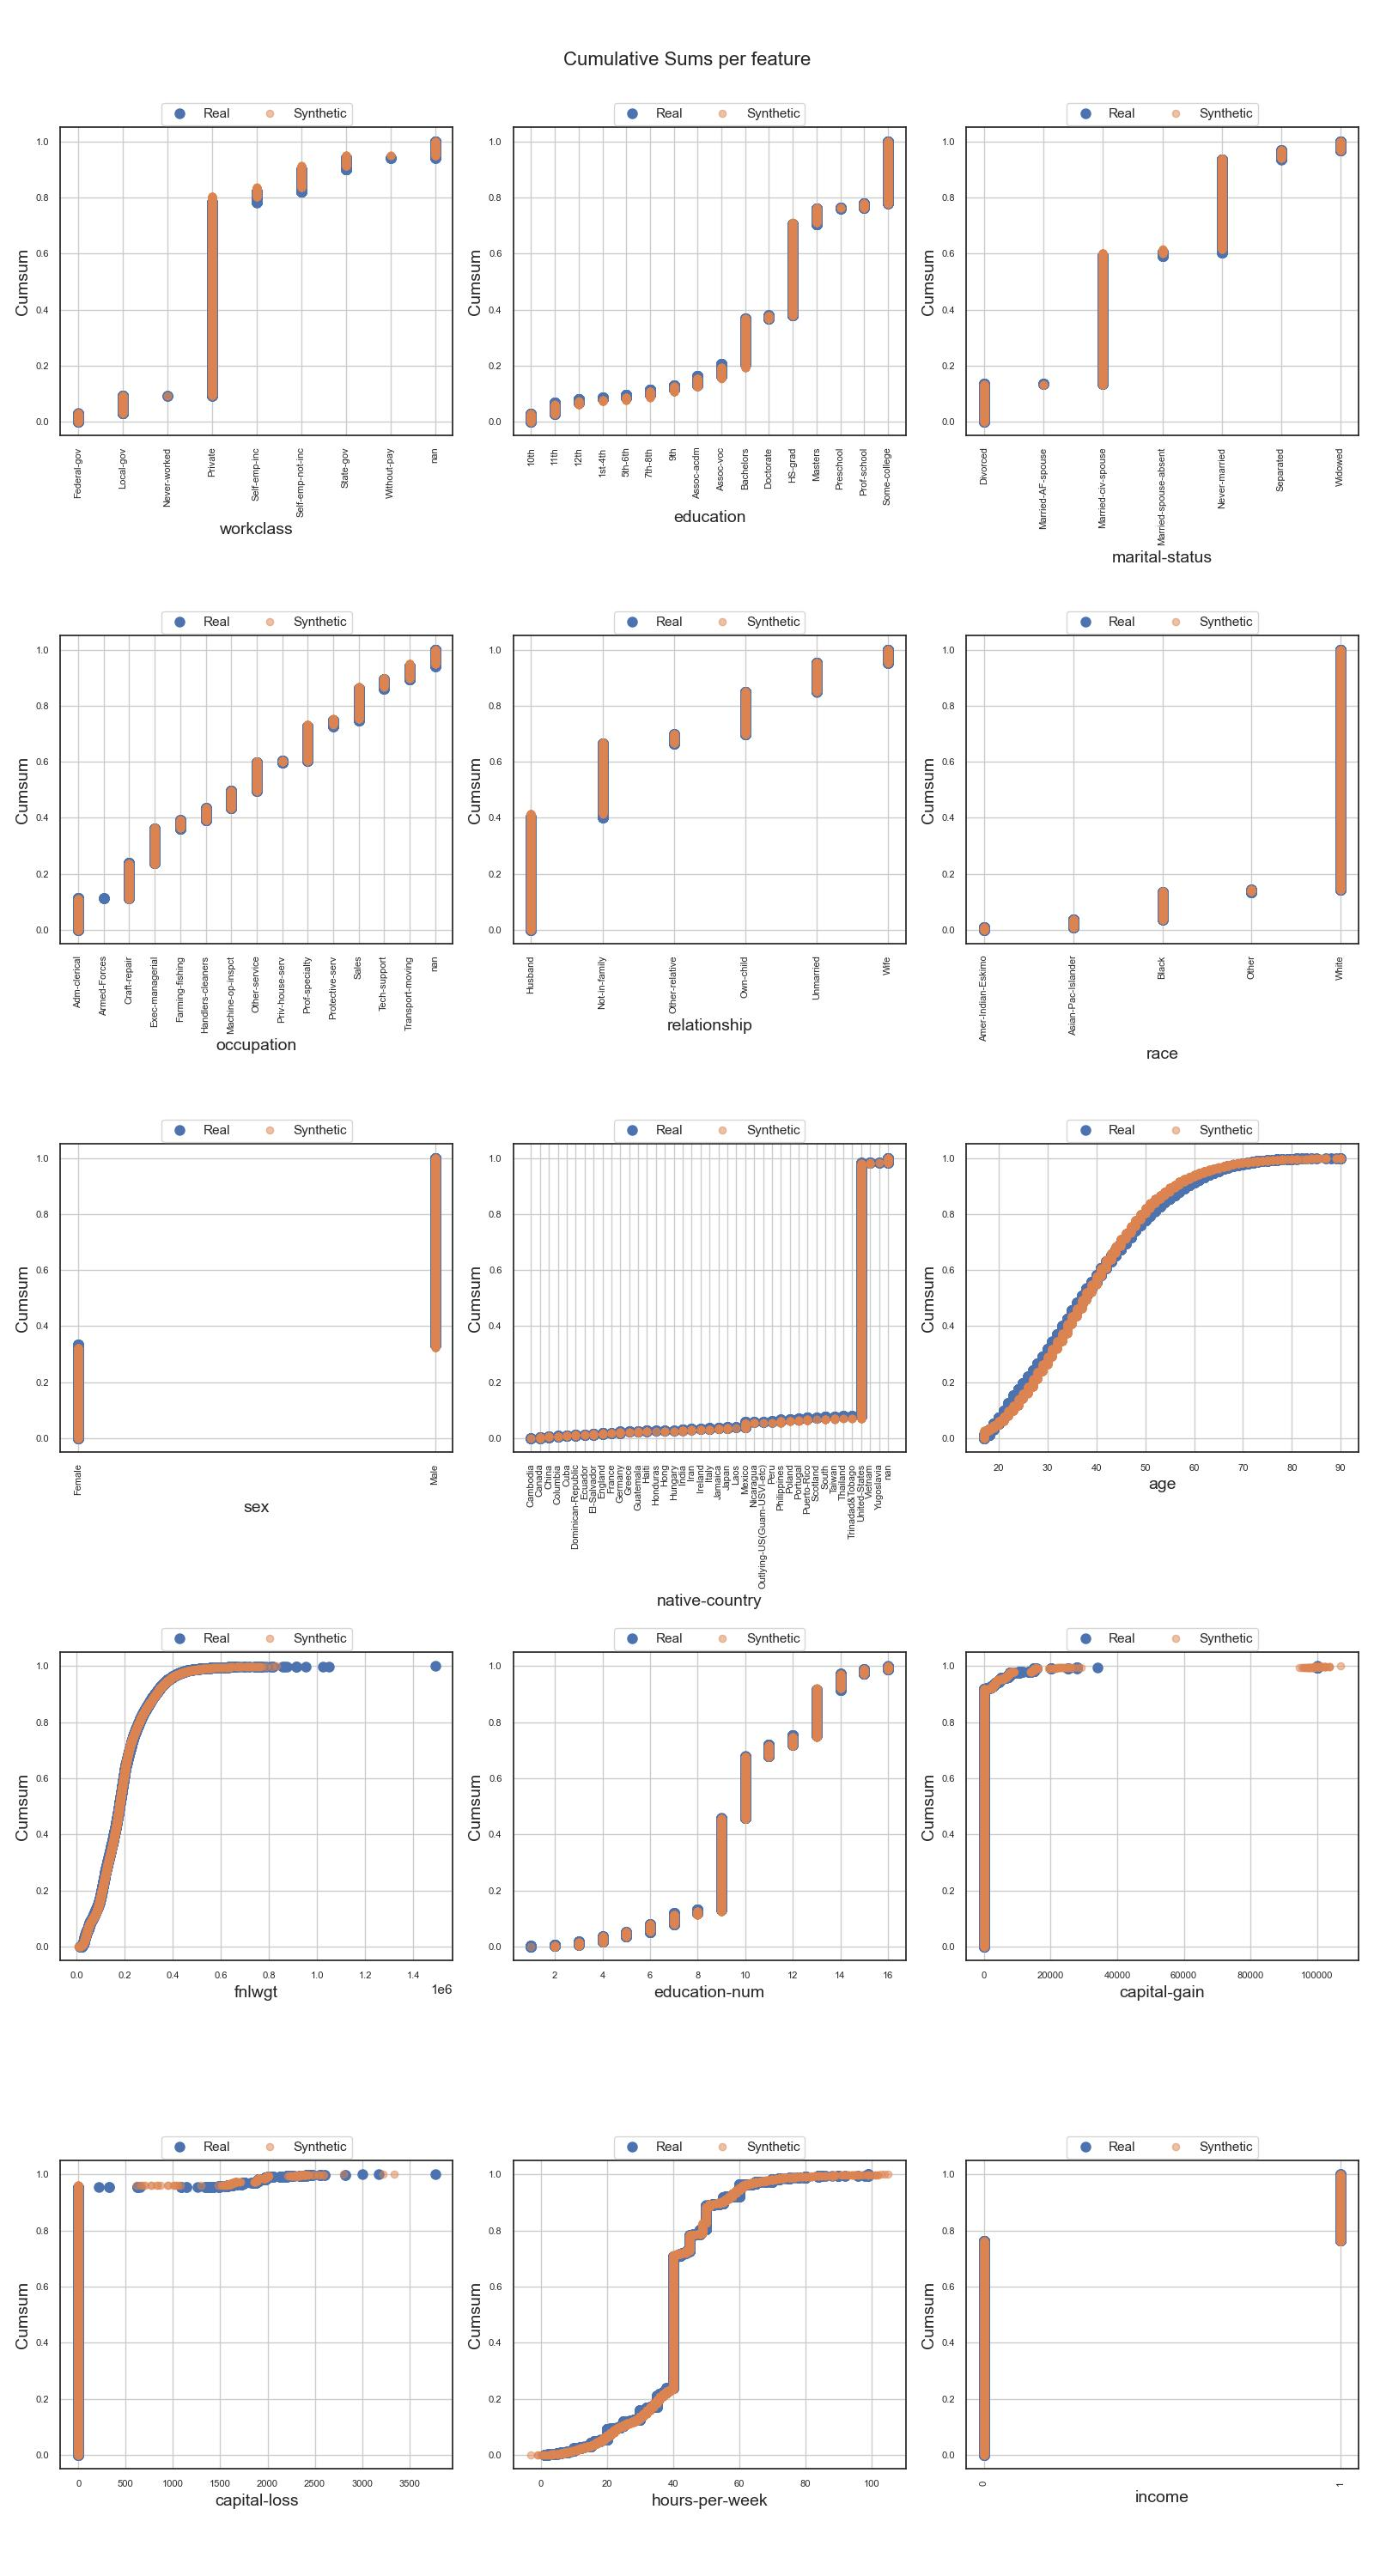
\includegraphics[height=\textheight,width=\linewidth,keepaspectratio]{images/cumsums/tab-ddpm-bgm-simTune-minmax.jpg}
			\caption{TabDDPM-BGM$^{s}_m$}
		\end{subfigure}
		\caption{Cumulative Distribution plots for TabDDPM-BGM variations}
		\label{fig_a:cumsum_4}
	\end{figure}
\end{landscape}
%----------
\newpage
\begin{landscape}
	\begin{figure}[h]
		\centering
		\hfill
		\begin{subfigure}{0.4\linewidth}
			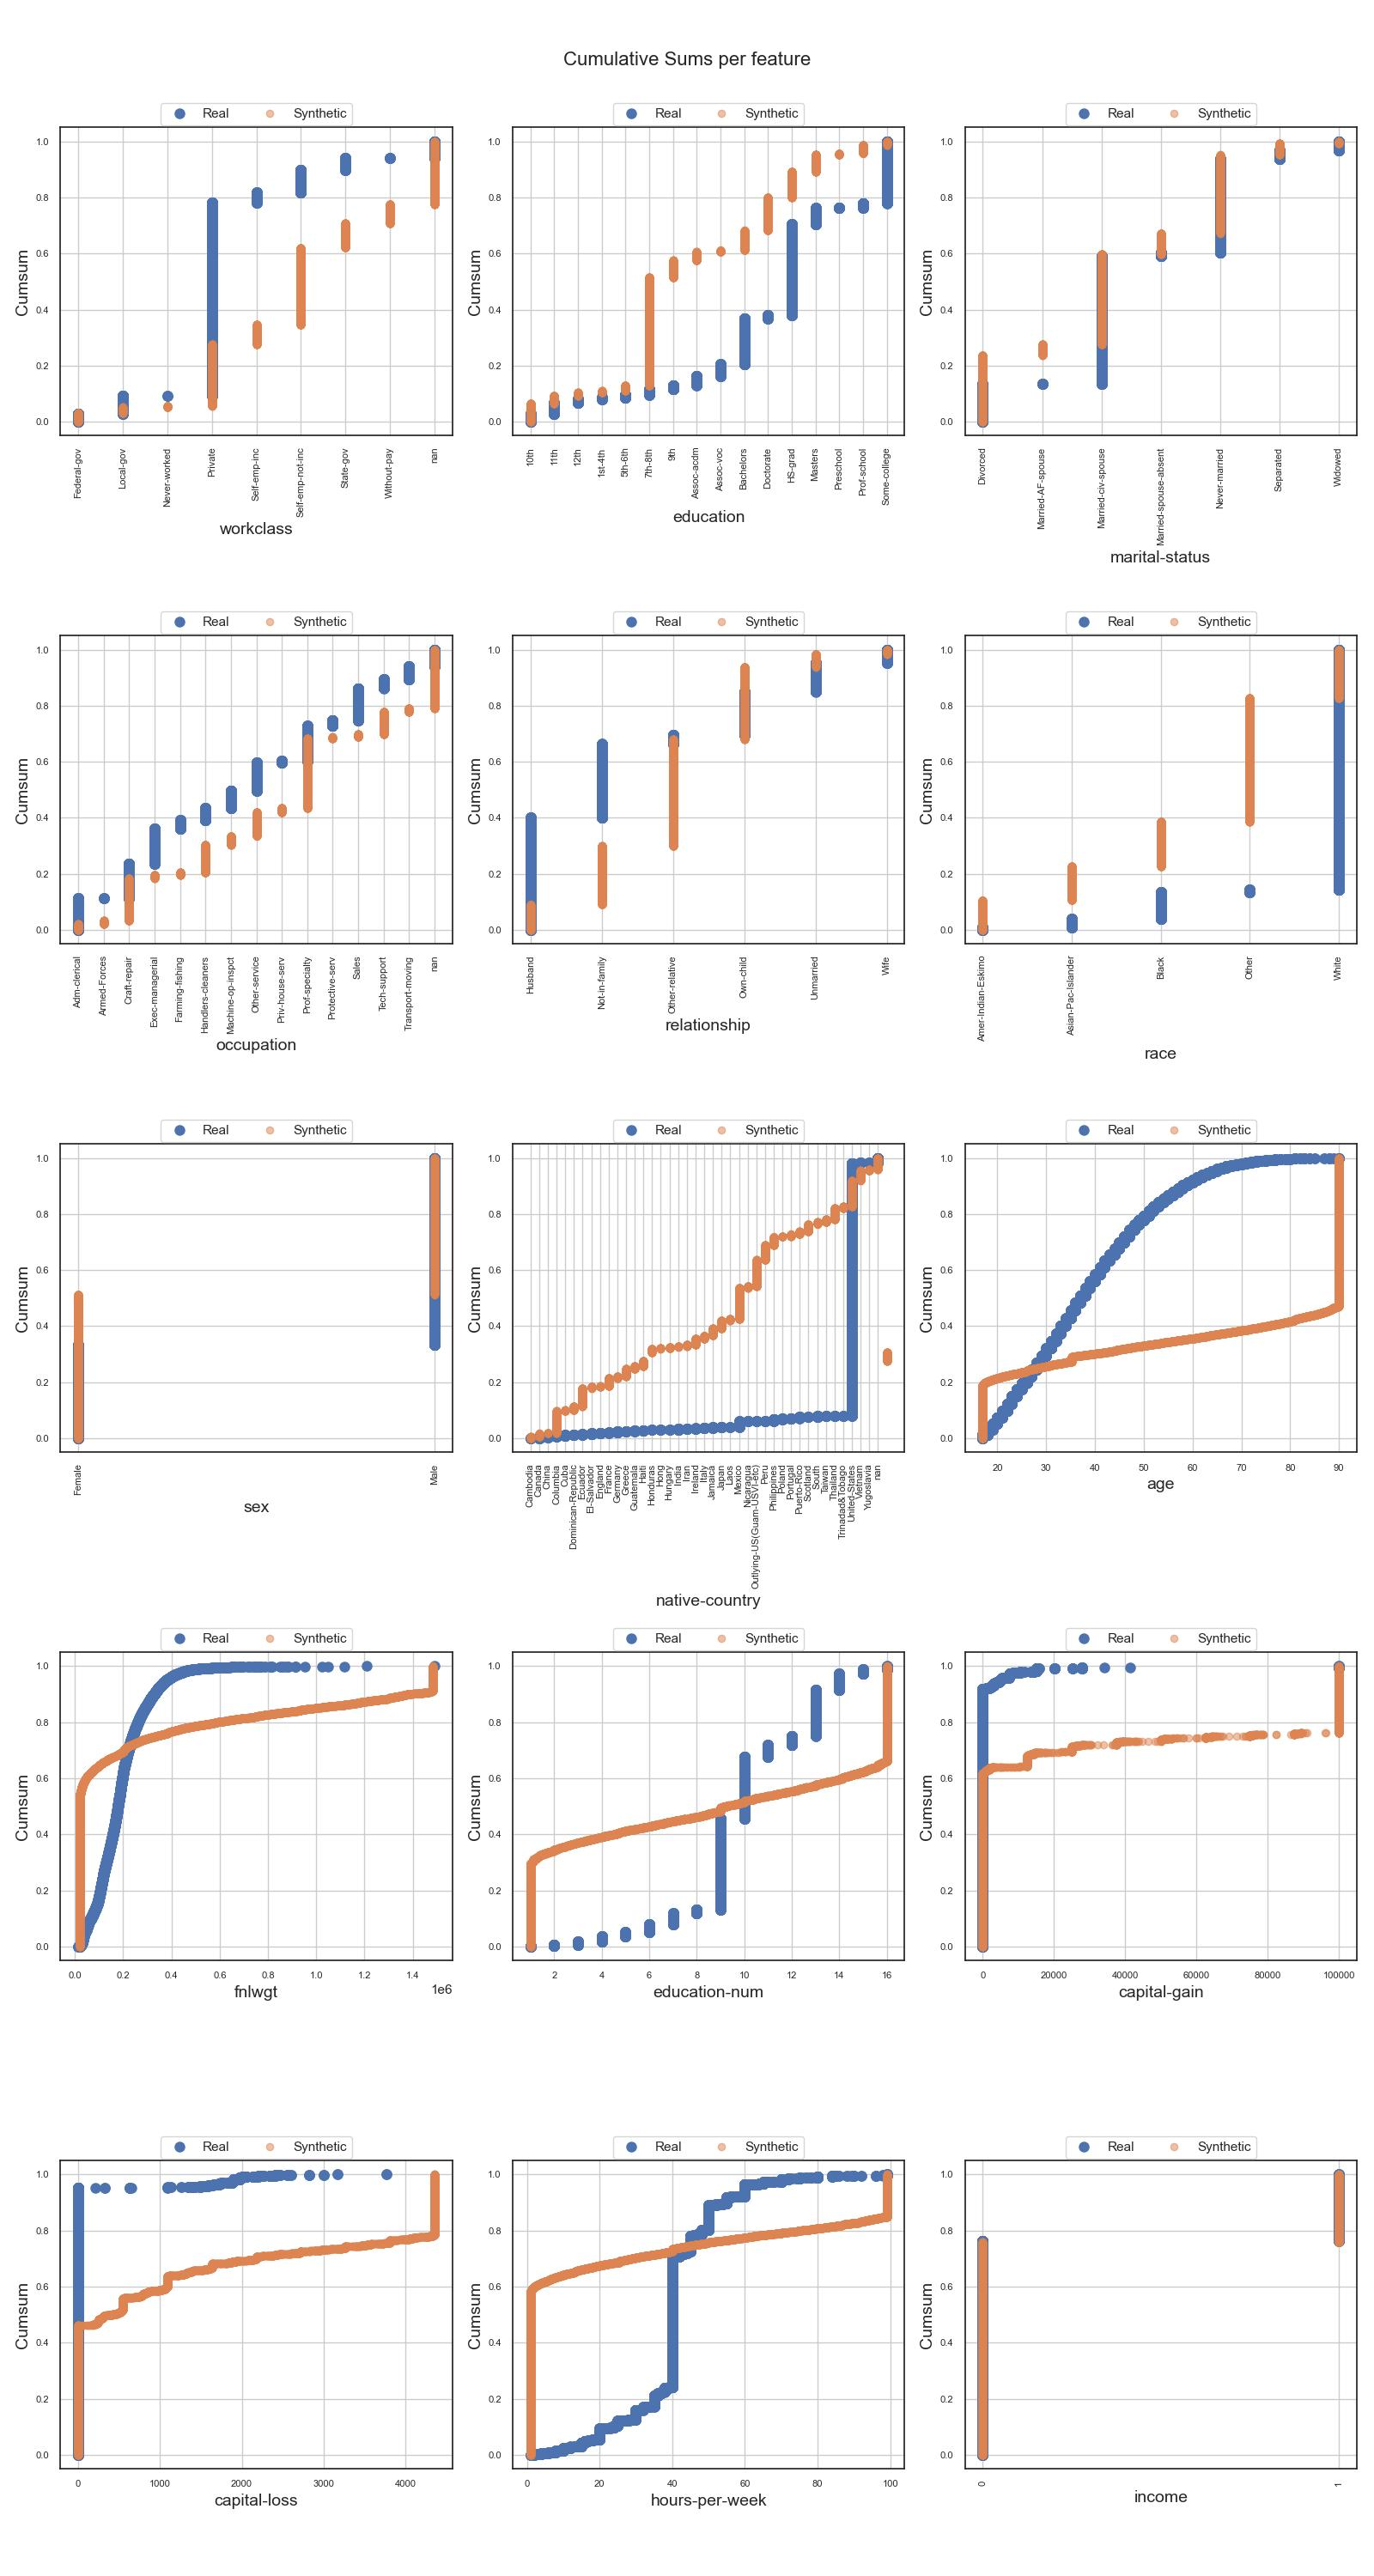
\includegraphics[height=\textheight,width=\linewidth,keepaspectratio]{images/cumsums/tab-ddpm-ft.jpg}
			\caption{TabDDPM-FT$^{ml}_q$}
		\end{subfigure}
		\hfill
		\begin{subfigure}{0.4\linewidth}
			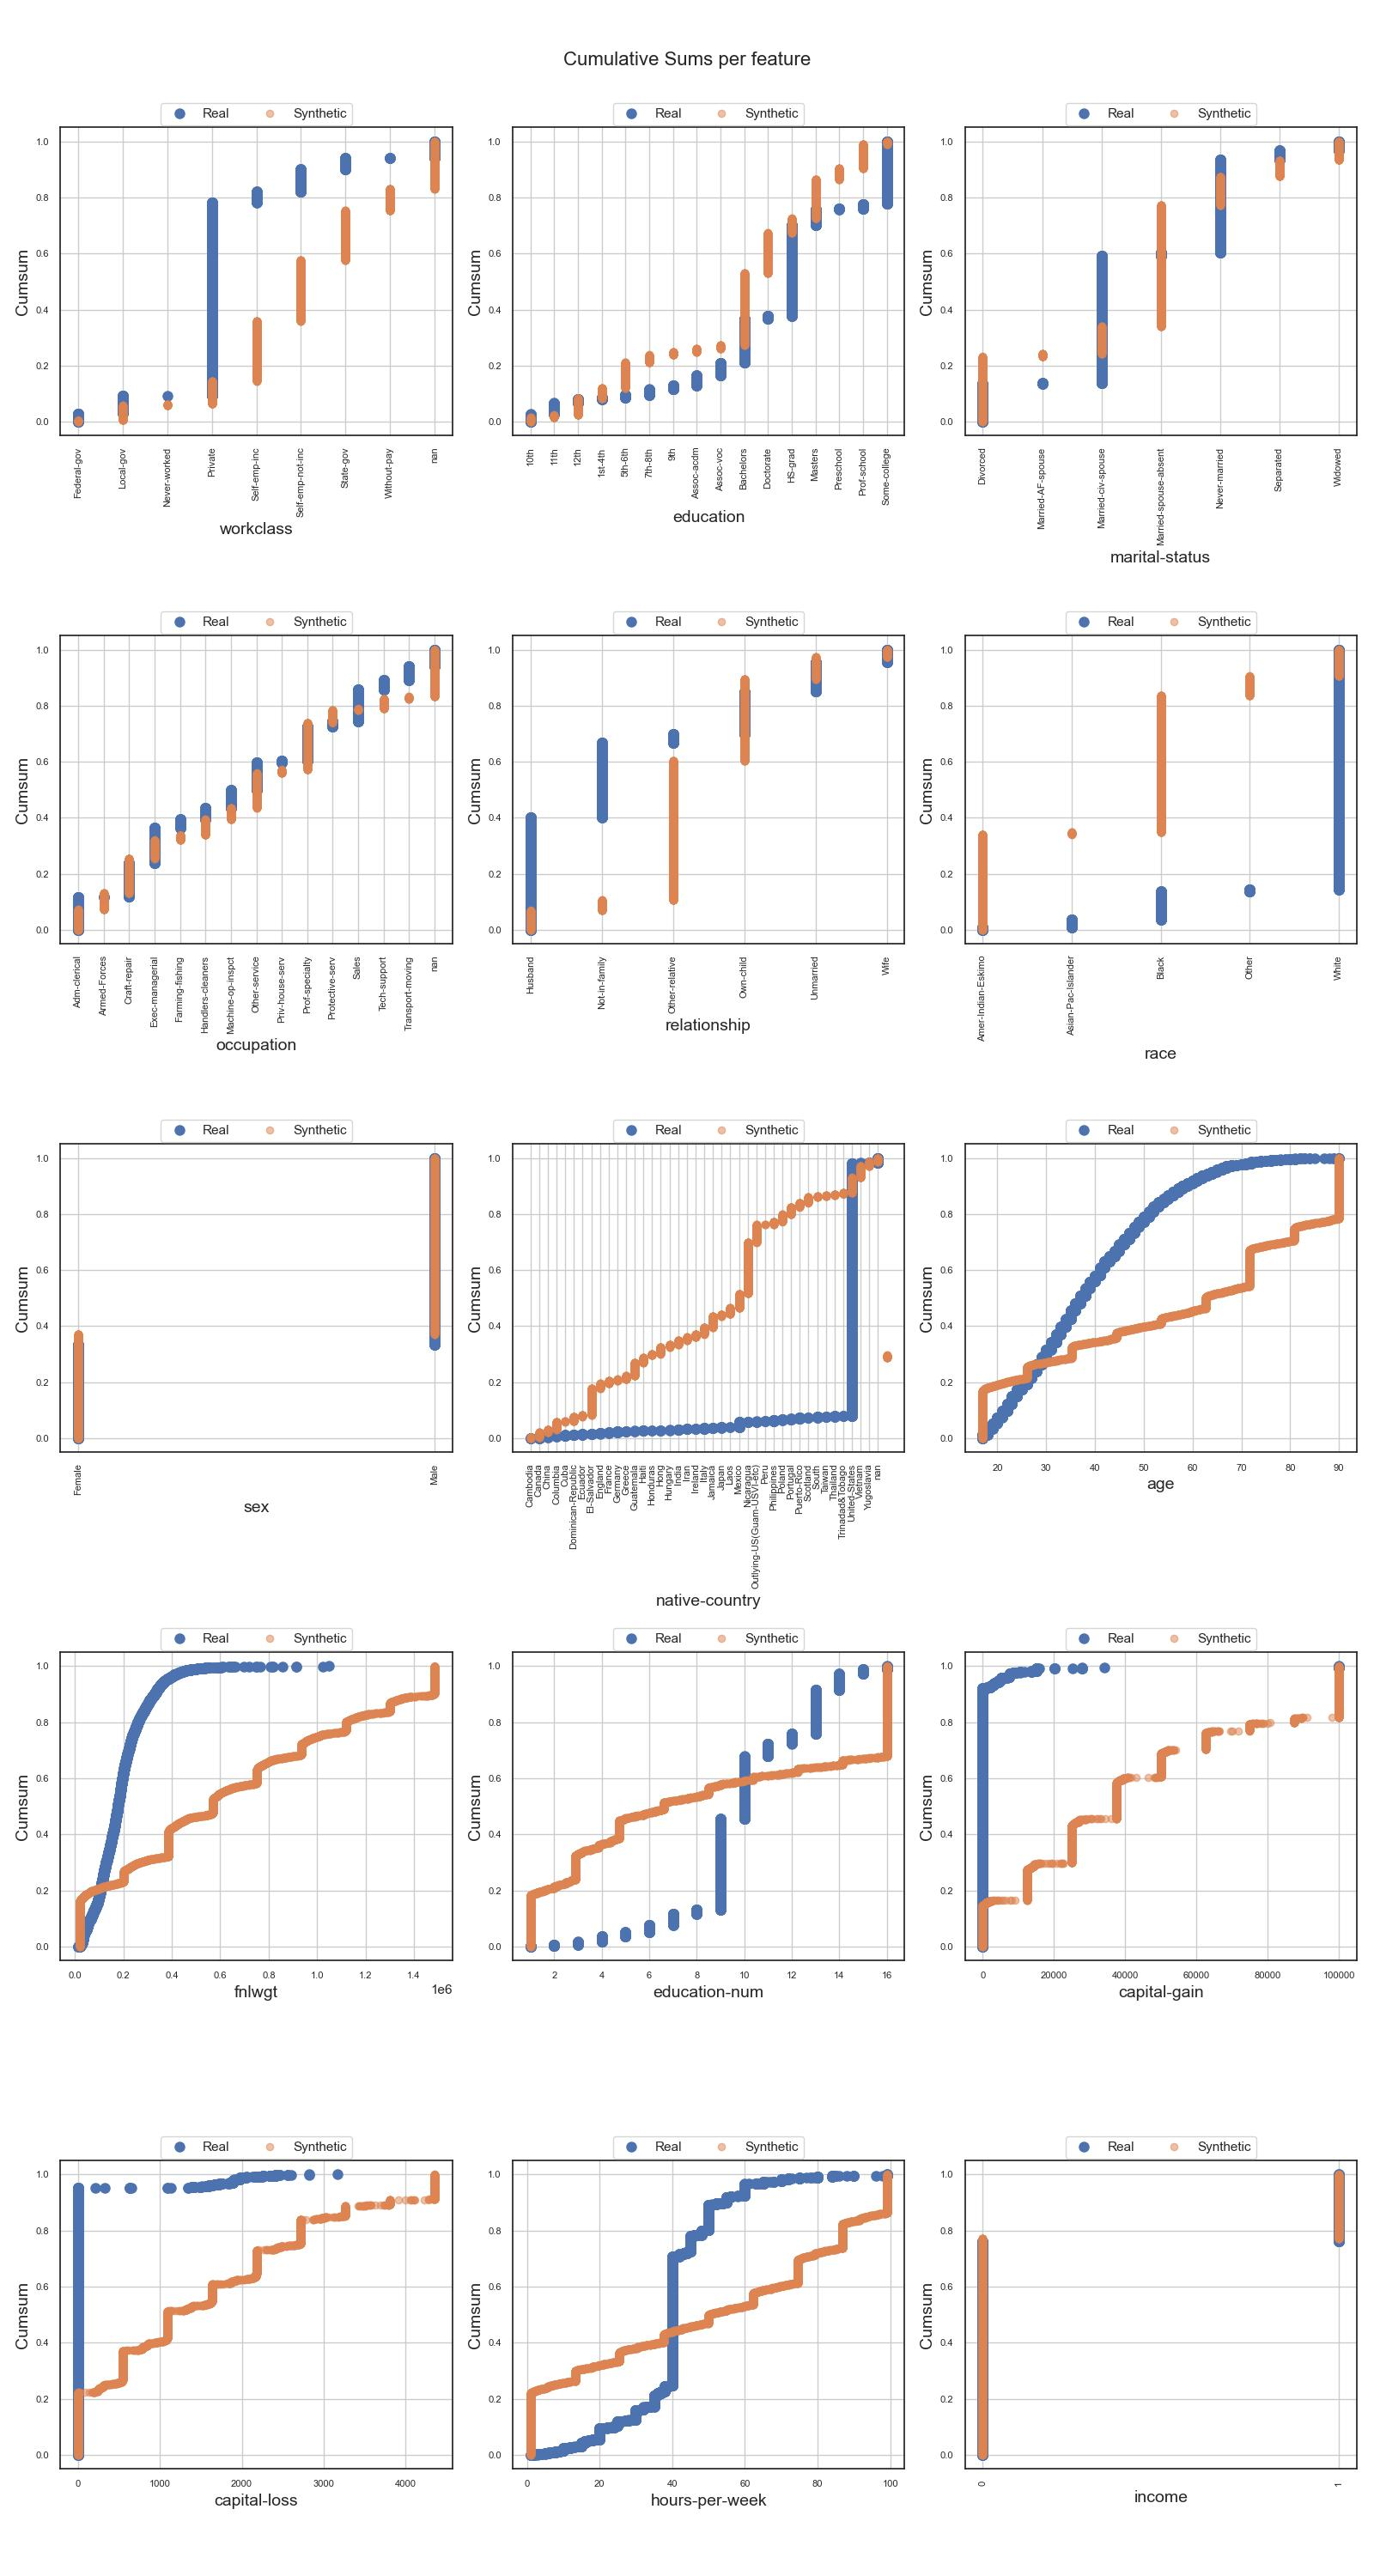
\includegraphics[height=\textheight,width=\linewidth,keepaspectratio]{images/cumsums/tab-ddpm-ft-simTune.jpg}
			\caption{TabDDPM-FT$^{ml}_q$}
		\end{subfigure}
		\caption{Cumulative Distribution plots for TabDDPM-FT variations}
		\label{fig_a:cumsum_5}
	\end{figure}
\end{landscape}







\section*{Extended derivations}
\label{A:derivations}
\subsection*{Diffusion propabilistic models}
Several derivations have been presented in a short format for better readability.
This section will cover left-out derivations.
For a more detailed explanation \cite{weng2021WhatAreDiffusion, outlier2022DiffusionModelsPaper} is recommended.
For further details please refer to \cite{sohl-dickstein2015DeepUnsupervisedLearning, ho2020DenoisingDiffusionProbabilistic}.

Derivation to get from \autoref{eqn:vlb} to \autoref{eqn:vlb2}:

Given:

\begin{equation}
    \label{eqn:kl-divergence_appendix}
    KL(p\parallel q) = \int p(x)\cdot log(\frac{p(x)}{q(x)})dx
\end{equation}

and

\begin{equation}
    \label{eqn:simplify1}
	\begin{align}
    p_\theta(x_{1:T}|x_0) &= \frac{p_\theta(x_0|x_{1:T})p_\theta(x_{1:T})}{p_\theta(x_0)} && \textrm{using bayes rule}\\
	&= \frac{p_\theta(x_0,x_{1:T})}{p_\theta(x_{0})} && \textrm{summarize to joint probability}\\
	&= \frac{p_\theta(x_{0:T})}{p_\theta(x_{0})} && \textrm{summarize to joint probability}\\
\end{align}
\end{equation}

Derivation:

\begin{subequations}
	\label{eqn:vlb2_appendix}
	\begin{align}
		-log(p_\theta(x_0)) &\leq -log(p_\theta(x_0)) + KL(q(x_{1:T}|x_0) \parallel p_\theta(x_{1:T}|x_0)) &&\textrm{}\\
		&= -log(p_\theta(x_0)) + log(\frac{q(x_{1:T})|x_0}{p_\theta(x_{1:T}|x_0)}) && \textrm{using \autoref{eqn:kl-divergence_appendix}}\\
		&=-log(p_\theta(x_0)) + log(\frac{q(x_{1:T})|x_0}{\frac{p_\theta(x_{0:T})}{p_\theta(x_{0})}}) && \textrm{using \autoref{eqn:simplify1}}\\
		&= -log(p_\theta(x_0)) + log(\frac{q(x_{1:T})|x_0}{p_\theta(x_{0:T})})+log(p_\theta(x_{0})) && \textrm{Fraction rule}\\
		&= log(\frac{q(x_{1:T}|x_0)}{p_\theta(x_{0:T})})	&& \textrm{canceling out}\\
		\textrm{Let }L_{VLB} &= \mathbb{E}_{q(x_0:T)}\big[log(\frac{q(x_{1:T}|x_0)}{p_\theta(x_{0:T})}) \big] \geq - \mathbb{E}_{q(x_0)}log(p_\theta(x_0))
	\end{align}
\end{subequations}


Derivation to get from \autoref{eqn:vlb2} to \autoref{eqn:vlb3}:
\begingroup
\small
\begin{subequations}
	\label{eqn:vlb3_appendix}
	\begin{align}
	& L_{VLB}=\mathbb{E}_{q\left(\mathbf{x}_{0: T}\right)}\left[\log \frac{q\left(\mathbf{x}_{1: T} \mid \mathbf{x}_0\right)}{p_\theta\left(\mathbf{x}_{0: T}\right)}\right] \\
	& =\mathbb{E}_q\left[\log \frac{\prod_{t=1}^T q\left(\mathbf{x}_t \mid \mathbf{x}_{t-1}\right)}{p_\theta\left(\mathbf{x}_T\right) \prod_{t=1}^T p_\theta\left(\mathbf{x}_{t-1} \mid \mathbf{x}_t\right)}\right] \\
	& =\mathbb{E}_q\left[-\log p_\theta\left(\mathbf{x}_T\right)+\sum_{t=1}^T \log \frac{q\left(\mathbf{x}_t \mid \mathbf{x}_{t-1}\right)}{p_\theta\left(\mathbf{x}_{t-1} \mid \mathbf{x}_t\right)}\right] \\
	& =\mathbb{E}_q\left[-\log p_\theta\left(\mathbf{x}_T\right)+\sum_{t=2}^T \log \frac{q\left(\mathbf{x}_t \mid \mathbf{x}_{t-1}\right)}{p_\theta\left(\mathbf{x}_{t-1} \mid \mathbf{x}_t\right)}+\log \frac{q\left(\mathbf{x}_1 \mid \mathbf{x}_0\right)}{p_\theta\left(\mathbf{x}_0 \mid \mathbf{x}_1\right)}\right] \\
	& =\mathbb{E}_q\left[-\log p_\theta\left(\mathbf{x}_T\right)+\sum_{t=2}^T \log \left(\frac{q\left(\mathbf{x}_{t-1} \mid \mathbf{x}_t, \mathbf{x}_0\right)}{p_\theta\left(\mathbf{x}_{t-1} \mid \mathbf{x}_t\right)} \cdot \frac{q\left(\mathbf{x}_t \mid \mathbf{x}_0\right)}{q\left(\mathbf{x}_{t-1} \mid \mathbf{x}_0\right)}\right)+\log \frac{q\left(\mathbf{x}_1 \mid \mathbf{x}_0\right)}{p_\theta\left(\mathbf{x}_0 \mid \mathbf{x}_1\right)}\right] \\
	& =\mathbb{E}_q\left[-\log p_\theta\left(\mathbf{x}_T\right)+\sum_{t=2}^T \log \frac{q\left(\mathbf{x}_{t-1} \mid \mathbf{x}_t, \mathbf{x}_0\right)}{p_\theta\left(\mathbf{x}_{t-1} \mid \mathbf{x}_t\right)}+\sum_{t=2}^T \log \frac{q\left(\mathbf{x}_t \mid \mathbf{x}_0\right)}{q\left(\mathbf{x}_{t-1} \mid \mathbf{x}_0\right)}+\log \frac{q\left(\mathbf{x}_1 \mid \mathbf{x}_0\right)}{p_\theta\left(\mathbf{x}_0 \mid \mathbf{x}_1\right)}\right] \\
	& =\mathbb{E}_q\left[-\log p_\theta\left(\mathbf{x}_T\right)+\sum_{t=2}^T \log \frac{q\left(\mathbf{x}_{t-1} \mid \mathbf{x}_t, \mathbf{x}_0\right)}{p_\theta\left(\mathbf{x}_{t-1} \mid \mathbf{x}_t\right)}+\log \frac{q\left(\mathbf{x}_T \mid \mathbf{x}_0\right)}{q\left(\mathbf{x}_1 \mid \mathbf{x}_0\right)}+\log \frac{q\left(\mathbf{x}_1 \mid \mathbf{x}_0\right)}{p_\theta\left(\mathbf{x}_0 \mid \mathbf{x}_1\right)}\right] \\
	& =\mathbb{E}_q\left[\log \frac{q\left(\mathbf{x}_T \mid \mathbf{x}_0\right)}{p_\theta\left(\mathbf{x}_T\right)}+\sum_{t=2}^T \log \frac{q\left(\mathbf{x}_{t-1} \mid \mathbf{x}_t, \mathbf{x}_0\right)}{p_\theta\left(\mathbf{x}_{t-1} \mid \mathbf{x}_t\right)}-\log p_\theta\left(\mathbf{x}_0 \mid \mathbf{x}_1\right)\right] \\
	& =\mathbb{E}_q[\underbrace{D_{\mathrm{KL}}\left(q\left(\mathbf{x}_T \mid \mathbf{x}_0\right) \| p_\theta\left(\mathbf{x}_T\right)\right)}_{L_T}+\sum_{t=2}^T \underbrace{D_{\mathrm{KL}}\left(q\left(\mathbf{x}_{t-1} \mid \mathbf{x}_t, \mathbf{x}_0\right) \| p_\theta\left(\mathbf{x}_{t-1} \mid \mathbf{x}_t\right)\right)}_{L_{t-1}}-\underbrace{\log p_\theta\left(\mathbf{x}_0 \mid \mathbf{x}_1\right)}_{L_0}]
	\end{align}
\end{subequations}
\endgroup
\cleardoublepage

% VERZEICHNISSE (Abbildungen, Tabellen)
% Literatur 
\nocite{wiki:wissarbeit}
\bibliographystyle{alphadin}
\bibliography{Masterarbeit}
\cleardoublepage

% ERKLÄRUNG
\phantomsection
\addcontentsline{toc}{chapter}{Eidesstattliche Versicherung}
% \chapter*{Eidesstattliche Versicherung}
% \thispagestyle{empty}
% \addcontentsline{toc}{chapter}{Eidesstattliche Versicherung}

% Hiermit versichere ich an Eides statt, dass ich die vorliegende Arbeit im Masterstudiengang IT Management und -Consulting selbstständig verfasst und keine anderen als die angegebenen Hilfsmittel - insbesondere keine im Quellenverzeichnis nicht benannten InternetQuellen - benutzt habe. 
% Alle Stellen, die wörtlich oder sinngemäß aus Veröffentlichungen entnommen wurden, sind als solche kenntlich gemacht.
% Ich versichere weiterhin, dass ich die Arbeit vorher nicht in einem anderen Prüfungsverfahren eingereicht habe und die eingereichte schriftliche Fassung der elektronischen Abgabe entspricht.


% \vspace{2cm} 


% \noindent Hamburg, den 21.06.2023 ~~~~~~~~~~~~~~~~~~~~~~~~~Unterschrift: \uline{~~~~~~~~~~~~~~~~~~~~~~~~~~~~~~~~~~~~~~~~~~~~~~~~~~} 

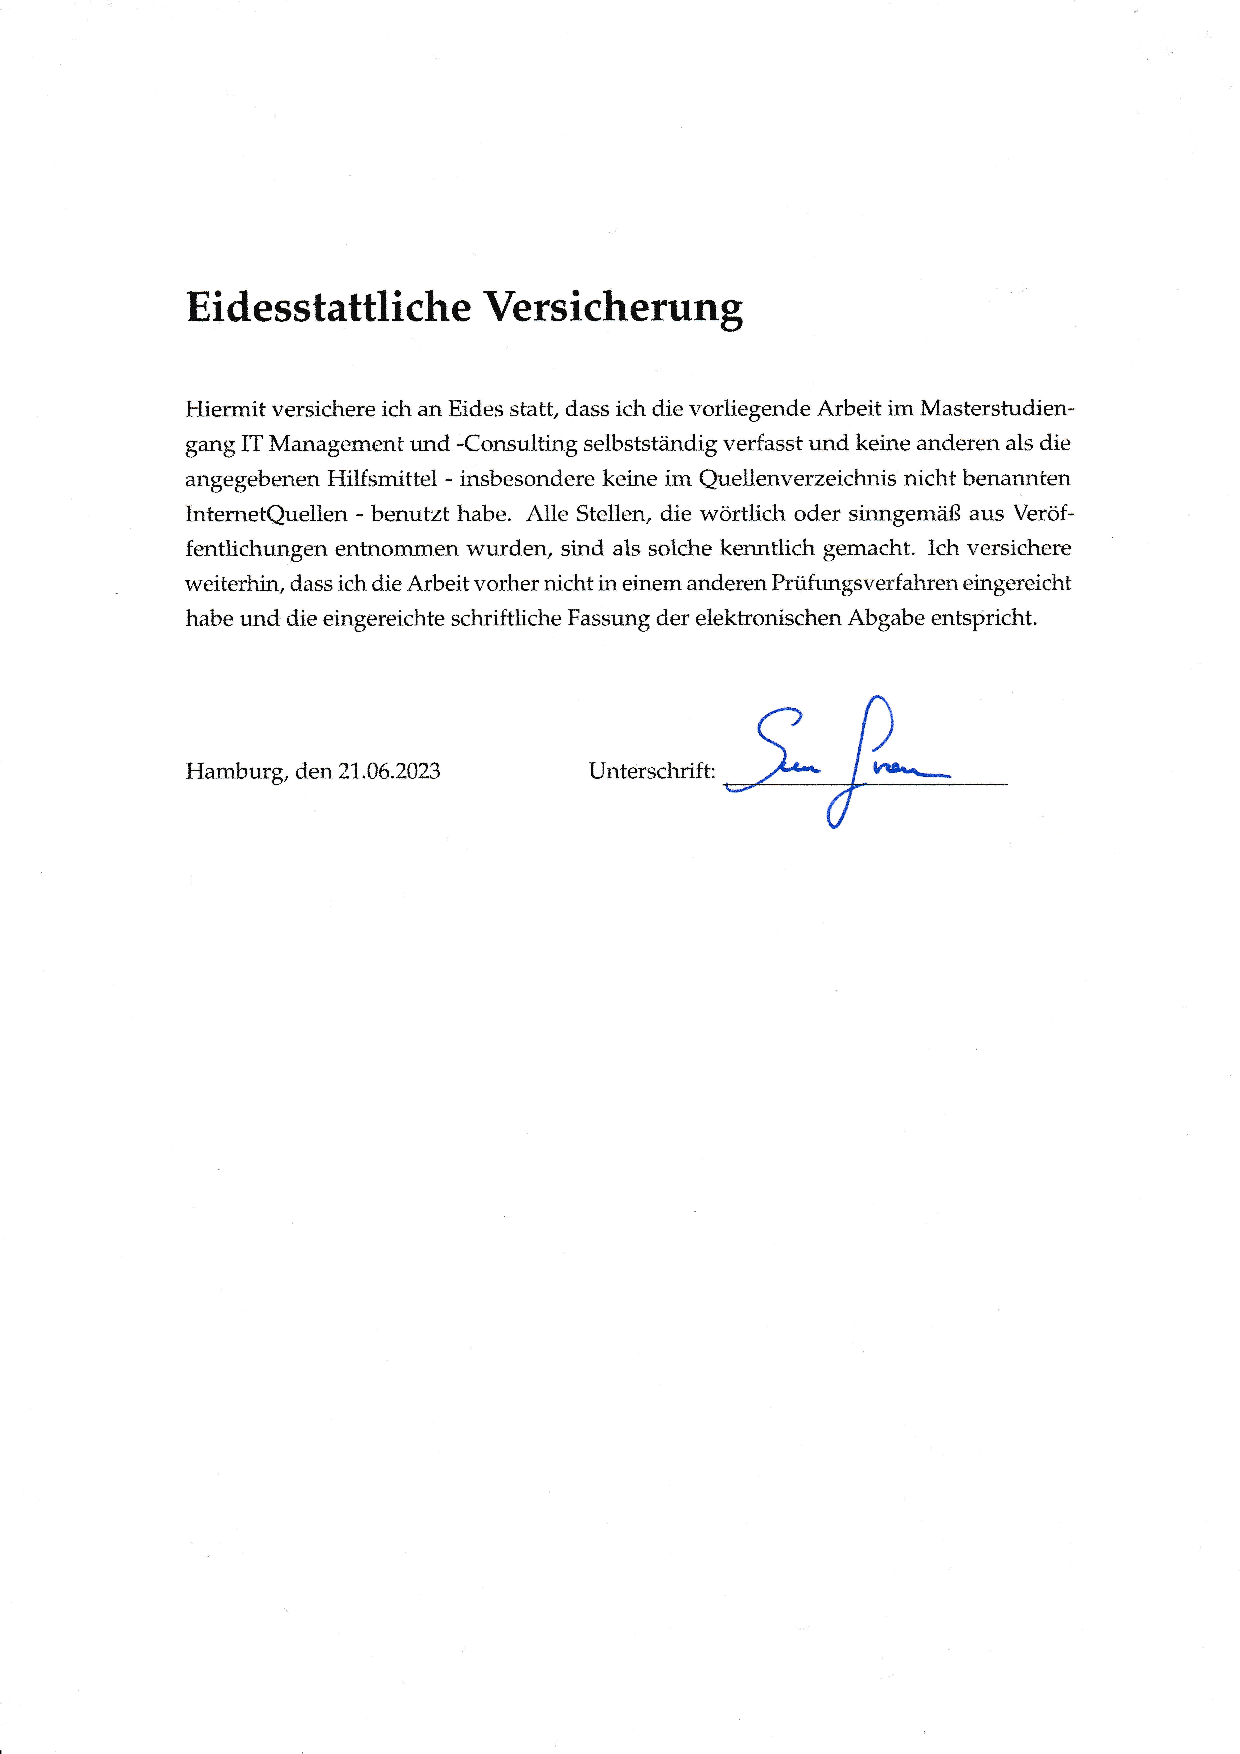
\includepdf[]{Eidesstattliche_Versicherung.pdf}

    
\end{document}